% ============================================================
%  MAIN.TEX
%  Analysis of Market Regimes through Sentiment Extraction
%  from Financial News and Clustering Techniques
%
%  Bachelor's Thesis (TFG) -- Grado en Ingeniería Matemática
%  e Inteligencia Artificial -- ICAI, Universidad Pontificia
%  Comillas
%
%  Author:     Álvaro Fernández Gutiérrez
%  Supervisor: Guillermo Mestre Marcos
% ============================================================
\documentclass[12pt,a4paper,oneside]{report}

% ============================================================
%  PREAMBLE -- Comillas/ICAI style (replicated from Anexo B)
% ============================================================

% --- Page geometry -------------------------------------------------
\usepackage[a4paper,left=3cm,right=2.5cm,top=2.5cm,bottom=2.5cm,headheight=14.5pt]{geometry}

% --- Fonts and encoding ---------------------------------------------
\usepackage[utf8]{inputenc}
\usepackage[T1]{fontenc}
\usepackage{lmodern}
\usepackage{microtype}

% --- Languages (English main document, Spanish "Resumen") ----------
\usepackage[spanish,english]{babel}

% --- Math ------------------------------------------------------------
\usepackage{amsmath}
\usepackage{amssymb}
\usepackage{amsfonts}

% --- Graphics, floats, captions --------------------------------------
\usepackage{graphicx}
\usepackage{float}
\usepackage{caption}
\usepackage{subcaption}
\captionsetup{font=small,labelfont=bf,margin=1cm}

% --- Tables ------------------------------------------------------------
\usepackage{booktabs}
\usepackage{longtable}
\usepackage{array}
\usepackage{multirow}
\usepackage{multicol}
\usepackage{tabularx}
\usepackage{rotating}
\usepackage{pdflscape}

% --- Colour -------------------------------------------------------------
\usepackage[table]{xcolor}

% Comillas/ICAI institutional colour palette (approximate)
\definecolor{comillasblue}{RGB}{0,52,109}
\definecolor{icaigray}{RGB}{89,89,89}
\definecolor{bullgreen}{RGB}{13,122,62}
\definecolor{bearred}{RGB}{192,57,43}
\definecolor{crisisorange}{RGB}{230,126,34}

% --- Headings -------------------------------------------------------------
\usepackage{titlesec}
\titleformat{\chapter}[display]
  {\normalfont\Huge\bfseries\color{comillasblue}}
  {\chaptertitlename\ \thechapter}
  {20pt}{\Huge}
\titlespacing*{\chapter}{0pt}{0pt}{30pt}

% --- Headers and footers (Comillas style) ---------------------------------
\usepackage{fancyhdr}
\pagestyle{fancy}
\fancyhf{}
\renewcommand{\headrulewidth}{0.5pt}
\renewcommand{\footrulewidth}{0pt}
\fancyhead[L]{\small\textsc{Universidad Pontificia Comillas}}
\fancyhead[R]{\small\textsc{ICAI}}
\fancyfoot[C]{\thepage}

\fancypagestyle{plain}{%
  \fancyhf{}
  \fancyfoot[C]{\thepage}
  \renewcommand{\headrulewidth}{0pt}
}

% --- Quotes ---------------------------------------------------------------
\usepackage{csquotes}

% --- Hyperlinks and cross-references (loaded late) -------------------------
\usepackage[hidelinks,colorlinks=false]{hyperref}
\usepackage[capitalize,nameinlink]{cleveref}

% --- Bibliography (biblatex, IEEE numeric style) ----------------------------
\usepackage[backend=biber,style=ieee,sorting=none]{biblatex}
\addbibresource{references.bib}

% --- Acronyms / misc ----------------------------------------------------------
\usepackage{enumitem}
\setlist{noitemsep}

% --- Code listings (for Annex A pipeline description) -------------------------
\usepackage{listings}
\lstset{
  basicstyle=\ttfamily\small,
  breaklines=true,
  frame=single,
  numbers=left,
  numberstyle=\tiny,
  columns=flexible,
  backgroundcolor=\color{gray!8},
}

% --- Helper commands -------------------------------------------------------
\newcommand{\sectionbreak}{\clearpage}

% Title page metadata
\newcommand{\tfgtitle}{Analysis of Market Regimes through Sentiment Extraction from Financial News and Clustering Techniques}
\newcommand{\tfgauthor}{Álvaro Fernández Gutiérrez}
\newcommand{\tfgtutor}{Guillermo Mestre Marcos}
\newcommand{\tfgdegree}{Grado en Ingeniería Matemática e Inteligencia Artificial}
\newcommand{\tfgyear}{2026}


\begin{document}

% ------------------------------------------------------------
% PRELIMINARY PAGES (roman numbering)
% ------------------------------------------------------------
\pagenumbering{roman}

% ============================================================
%  TITLE PAGE -- replicates the Comillas/ICAI cover layout
%  used in Anexo B (UNIVERSIDAD PONTIFICIA COMILLAS / ICAI)
% ============================================================
\begin{titlepage}
\centering

% --- Institutional logo -------------------------------------------------
% TODO: insertar logo oficial ICAI/Comillas (icai_logo.pdf or .png)
\rule{0pt}{2.5cm}
\vspace{0.5cm}

{\scshape\Large Universidad Pontificia Comillas\par}
\vspace{0.2cm}
{\scshape\large Escuela Técnica Superior de Ingeniería (ICAI)\par}
\vspace{0.2cm}
{\scshape\normalsize \tfgdegree\par}

\vspace{1.5cm}
\rule{\linewidth}{0.5pt}
\vspace{0.8cm}

{\Huge\bfseries \tfgtitle \par}

\vspace{0.8cm}
\rule{\linewidth}{0.5pt}
\vspace{2cm}

{\Large Bachelor's Thesis\par}
\vspace{1.5cm}

\begin{flushright}
\begin{minipage}{0.6\textwidth}
\raggedleft
\textbf{Author:}\\
\tfgauthor

\vspace{0.8cm}

\textbf{Supervisor:}\\
\tfgtutor
\end{minipage}
\end{flushright}

\vfill

{\large Madrid, \tfgyear\par}

\end{titlepage}

% ============================================================
%  DECLARATION OF ORIGINALITY (declaración de originalidad)
% ============================================================
\thispagestyle{plain}
\begin{center}
{\bfseries\large DECLARACIÓN DE AUTORÍA Y ORIGINALIDAD}
\end{center}

\vspace{1cm}

\noindent
Declaro, bajo mi responsabilidad, que el Proyecto presentado con el título
\emph{``\tfgtitle''} en la ETS de Ingeniería (ICAI) de la Universidad
Pontificia Comillas en el curso académico \tfgyear\ es de mi autoría,
original e inédito y no ha sido presentado con anterioridad a otros
efectos. El Proyecto no es plagio de otro, ni total ni parcialmente, y la
información que se ha tomado de otros documentos está debidamente
referenciada.

\vspace{3cm}

\begin{flushright}
\begin{minipage}{0.55\textwidth}
\raggedleft
Fdo.: \tfgauthor \\
Fecha: \today

\vspace{2cm}

Autorizada la entrega del proyecto cuando proceda \\

\vspace{1cm}

EL DIRECTOR DEL PROYECTO \\[1.5cm]
Fdo.: \tfgtutor \\
Fecha: \today
\end{minipage}
\end{flushright}

\clearpage

% ============================================================
%  ACKNOWLEDGEMENTS (agradecimientos)
% ============================================================
\thispagestyle{plain}
\begin{center}
{\bfseries\large AGRADECIMIENTOS}
\end{center}

\vspace{1cm}

\noindent
En primer lugar, quiero expresar mi más sincero agradecimiento a mi tutor,
Guillermo Mestre Marcos, por su orientación, disponibilidad y los
comentarios certeros que han guiado este trabajo desde su planteamiento
inicial hasta su forma final. Su apoyo ha sido fundamental para mantener el
rigor metodológico del proyecto en cada una de sus etapas.

\vspace{0.5cm}

\noindent
A la Universidad Pontificia Comillas y a la Escuela Técnica Superior de
Ingeniería (ICAI), por la formación recibida durante estos años de Grado en
Ingeniería Matemática e Inteligencia Artificial, que ha proporcionado las
herramientas matemáticas, estadísticas y computacionales necesarias para
abordar un trabajo de esta naturaleza.

\vspace{0.5cm}

\noindent
A mi familia y amigos, por su paciencia y apoyo incondicional durante todo
el proceso, y por el ánimo constante en los momentos de mayor carga de
trabajo.

\vspace{0.5cm}

\noindent
Por último, a la comunidad de desarrollo de software libre cuyas
herramientas (\textit{Python}, \textit{pandas}, \textit{scikit-learn},
\textit{Hugging Face Transformers}, \textit{hmmlearn}, entre otras) han
hecho posible la implementación completa del pipeline presentado en este
trabajo.

\clearpage


% --- Resumen (Spanish) --------------------------------------
\selectlanguage{spanish}
\chapter*{Resumen del Proyecto}
\addcontentsline{toc}{chapter}{Resumen del Proyecto}
\markboth{Resumen del Proyecto}{Resumen del Proyecto}

Los mercados financieros no se comportan de manera homogénea a lo largo
del tiempo: alternan periodos de crecimiento sostenido, fases de caída
prolongada y episodios de inestabilidad extrema en los que la volatilidad
se dispara y las correlaciones entre activos se rompen. Estos
``regímenes de mercado'' --- habitualmente descritos de forma informal
como mercados \emph{alcistas} (\textit{bull}), \emph{bajistas}
(\textit{bear}) y de \emph{crisis} --- condicionan de manera directa la
gestión del riesgo, la asignación de activos y la toma de decisiones de
inversión. Identificar de forma objetiva y automática en qué régimen se
encuentra el mercado en cada momento es, por tanto, un problema de gran
interés tanto académico como práctico.

La literatura tradicional ha abordado este problema empleando
principalmente variables técnicas y de precio --- rentabilidades,
volatilidad, medias móviles, momentum --- combinadas con métodos
estadísticos como los modelos de Markov de cambio de régimen
(\textit{regime-switching}) o técnicas de aprendizaje no supervisado como
\textit{K-Means}. Sin embargo, estas variables son, por construcción,
\emph{retrospectivas}: reflejan movimientos de precio que ya se han
producido. En paralelo, el auge de los modelos de lenguaje basados en
\textit{Transformers} y, en particular, de modelos especializados en
lenguaje financiero como \textit{FinBERT}, ha abierto la posibilidad de
extraer de manera sistemática el tono emocional --- positivo, negativo o
neutro --- de grandes volúmenes de noticias financieras, proporcionando
una fuente de información \emph{contemporánea} y potencialmente
complementaria a los indicadores técnicos clásicos.

Este Trabajo de Fin de Grado plantea, diseña e implementa un pipeline
completo de extremo a extremo que combina ambas fuentes de información
--- precio/indicadores técnicos y sentimiento extraído de noticias
financieras --- con el objetivo de identificar regímenes de mercado
mediante técnicas de \textit{clustering} no supervisado, y de evaluar de
forma rigurosa si la incorporación del sentimiento mejora la calidad y la
interpretabilidad económica de los regímenes detectados frente a un
enfoque puramente técnico.

\section*{Objetivos}

El objetivo general del proyecto es \textbf{desarrollar y validar una
metodología de detección de regímenes de mercado basada en técnicas de
\textit{clustering}, comparando un modelo que utiliza únicamente
indicadores técnicos del S\&P 500 frente a modelos que incorporan
información de sentimiento sectorial extraída de noticias financieras
mediante FinBERT}. De este objetivo general se derivan los siguientes
objetivos específicos:

\begin{itemize}
  \item Construir un \textit{dataset} unificado que combine indicadores
  técnicos diarios del índice S\&P 500 con un indicador de sentimiento
  agregado por sector GICS, obtenido a partir del conjunto de noticias
  financieras \textit{FNSPID}.
  \item Diseñar y aplicar un procedimiento reproducible de cálculo de
  sentimiento mediante el modelo \textit{FinBERT}, así como un esquema de
  agregación y suavizado temporal de dicho sentimiento a nivel sectorial.
  \item Construir tres modelos de \textit{clustering} (\textit{K-Means})
  alternativos --- técnico, técnico+sentimiento y sentimiento suavizado
  --- y compararlos mediante métricas internas (coeficiente de
  \textit{silhouette}, análisis de componentes principales) e
  \textit{importancia de variables}.
  \item Incorporar un modelo de \textit{Hidden Markov Model} (HMM) como
  método de comparación secundario, evaluando sus diferencias frente a
  \textit{K-Means} en términos de estabilidad temporal y diferenciación
  económica de los regímenes.
  \item Validar económicamente los regímenes obtenidos mediante el
  cálculo de rentabilidad anualizada, volatilidad, \textit{ratio} de
  Sharpe, \textit{drawdown} y otras métricas, desagregadas por sector
  GICS y por régimen.
\end{itemize}

\section*{Metodología}

El pipeline desarrollado, representado de forma esquemática en la
\autoref{fig:resumen-pipeline}, consta de las siguientes etapas
principales:

\begin{enumerate}
  \item \textbf{Adquisición y filtrado de datos}: se parte del
  \textit{dataset} público \textit{FNSPID} (Financial News and Stock
  Price Integration Dataset), que contiene titulares de noticias
  financieras asociados a tickers del mercado estadounidense. Las
  noticias se filtran para conservar únicamente aquellas asociadas a
  empresas que formaban parte del índice S\&P 500 en la fecha de
  publicación correspondiente, y se reasignan al siguiente día de
  mercado abierto para evitar fugas de información (\textit{look-ahead
  bias}).
  \item \textbf{Cálculo de sentimiento con FinBERT}: cada titular se
  procesa con el modelo \textit{ProsusAI/FinBERT}, obteniéndose las
  probabilidades $p_{\text{pos}}$, $p_{\text{neg}}$ y $p_{\text{neu}}$.
  Se define una puntuación de sentimiento continua
  $s = p_{\text{pos}} - p_{\text{neg}} \in [-1,1]$ y una etiqueta
  categórica (positivo/negativo/neutro) obtenida como el argumento
  máximo de las tres probabilidades.
  \item \textbf{Agregación sectorial}: cada ticker se mapea a su sector
  GICS correspondiente (11 sectores), y para cada combinación
  (fecha, sector) se calculan la media y la desviación típica del
  sentimiento de todas las noticias publicadas. Dado el carácter ruidoso
  de la señal diaria, se aplica adicionalmente una media móvil de 21
  sesiones (\textit{MA21}) que reduce sustancialmente el ruido de alta
  frecuencia mientras preserva las tendencias de medio plazo del
  sentimiento sectorial.
  \item \textbf{Indicadores técnicos}: a partir de los precios diarios
  del S\&P 500 se calculan nueve indicadores técnicos --- RSI, ratios
  respecto a medias móviles de 50 y 200 sesiones, \textit{momentum} a 21
  y 126 sesiones, volatilidad realizada a 30 y 252 sesiones, y
  \textit{skewness} de los retornos a 30 y 252 sesiones.
  \item \textbf{Construcción del \textit{dataset} de clustering}: se
  combinan los indicadores técnicos y las variables de sentimiento
  sectorial (\textit{crudas} y suavizadas) en un único \textit{dataset}
  diario, obteniéndose un total de 1132 observaciones en el rango
  comprendido entre mayo de 2009 y febrero de 2024.
  \item \textbf{\textit{Clustering} con K-Means}: se entrenan tres
  modelos --- \textbf{Modelo A} (solo indicadores técnicos), \textbf{Modelo
  B} (indicadores técnicos + sentimiento sectorial crudo) y
  \textbf{Modelo C} (solo sentimiento sectorial suavizado) --- con
  $K=3$, seleccionado mediante el método del codo y el coeficiente de
  \textit{silhouette}. Adicionalmente se entrena un \textbf{modelo HMM}
  (\textit{Gaussian Hidden Markov Model}, covarianza completa, $K=3$
  estados) sobre los mismos conjuntos de variables como método de
  comparación.
  \item \textbf{Etiquetado e interpretación de regímenes}: los
  \textit{clusters} obtenidos se etiquetan como \emph{Bull},
  \emph{Bear} o \emph{Crisis} mediante el análisis de los centroides
  (momentum, volatilidad y RSI medios de cada \textit{cluster}).
  \item \textbf{Validación económica}: para cada combinación de
  sector GICS y régimen se calculan rentabilidad anualizada,
  volatilidad anualizada, \textit{ratio} de Sharpe ($r_f=2\%$),
  \textit{drawdown} máximo, porcentaje de días positivos y los
  retornos diarios extremos (mejor y peor día).
\end{enumerate}

\begin{figure}[H]
  \centering
  % TODO: insertar figura del pipeline completo (diagrama de bloques)
  \fbox{\parbox{0.85\textwidth}{\centering\vspace{3cm}
  Diagrama de bloques del pipeline completo: FNSPID
  $\rightarrow$ filtrado S\&P 500 $\rightarrow$ FinBERT $\rightarrow$
  agregación sectorial GICS (media/std + MA21) $\rightarrow$ indicadores
  técnicos S\&P 500 $\rightarrow$ \textit{dataset} de clustering
  $\rightarrow$ K-Means (Modelos A/B/C) y HMM $\rightarrow$ validación
  económica por sector y régimen.\vspace{3cm}}}
  \caption{Esquema general del pipeline desarrollado en este proyecto.}
  \label{fig:resumen-pipeline}
\end{figure}

\section*{Resultados principales}

El análisis del coeficiente de \textit{silhouette} en un espacio común de
componentes principales (reteniendo el 80\% de la varianza explicada)
muestra que el \textbf{Modelo A (técnico)} obtiene la mejor cohesión
interna (\textit{silhouette} $\approx 0.193$), seguido del \textbf{Modelo
B (técnico + sentimiento)} ($\approx 0.178$) y, por último, del
\textbf{Modelo C (solo sentimiento suavizado)} ($\approx 0.162$). Esto
indica que las variables técnicas siguen siendo las que mejor separan
estructuralmente los datos, y que el sentimiento por sí solo no es
suficiente para definir \textit{clusters} bien diferenciados.

Sin embargo, la \textbf{validación económica} revela un panorama más
matizado. El Modelo B, que incorpora sentimiento sectorial junto con los
indicadores técnicos, produce regímenes con una diferenciación económica
\emph{más marcada} que el Modelo A: el régimen \emph{Bear} del Modelo B
presenta \textit{ratios} de Sharpe negativos en prácticamente todos los
sectores (p.\ ej., $-0.36$ en \textit{Financial Services} o $-0.26$ en
\textit{Energy}), mientras que el régimen \emph{Crisis} concentra, de
forma contraintuitiva, las rentabilidades anualizadas más elevadas (hasta
$+91.9\%$ en \textit{Real Estate}), reflejando episodios de alta
volatilidad con fuertes recuperaciones (\textit{rebounds}). El sector
\textit{Energy} en régimen \emph{Bear} presenta el \textit{drawdown}
máximo más severo de todo el análisis ($-74.9\%$), así como el mejor y el
peor día individual de toda la muestra ($+16.9\%$ y $-24.7\%$,
respectivamente), lo que evidencia la naturaleza extremadamente volátil
de dicho régimen.

El \textbf{Modelo C}, basado exclusivamente en sentimiento suavizado,
produce centroides prácticamente indistinguibles en las variables
técnicas (p.\ ej., el ratio respecto a la media móvil de 50 sesiones varía
entre 1.0086 y 1.0134 entre regímenes), lo que constituye un
\emph{resultado negativo relevante}: el sentimiento agregado por sí solo,
sin información de precio, no logra capturar la dinámica de los regímenes
de mercado con la misma nitidez que los indicadores técnicos.

La comparación con el modelo \textbf{HMM} muestra que, si bien ambos
métodos identifican regímenes cualitativamente similares, \textit{K-Means}
produce una diferenciación económica \emph{mucho más pronunciada} entre
regímenes (\textit{ratios} de Sharpe que oscilan aproximadamente entre
$-3.1$ y $+3.8$), mientras que el HMM genera estados con \textit{ratios}
de Sharpe mucho más moderados (entre $-0.6$ y $+1.5$ aproximadamente),
consistente con su naturaleza de modelo generativo con transiciones
suaves entre estados.

\section*{Conclusiones}

Los resultados obtenidos confirman que los indicadores técnicos
constituyen la base más sólida para la detección de regímenes de mercado
mediante \textit{clustering}, pero que la incorporación de sentimiento
sectorial extraído mediante FinBERT \textbf{aporta valor incremental en
términos de diferenciación económica} de los regímenes resultantes, en
particular para distinguir episodios de \emph{Bear market} sostenido
frente a episodios de \emph{Crisis} de alta volatilidad con fuertes
oscilaciones. Estos hallazgos abren la puerta a líneas de trabajo futuras
orientadas a la combinación dinámica de ambas fuentes de información, a
la extensión del análisis a otros índices y mercados, y a la exploración
de arquitecturas de \textit{deep learning} secuenciales para la detección
de regímenes.

\vspace{1cm}
\noindent\textbf{Palabras clave:} regímenes de mercado, \textit{clustering},
K-Means, \textit{Hidden Markov Model}, análisis de sentimiento, FinBERT,
noticias financieras, FNSPID, S\&P 500, validación económica.

\clearpage

\selectlanguage{english}

% --- Abstract (English) ---------------------------------------
\chapter*{Abstract}
\addcontentsline{toc}{chapter}{Abstract}
\markboth{Abstract}{Abstract}

Financial markets do not behave homogeneously over time. Instead, they
alternate between periods of sustained growth, prolonged downturns, and
episodes of extreme instability in which volatility spikes and
cross-asset correlations break down. These ``market regimes'' ---
informally described as \emph{bull}, \emph{bear} and \emph{crisis}
markets --- have a direct impact on risk management, asset allocation
and investment decision-making. Identifying, in an objective and
automated manner, which regime the market is currently in is therefore a
problem of substantial academic and practical interest.

Traditional approaches to this problem rely mainly on price-based and
technical variables --- returns, volatility, moving averages, momentum
--- combined with statistical methods such as regime-switching models or
unsupervised learning techniques like \textit{K-Means}. However, these
variables are, by construction, \emph{backward-looking}: they reflect
price movements that have already occurred. At the same time, the rise of
\textit{Transformer}-based language models, and in particular of
finance-specific models such as \textit{FinBERT}, has made it possible to
systematically extract the emotional tone --- positive, negative or
neutral --- of large volumes of financial news, providing a
\emph{contemporaneous} source of information that is potentially
complementary to classical technical indicators.

This Bachelor's Thesis designs and implements a complete end-to-end
pipeline that combines both sources of information --- price/technical
indicators and sentiment extracted from financial news --- with the goal
of identifying market regimes through unsupervised clustering techniques,
and of rigorously assessing whether incorporating sentiment improves the
quality and economic interpretability of the resulting regimes compared
to a purely technical approach.

\section*{Objectives}

The overall objective of this project is to \textbf{develop and validate
a clustering-based market regime detection methodology, comparing a model
that relies exclusively on S\&P 500 technical indicators against models
that additionally incorporate sector-level sentiment extracted from
financial news using FinBERT}. This overall objective is broken down into
the following specific objectives:

\begin{itemize}
  \item Build a unified dataset combining daily technical indicators for
  the S\&P 500 index with a sector-level (GICS) sentiment indicator
  derived from the \textit{FNSPID} financial news corpus.
  \item Design and implement a reproducible sentiment-scoring procedure
  based on the \textit{FinBERT} model, together with a sector-level
  aggregation and temporal smoothing scheme.
  \item Build three alternative \textit{K-Means} clustering models ---
  technical-only, technical+sentiment and smoothed-sentiment-only --- and
  compare them using internal validation metrics (silhouette coefficient,
  principal component analysis) and feature-importance analysis.
  \item Incorporate a \textit{Hidden Markov Model} (HMM) as a secondary
  comparison method, evaluating its differences with respect to
  \textit{K-Means} in terms of temporal stability and economic
  differentiation of the regimes.
  \item Economically validate the obtained regimes by computing
  annualized return, volatility, Sharpe ratio, drawdown and other
  metrics, broken down by GICS sector and by regime.
\end{itemize}

\section*{Methodology}

The developed pipeline, schematically represented in
\autoref{fig:abstract-pipeline}, consists of the following main stages:

\begin{enumerate}
  \item \textbf{Data acquisition and filtering}: the starting point is
  the public \textit{FNSPID} (Financial News and Stock Price Integration
  Dataset) corpus, which contains financial news headlines associated
  with US-market tickers. News items are filtered to retain only those
  associated with companies that were constituents of the S\&P 500 at the
  time of publication, and are reassigned to the next open market day to
  avoid look-ahead bias.
  \item \textbf{Sentiment scoring with FinBERT}: each headline is
  processed with the \textit{ProsusAI/FinBERT} model, yielding
  probabilities $p_{\text{pos}}$, $p_{\text{neg}}$ and $p_{\text{neu}}$. A
  continuous sentiment score $s = p_{\text{pos}} - p_{\text{neg}} \in
  [-1,1]$ is defined, together with a categorical label
  (positive/negative/neutral) obtained as the argmax of the three
  probabilities.
  \item \textbf{Sector-level aggregation}: each ticker is mapped to its
  corresponding GICS sector (11 sectors), and for each (date, sector)
  combination the mean and standard deviation of sentiment across all
  published news items are computed. Given the noisy nature of the daily
  signal, a 21-session moving average (\textit{MA21}) is additionally
  applied, which substantially reduces high-frequency noise while
  preserving medium-term trends in sector sentiment.
  \item \textbf{Technical indicators}: nine technical indicators are
  computed from daily S\&P 500 prices --- RSI, 50- and 200-session moving
  average ratios, 21- and 126-session momentum, 30- and 252-session
  realized volatility, and 30- and 252-session return skewness.
  \item \textbf{Clustering dataset construction}: technical indicators and
  sector-level sentiment variables (raw and smoothed) are merged into a
  single daily dataset, resulting in 1,132 observations spanning May 2009
  to February 2024.
  \item \textbf{K-Means clustering}: three models are trained ---
  \textbf{Model A} (technical indicators only), \textbf{Model B}
  (technical indicators + raw sector sentiment) and \textbf{Model C}
  (smoothed sector sentiment only) --- with $K=3$, selected via the elbow
  method and the silhouette coefficient. In addition, a \textbf{Gaussian
  HMM} (full covariance, $K=3$ states) is trained on the same feature sets
  as a comparison method.
  \item \textbf{Regime labeling and interpretation}: the resulting
  clusters are labeled as \emph{Bull}, \emph{Bear} or \emph{Crisis} based
  on centroid analysis (mean momentum, volatility and RSI of each
  cluster).
  \item \textbf{Economic validation}: for each combination of GICS sector
  and regime, annualized return, annualized volatility, Sharpe ratio
  ($r_f=2\%$), maximum drawdown, percentage of positive days and extreme
  daily returns (best and worst day) are computed.
\end{enumerate}

\begin{figure}[H]
  \centering
  % TODO: insert full pipeline diagram (block diagram)
  \fbox{\parbox{0.85\textwidth}{\centering\vspace{3cm}
  Block diagram of the complete pipeline: FNSPID
  $\rightarrow$ S\&P 500 filtering $\rightarrow$ FinBERT $\rightarrow$
  GICS sector aggregation (mean/std + MA21) $\rightarrow$ S\&P 500
  technical indicators $\rightarrow$ clustering dataset $\rightarrow$
  K-Means (Models A/B/C) and HMM $\rightarrow$ economic validation by
  sector and regime.\vspace{3cm}}}
  \caption{General overview of the pipeline developed in this project.}
  \label{fig:abstract-pipeline}
\end{figure}

\section*{Main results}

Silhouette analysis in a common principal-component space (retaining 80\%
of explained variance) shows that \textbf{Model A (technical)} achieves
the best internal cohesion (silhouette $\approx 0.193$), followed by
\textbf{Model B (technical + sentiment)} ($\approx 0.178$) and
\textbf{Model C (smoothed sentiment only)} ($\approx 0.162$). This
indicates that technical variables remain the strongest structural
discriminators of the data, and that sentiment alone is not sufficient to
define well-separated clusters.

However, \textbf{economic validation} reveals a more nuanced picture.
Model B, which incorporates sector sentiment alongside technical
indicators, produces regimes with \emph{sharper} economic differentiation
than Model A: the \emph{Bear} regime of Model B exhibits negative Sharpe
ratios across virtually all sectors (e.g., $-0.36$ for \textit{Financial
Services} and $-0.26$ for \textit{Energy}), while the \emph{Crisis} regime
counter-intuitively concentrates the highest annualized returns (up to
$+91.9\%$ for \textit{Real Estate}), reflecting high-volatility episodes
with strong rebounds. The \textit{Energy} sector in the \emph{Bear} regime
exhibits the most severe maximum drawdown of the entire analysis
($-74.9\%$), as well as the best and worst single-day returns of the whole
sample ($+16.9\%$ and $-24.7\%$, respectively), highlighting the extremely
volatile nature of this regime.

\textbf{Model C}, based exclusively on smoothed sentiment, produces
centroids that are nearly indistinguishable in technical variables (e.g.,
the 50-session moving-average ratio ranges from 1.0086 to 1.0134 across
regimes), constituting a \emph{meaningful negative result}: aggregated
sentiment alone, without price information, fails to capture market
regime dynamics with the same sharpness as technical indicators.

The comparison with the \textbf{HMM} model shows that, while both methods
identify qualitatively similar regimes, \textit{K-Means} produces a
\emph{much sharper} economic differentiation between regimes (Sharpe
ratios ranging approximately from $-3.1$ to $+3.8$), whereas the HMM
generates states with much milder Sharpe ratios (roughly between $-0.6$
and $+1.5$), consistent with its nature as a generative model with smooth
transitions between states.

\section*{Conclusions}

The results obtained confirm that technical indicators provide the
strongest foundation for clustering-based market regime detection, but
that incorporating sector-level sentiment extracted via FinBERT
\textbf{adds incremental value in terms of the economic differentiation}
of the resulting regimes, particularly for distinguishing sustained
\emph{bear-market} episodes from high-volatility \emph{crisis} episodes
with sharp rebounds. These findings open avenues for future work focused
on the dynamic combination of both information sources, the extension of
the analysis to other indices and markets, and the exploration of
sequential deep-learning architectures for regime detection.

\vspace{1cm}
\noindent\textbf{Keywords:} market regimes, clustering, K-Means, Hidden
Markov Model, sentiment analysis, FinBERT, financial news, FNSPID, S\&P
500, economic validation.

\clearpage


% --- Tables of contents, figures, tables ------------------------
\tableofcontents
\clearpage
\listoffigures
\clearpage
\listoftables
\clearpage

% ------------------------------------------------------------
% MAIN MATTER (arabic numbering)
% ------------------------------------------------------------
\pagenumbering{arabic}
\setcounter{page}{1}

\chapter{Introduction}
\label{ch:introduction}

\section{Motivation and Context}
\label{sec:motivation}

Financial markets are dynamic systems whose statistical properties change
substantially over time. Returns that are approximately stationary during
extended periods of economic expansion can suddenly give way to regimes
characterized by negative drift, elevated volatility, and strong
cross-sectional co-movement across assets and sectors. The global
financial crisis of 2008 and the COVID-19 market crash of March 2020 are
two of the most salient examples of this phenomenon in recent history. In
both episodes, equity indices such as the S\&P 500 experienced drawdowns
exceeding 30\% within a few weeks, volatility indices reached historical
highs, and the correlation structure between sectors that are normally
weakly related --- for instance, \textit{Energy} and \textit{Information
Technology} --- increased sharply, a hallmark of what the literature
broadly refers to as a \emph{crisis regime} \cite{ang2002regime}.

The notion that financial markets alternate between a small number of
distinct \emph{regimes} --- commonly described informally as
\emph{bull}, \emph{bear} and \emph{crisis} markets --- has a long
tradition in econometrics and quantitative finance. The seminal work of
Hamilton \cite{hamilton1989} introduced Markov-switching autoregressive
models to formally characterize shifts in the mean and variance of
macroeconomic and financial time series, providing the theoretical
foundation for a large body of subsequent research on
\emph{regime-switching models} \cite{guidolin2011}. From a more applied
perspective, asset managers, risk officers and algorithmic trading
systems routinely adapt their strategies depending on the prevailing
regime: position sizing, hedging ratios, and even the choice of which
factors to emphasize in a portfolio are often regime-dependent. Detecting
regime changes \emph{early} and \emph{reliably} is therefore directly
linked to the ability to manage risk and preserve capital during adverse
periods.

A second, more recent strand of research has explored the role of
\emph{sentiment} --- the aggregate tone of news, social media, or analyst
reports --- as a driver of, or at least a correlate of, market dynamics.
Early work in this area relied on dictionary-based methods, most notably
the finance-specific word lists developed by Loughran and McDonald
\cite{loughranmcdonald2011}, which showed that general-purpose sentiment
dictionaries (e.g., the Harvard-IV psychosocial dictionary) systematically
misclassify financial text, and that domain-specific lexicons are
necessary to obtain meaningful sentiment signals from corporate filings
and financial news. Other influential work, such as Tetlock's analysis of
the \emph{Wall Street Journal}'s ``Abreast of the Market'' column
\cite{tetlock2007} and Baker and Wurgler's investor sentiment index
\cite{baker2006}, established that aggregate measures of media tone carry
predictive information about subsequent market returns and volatility,
even after controlling for standard risk factors.

The advent of \emph{Transformer}-based language models
\cite{vaswani2017attention} and, in particular, of pre-trained
bidirectional encoders such as BERT \cite{devlin2019bert}, has
dramatically changed the toolkit available for sentiment extraction.
Fine-tuned, domain-adapted variants such as \textbf{FinBERT}
\cite{finbert2019} have been shown to substantially outperform both
lexicon-based methods and general-purpose sentiment classifiers on
financial text, producing well-calibrated probability estimates over
\emph{positive}, \emph{negative} and \emph{neutral} sentiment classes for
short pieces of financial text such as news headlines. At the same time,
the public release of large-scale, time-stamped financial news corpora
such as \textbf{FNSPID} (Financial News and Stock Price Integration
Dataset) \cite{zhang2023fnspid} has made it practical, for the first time
at this scale, to systematically compute sentiment scores for millions of
news items spanning more than a decade and to align them with daily stock
price data.

This confluence of factors --- a long-standing econometric tradition of
regime-switching models, a growing body of evidence that sentiment
contains information about market dynamics, and the availability of
both large financial news corpora and pre-trained finance-specific
language models --- motivates the central question addressed by this
thesis: \emph{can sector-level sentiment extracted from financial news
using FinBERT improve the identification of market regimes obtained
through unsupervised clustering of technical indicators, and if so, in
what sense?}

\section{Problem Statement}
\label{sec:problem-statement}

Most existing approaches to market regime detection rely either
exclusively on price-derived technical variables (returns, realized
volatility, momentum, moving-average ratios) processed with
regime-switching models or clustering algorithms such as \textit{K-Means}
\cite{ang2002regime,guidolin2011}, or exclusively on sentiment indices
constructed from news or social media, used as standalone predictors of
returns or volatility \cite{tetlock2007,baker2006}. Comparatively little
work has systematically combined both information sources within a
single \emph{unsupervised} clustering framework and then evaluated the
\emph{economic} content of the resulting groups --- as opposed to purely
statistical measures of cluster quality such as the silhouette
coefficient.

This thesis addresses this gap by:

\begin{enumerate}
  \item Building, from raw data, a reproducible pipeline that produces a
  daily dataset combining S\&P 500 technical indicators with sector-level
  (GICS) sentiment scores derived from FNSPID news headlines via FinBERT.
  \item Training and comparing three \textit{K-Means} clustering
  configurations that use, respectively, only technical indicators, both
  technical indicators and raw sector sentiment, and only smoothed sector
  sentiment.
  \item Training a Gaussian Hidden Markov Model on the same feature sets
  as a methodologically distinct comparison point, given that HMMs
  explicitly model temporal transition dynamics between regimes, unlike
  \textit{K-Means}.
  \item Evaluating all resulting partitions not only through internal
  clustering metrics (silhouette coefficient in a common
  principal-component space, feature importance via ANOVA F-statistics),
  but also through an \emph{economic validation} layer that computes
  standard portfolio performance metrics --- annualized return,
  volatility, Sharpe ratio, maximum drawdown, percentage of positive days,
  and extreme daily returns --- for every combination of GICS sector and
  detected regime.
\end{enumerate}

\section{Objectives}
\label{sec:objectives}

\subsection{General objective}

The general objective of this thesis is to \textbf{develop and validate a
clustering-based methodology for market regime detection, assessing
whether the incorporation of sector-level sentiment extracted from
financial news via FinBERT improves the economic differentiation of the
detected regimes relative to a purely technical baseline}.

\subsection{Specific objectives}

\begin{enumerate}
  \item \textbf{Data engineering.} Construct a unified, leakage-free
  dataset that merges (i) daily technical indicators computed from S\&P
  500 OHLC prices, and (ii) sector-level sentiment scores derived from the
  FNSPID news corpus, restricted to companies that were S\&P 500
  constituents at the time of publication and aligned to the following
  open market day.
  \item \textbf{Sentiment extraction.} Apply the FinBERT model to every
  filtered news headline to obtain a continuous sentiment score and a
  categorical sentiment label, and aggregate these scores at the
  (date, GICS sector) level using both raw daily statistics (mean and
  standard deviation) and a 21-session moving-average smoothing scheme.
  \item \textbf{Clustering model design.} Train three \textit{K-Means}
  models --- technical-only (Model A), technical + raw sentiment (Model
  B), and smoothed-sentiment-only (Model C) --- selecting the number of
  clusters $K=3$ via the elbow method and the silhouette coefficient, and
  label the resulting clusters as \emph{Bull}, \emph{Bear} or
  \emph{Crisis} based on centroid analysis.
  \item \textbf{Secondary comparison method.} Train a Gaussian Hidden
  Markov Model with $K=3$ states and full covariance matrices on the same
  feature sets used for Models A and B, and compare its temporal and
  economic properties with those of the \textit{K-Means} models.
  \item \textbf{Internal validation.} Compare the three \textit{K-Means}
  models using the silhouette coefficient computed in a common
  principal-component space (retaining 80\% of explained variance), 2D
  PCA visualizations, correlation analysis of the input features, and
  ANOVA-based feature importance.
  \item \textbf{Economic validation.} For every GICS sector and detected
  regime, compute annualized return, annualized volatility, Sharpe ratio
  ($r_f = 2\%$), maximum drawdown, percentage of positive days, and the
  best and worst single-day returns, and analyze the resulting heatmaps to
  characterize each regime economically.
  \item \textbf{Critical comparison.} Synthesize the results of Models
  A, B and C, and of the HMM comparison, into a coherent discussion of the
  incremental value (or lack thereof) of sentiment information for market
  regime detection.
\end{enumerate}

\section{Alignment with the Sustainable Development Goals}
\label{sec:sdgs}

In line with the commitment of Universidad Pontificia Comillas to the
2030 Agenda for Sustainable Development \cite{un2015sdgs}, this project
can be related to the following Sustainable Development Goals (SDGs):

\begin{itemize}
  \item \textbf{SDG 8 -- Decent Work and Economic Growth.} Tools that
  improve the understanding of market risk and instability contribute,
  indirectly but meaningfully, to more resilient financial systems. Early
  and more interpretable identification of \emph{crisis} regimes can help
  institutional investors and asset managers reduce unnecessary exposure
  during periods of systemic stress, contributing to more stable economic
  growth.
  \item \textbf{SDG 9 -- Industry, Innovation and Infrastructure.} The
  project applies state-of-the-art natural language processing
  (Transformer-based language models) and machine learning (unsupervised
  clustering, Hidden Markov Models) to a real-world financial data
  pipeline, illustrating how modern AI infrastructure can be integrated
  into quantitative finance workflows in a fully reproducible and
  open-source manner.
  \item \textbf{SDG 17 -- Partnerships for the Goals.} The entire pipeline
  is built on publicly available data (FNSPID, S\&P 500 historical
  constituents and prices) and open-source software (Python, pandas,
  scikit-learn, Hugging Face Transformers, hmmlearn), illustrating how
  open data and open-source tooling --- often the product of broad,
  decentralized collaboration --- can be leveraged to produce rigorous
  quantitative research without requiring access to proprietary data
  vendors.
\end{itemize}

\section{Structure of the Document}
\label{sec:structure}

The remainder of this document is organized as follows.

\textbf{\Cref{ch:soa} (State of the Art)} reviews the relevant literature
in two areas: market regime detection, covering Markov-switching models,
Hidden Markov Models and clustering-based approaches such as
\textit{K-Means}; and sentiment analysis in finance, covering
dictionary-based methods, general-purpose deep learning sentiment models,
and finance-specific models such as FinBERT, together with the FNSPID
dataset. The chapter closes with an identification of the gap addressed
by this thesis.

\textbf{\Cref{ch:methodology} (Methodology)} describes, in detail, the
full pipeline implemented for this project: the data sources and
preprocessing steps, the FinBERT-based sentiment scoring procedure, the
sector-level aggregation and smoothing scheme, the technical indicators
computed from S\&P 500 prices, the design of Models A, B and C
(\textit{K-Means}), the Gaussian HMM used as a secondary comparison
method, and the procedure used to label and interpret the resulting
clusters.

\textbf{\Cref{ch:results} (Results)} presents and discusses the results
obtained: internal clustering quality (silhouette coefficients, PCA
visualizations), the temporal distribution of the detected regimes,
correlation analysis of the input features, feature importance, the
economic validation heatmaps for Models A, B and C, and a comparison
between \textit{K-Means} and the Gaussian HMM.

\textbf{\Cref{ch:conclusions} (Conclusions and Future Work)} synthesizes
the main findings of the thesis, discusses the limitations of the proposed
methodology, and outlines several directions for future work.

Finally, the document includes a \textbf{Bibliography} with the
references cited throughout the text, and two \textbf{Annexes}: Annex A
describes the structure of the source code implementing the pipeline, and
Annex B presents the complete per-sector, per-regime economic validation
tables for Models A, B and C.

\chapter{State of the Art}
\label{ch:soa}

This chapter reviews the literature relevant to the two main pillars of
this thesis: the detection of market regimes through statistical and
machine learning methods (\Cref{sec:soa-regimes}), and the extraction of
sentiment from financial text using lexicon-based and deep learning
methods, with particular emphasis on FinBERT and the FNSPID dataset
(\Cref{sec:soa-sentiment}). The chapter closes with a discussion of how
these two strands of research have (rarely) been combined, and identifies
the specific gap addressed by this thesis (\Cref{sec:soa-gap}).

\section{Market Regime Detection}
\label{sec:soa-regimes}

\subsection{Markov-Switching Models and Hidden Markov Models}
\label{sec:soa-hmm}

The idea that the parameters governing the evolution of a financial or
macroeconomic time series can switch between a finite number of
``regimes'' was formalized by Hamilton \cite{hamilton1989}, who proposed a
Markov-switching autoregressive model in which an unobserved discrete
state variable $S_t \in \{1, \dots, K\}$ follows a first-order Markov
chain, and the conditional distribution of the observed series at time
$t$ depends on $S_t$. This framework naturally accommodates the empirical
observation that asset returns exhibit periods of low volatility and
positive drift (\emph{bull} regimes) interspersed with periods of high
volatility and negative drift (\emph{bear} or \emph{crisis} regimes).

A \textbf{Hidden Markov Model (HMM)} is a special case of this framework
in which the observed variables are conditionally independent given the
hidden state, and the state sequence evolves according to a transition
probability matrix $A \in \mathbb{R}^{K \times K}$, with
$A_{ij} = P(S_{t+1}=j \mid S_t = i)$. For continuous observations, each
state $k$ is typically associated with a multivariate Gaussian (or
Gaussian-mixture) emission distribution
$\mathcal{N}(\boldsymbol{\mu}_k, \Sigma_k)$. The classical algorithms for
inference and learning in HMMs --- the forward-backward algorithm for
computing state posteriors, the Viterbi algorithm for the most likely
state sequence, and the Baum-Welch (EM) algorithm for parameter
estimation --- were popularized in the speech-recognition literature by
Rabiner's tutorial \cite{rabiner1989hmm} and have since become a standard
tool in quantitative finance.

In financial applications, Gaussian HMMs have been used extensively for
regime-based asset allocation. Guidolin \cite{guidolin2011} provides a
comprehensive survey of Markov-switching models in empirical finance,
covering applications to asset allocation, derivatives pricing and risk
management. More recently, Nystrup et al. \cite{nystrup2020} demonstrate
that regime-switching models, including HMMs with time-varying transition
probabilities, can be used to dynamically adjust portfolio risk exposure,
improving risk-adjusted returns relative to static allocations. A
recurring theme in this literature is that HMMs naturally model the
\emph{persistence} of regimes --- once the chain enters a given state, it
tends to remain there for several periods, governed by the diagonal
entries of $A$ --- which is a desirable property for regimes that are
expected to last from weeks to months.

However, HMMs also have well-documented limitations. First, the number of
states $K$ must be chosen a priori (or selected via information criteria
such as AIC/BIC), and increasing $K$ rapidly increases the number of free
parameters, particularly for full covariance matrices, which scale as
$O(d^2)$ in the dimensionality $d$ of the observation vector. Second,
because emission distributions are typically assumed Gaussian, HMMs can
struggle to capture regimes characterized by extreme, fat-tailed moves
unless the covariance structure is allowed to be sufficiently flexible.
Third, and most relevant to this thesis, the \emph{smoothness} imposed by
the transition matrix --- which is precisely what gives HMMs their
temporal coherence --- can also cause the model to assign similar,
``averaged'' emission parameters to states that, from an economic
standpoint, would ideally be much more sharply differentiated. This
trade-off between temporal coherence and economic differentiation is
revisited empirically in \Cref{ch:results} of this thesis.

\subsection{Clustering-Based Approaches: K-Means}
\label{sec:soa-kmeans}

An alternative to explicitly modeling temporal transition dynamics is to
treat regime detection as an \emph{unsupervised clustering} problem:
given a set of $N$ feature vectors $\mathbf{x}_t \in \mathbb{R}^d$ (one
per trading day, typically composed of returns, volatility measures,
momentum indicators, etc.), partition them into $K$ groups such that
observations within a group are more similar to each other than to
observations in other groups, \emph{without} explicitly modeling the
sequence of transitions between groups.

The \textbf{K-Means} algorithm \cite{macqueen1967,lloyd1982} is the most
widely used method for this purpose. Given $K$, it seeks to find cluster
assignments $c_t \in \{1, \dots, K\}$ and centroids
$\boldsymbol{\mu}_1, \dots, \boldsymbol{\mu}_K \in \mathbb{R}^d$ that
minimize the within-cluster sum of squares:

\begin{equation}
  \label{eq:soa-kmeans-objective}
  J = \sum_{t=1}^{N} \left\lVert \mathbf{x}_t - \boldsymbol{\mu}_{c_t}
  \right\rVert_2^2 .
\end{equation}

The algorithm alternates between (i) assigning each observation to its
nearest centroid, and (ii) recomputing each centroid as the mean of the
observations assigned to it, until convergence to a local optimum of
\Cref{eq:soa-kmeans-objective}. Because \Cref{eq:soa-kmeans-objective} is
non-convex, the algorithm is typically run multiple times from different
random initializations (e.g., using the \texttt{k-means++}
initialization scheme), and the solution with the lowest objective value
is retained, as implemented in \texttt{scikit-learn}
\cite{pedregosa2011sklearn}.

Compared to HMMs, \textit{K-Means} has two practical advantages for
exploratory regime analysis. First, it does not impose any explicit
temporal structure, which means that the resulting partition reflects
purely the \emph{static} similarity of the feature vectors --- two days
with similar momentum, volatility and RSI values will be assigned to the
same cluster regardless of how far apart they are in time. This can
produce \emph{sharper} clusters in feature space, at the cost of
potentially noisier (less persistent) regime sequences over time. Second,
\textit{K-Means} scales linearly with the number of observations and
features, making it computationally inexpensive even for relatively large
datasets and high-dimensional feature vectors (such as those that include
sector-level sentiment variables, as in this thesis).

The choice of the number of clusters $K$ is typically guided by the
\textbf{elbow method} (plotting $J$ as a function of $K$ and looking for a
point of diminishing returns) and the \textbf{silhouette coefficient},
which for a given observation $i$ is defined as

\begin{equation}
  \label{eq:soa-silhouette}
  s(i) = \frac{b(i) - a(i)}{\max\{a(i), b(i)\}},
\end{equation}

where $a(i)$ is the mean distance between $i$ and the other points in its
own cluster, and $b(i)$ is the smallest mean distance between $i$ and the
points in any other cluster. The silhouette coefficient ranges from $-1$
to $1$, with values close to $1$ indicating well-separated, cohesive
clusters. In financial applications, $K=3$ is a particularly common
choice, as it maps naturally onto the \emph{bull / bear / crisis}
trichotomy that is widely used by practitioners.

\subsection{Limitations of Existing Approaches}
\label{sec:soa-limitations}

Both HMMs and \textit{K-Means} share a common limitation when applied to
market regime detection using only price-derived (technical) features:
the feature vectors are, by construction, \emph{backward-looking}. RSI,
moving-average ratios, momentum and realized volatility are all functions
of \emph{past} prices. As a consequence, regime changes detected by these
models are necessarily \emph{lagged} relative to the underlying economic
or informational shock that triggered them --- the model can only
``see'' a change in regime once it is already reflected in price
dynamics.

This observation motivates the search for \emph{additional} features
that might carry more contemporaneous information about the state of the
market. Sentiment extracted from financial news is a natural candidate:
news about a company, sector or the macroeconomy is, in principle,
available essentially in real time, and may reflect information that has
not yet been fully incorporated into prices. The next section reviews the
literature on sentiment analysis in finance, leading up to the
FinBERT model and the FNSPID dataset used in this thesis.

\section{Sentiment Analysis in Finance}
\label{sec:soa-sentiment}

\subsection{Lexicon-Based Methods}
\label{sec:soa-lexicon}

The earliest approaches to extracting sentiment from financial text
relied on \textbf{word-list (lexicon) based methods}: a document's
sentiment score is computed by counting the occurrences of words that
belong to predefined ``positive'' and ``negative'' word lists, often
normalized by document length. A landmark study by Loughran and McDonald
\cite{loughranmcdonald2011} showed that approximately three-quarters of
the words classified as ``negative'' by the general-purpose Harvard-IV-4
psychosocial dictionary --- a dictionary widely used in earlier finance
studies --- are \emph{not} typically perceived as negative in a financial
context (e.g., words such as ``tax'', ``cost'', ``capital'' or
``liability'' are common in routine financial disclosures and do not, by
themselves, signal bad news). They proposed an alternative,
finance-specific word list, which has since become a standard baseline in
the accounting and finance literature.

While computationally inexpensive and fully interpretable, lexicon-based
methods have well-known limitations: they are insensitive to negation and
context (``did not miss expectations'' may be scored as containing a
negative word), cannot capture sarcasm or implicit sentiment, and require
manual curation of word lists for each domain and, often, each language.

\subsection{Sentiment Indices and Market Outcomes}
\label{sec:soa-sentiment-indices}

A parallel and complementary line of research has focused not on
classifying individual documents, but on constructing \emph{aggregate
sentiment indices} and relating them to subsequent market outcomes.
Tetlock \cite{tetlock2007} analyzed the daily content of a widely-read
\textit{Wall Street Journal} column using the General Inquirer
psychological dictionary, and found that unusually pessimistic media
content predicted downward pressure on market prices, followed by a
reversion to fundamentals, and that high media pessimism was associated
with high subsequent trading volume. Baker and Wurgler
\cite{baker2006} constructed a broader investor sentiment index based on
six market-based proxies (closed-end fund discounts, trading volume,
dividend premia, IPO activity, etc.) and showed that this index has
predictive power for the cross-section of stock returns, particularly for
stocks that are difficult to value or arbitrage.

More recently, the rise of social media has led to a substantial body of
work using sentiment extracted from platforms such as Twitter/X to predict
stock price movements \cite{pagolu2016}, and a broad survey by Xing et al.
\cite{xing2018} categorizes the field of ``natural language based
financial forecasting'', covering data sources (news, social media,
filings), text representations (bag-of-words, embeddings,
Transformer-based), and forecasting targets (price direction, volatility,
risk).

\subsection{Deep Learning and Transformer-Based Sentiment Models}
\label{sec:soa-deep-learning}

The introduction of the \textbf{Transformer} architecture
\cite{vaswani2017attention}, and in particular of pre-trained
bidirectional language models such as \textbf{BERT} (Bidirectional
Encoder Representations from Transformers) \cite{devlin2019bert},
represented a step change in natural language processing. BERT is
pre-trained on large unlabeled text corpora using a masked-language-model
objective, and can subsequently be \emph{fine-tuned} on a relatively small
labeled dataset for a specific downstream task --- such as sentiment
classification --- while retaining the rich contextual representations
learned during pre-training. This approach substantially outperformed
earlier recurrent and convolutional architectures on a wide range of NLP
benchmarks, including sentiment analysis.

In the financial domain, Ding et al. \cite{ding2015} had earlier
demonstrated that deep learning representations of news events (using
structured event tuples and neural embeddings) could improve stock price
movement prediction relative to bag-of-words baselines, foreshadowing the
shift towards learned, contextual representations of financial text that
would later be accelerated by Transformer-based models.

\subsection{FinBERT}
\label{sec:soa-finbert}

\textbf{FinBERT} \cite{finbert2019} is a BERT-based language model further
pre-trained and fine-tuned on financial text (including corporate
filings, earnings call transcripts and analyst reports) for the specific
task of \emph{financial sentiment classification}. Given a piece of
financial text (e.g., a news headline), FinBERT outputs a probability
distribution over three classes --- \emph{positive}, \emph{negative} and
\emph{neutral} --- which can be interpreted as the model's confidence that
the text conveys each type of sentiment from a financial market
perspective.

Empirically, FinBERT and its successors (such as the
\texttt{ProsusAI/finbert} checkpoint used in this thesis, which is
fine-tuned on the Financial PhraseBank dataset of analyst statements) have
been shown to substantially outperform both lexicon-based methods (e.g.,
Loughran-McDonald word counts) and general-purpose sentiment classifiers
on financial text classification benchmarks. Crucially for the present
work, FinBERT can be applied \emph{at scale} to large corpora of news
headlines using GPU-accelerated batched inference, making it feasible to
score millions of headlines spanning more than a decade --- a task that
would be impractical using more computationally expensive
generative large language models, and far less domain-appropriate using
generic lexicons.

In this thesis, FinBERT is used to assign each filtered news headline a
continuous sentiment score $s = p_{\text{pos}} - p_{\text{neg}} \in
[-1, 1]$ and a categorical label given by the arg-max of the three class
probabilities, as described in detail in \Cref{ch:methodology}.

\subsection{The FNSPID Dataset}
\label{sec:soa-fnspid}

\textbf{FNSPID} (Financial News and Stock Price Integration Dataset)
\cite{zhang2023fnspid} is a large-scale, publicly available corpus that
combines several million time-stamped financial news headlines and
articles for US-listed companies with corresponding historical stock
price data. Its scale and temporal coverage make it particularly
well-suited for studies that require aligning news-derived sentiment with
daily price movements over long horizons, such as the present work, which
uses FNSPID news spanning the period from 2009 to 2024.

Compared to smaller, manually curated sentiment datasets (such as the
Financial PhraseBank used to fine-tune FinBERT itself), FNSPID's main
contribution is \emph{scale and temporal alignment}: it provides the raw
material from which a sector-level, time-varying sentiment signal can be
constructed and aligned with technical indicators on a daily basis, which
is a prerequisite for the clustering-based regime detection methodology
proposed in this thesis.

\section{Combining Sentiment and Regime Detection: Related Work and Research Gap}
\label{sec:soa-gap}

A small but growing body of work has begun to combine sentiment-derived
features with regime-switching or clustering models. For example,
Abdollahi et al. \cite{abdollahi2024} and Billah et al.
\cite{billah2024} explore the integration of sentiment signals with
machine learning models for financial forecasting tasks, while Mudarisov
et al. \cite{mudarisov2024} (presented at the ACM International Conference
on AI in Finance, ICAIF) examine related questions at the intersection of
machine learning and financial market analysis. These works provide
encouraging evidence that sentiment-derived features are not redundant
with purely price-based features, but they typically focus on
\emph{supervised} prediction tasks (e.g., forecasting returns or
volatility) rather than on \emph{unsupervised} regime identification, and
rarely provide a systematic \emph{economic} validation of the resulting
groups broken down by sector.

Based on this review, three gaps can be identified that this thesis aims
to address:

\begin{enumerate}
  \item \textbf{Lack of systematic comparison between technical-only and
  technical+sentiment clustering for regime detection.} While sentiment
  indices have been related to market \emph{returns} in a predictive
  (supervised) sense, there is limited work directly comparing
  \textit{unsupervised} regime partitions obtained with and without
  sentiment features, using a controlled experimental design (same
  algorithm, same $K$, same evaluation protocol).
  \item \textbf{Limited sector-level economic validation of detected
  regimes.} Much of the regime-detection literature evaluates models using
  aggregate market-level statistics (e.g., the overall index return and
  volatility per regime). This thesis instead constructs
  equally-weighted sector-level return series for all 11 GICS sectors and
  evaluates each detected regime's economic profile \emph{per sector},
  providing a much more granular picture of what each regime represents
  economically.
  \item \textbf{Lack of direct comparison between K-Means and HMM on the
  same sentiment-augmented feature sets.} Although both \textit{K-Means}
  and HMMs have been applied separately to regime detection, this thesis
  provides a direct, like-for-like comparison of the two methods on
  identical feature sets, with a particular focus on the trade-off between
  the temporal smoothness imposed by the HMM's transition dynamics and the
  sharper, more economically differentiated partitions obtained by
  \textit{K-Means}.
\end{enumerate}

\Cref{ch:methodology} describes in detail how these gaps are addressed
through the design of the data pipeline, the three \textit{K-Means}
models (A, B and C), the Gaussian HMM comparison, and the sector-level
economic validation framework.

\chapter{Methodology}
\label{ch:methodology}

This chapter describes, in detail and in the order in which they are
executed, all the stages of the pipeline implemented for this thesis.
\Cref{sec:meth-formulation} formalizes the problem. \Cref{sec:meth-data}
describes the data sources. \Cref{sec:meth-filtering} explains how news
items are filtered and temporally aligned with market data.
\Cref{sec:meth-finbert} describes the FinBERT-based sentiment scoring
procedure. \Cref{sec:meth-aggregation} describes the sector-level
aggregation and smoothing of sentiment. \Cref{sec:meth-technical}
describes the technical indicators computed from S\&P 500 prices.
\Cref{sec:meth-dataset} describes the construction of the final
clustering dataset. \Cref{sec:meth-kmeans} describes the design of the
three \textit{K-Means} models (A, B and C). \Cref{sec:meth-hmm} describes
the Gaussian HMM used as a secondary comparison method.
\Cref{sec:meth-labeling} describes the regime-labeling methodology, and
\Cref{sec:meth-validation} describes the economic validation framework.

\section{Problem Formulation}
\label{sec:meth-formulation}

Let $t = 1, \dots, N$ index trading days. For each day $t$, a feature
vector $\mathbf{x}_t \in \mathbb{R}^d$ is constructed, composed of (a) a
set of \emph{technical} features derived from S\&P 500 OHLC prices, and
(b) a set of \emph{sentiment} features derived from financial news
headlines, aggregated at the sector level. The goal is to partition the
set $\{1, \dots, N\}$ into $K=3$ groups (clusters or states)
$\{C_0, C_1, C_2\}$ representing market regimes, such that the partition
is:

\begin{itemize}
  \item \textbf{statistically meaningful}, in the sense of producing
  internally cohesive and well-separated groups in feature space (assessed
  via the silhouette coefficient and PCA visualizations); and
  \item \textbf{economically meaningful}, in the sense that the
  subsequent returns of equity sectors differ systematically across
  groups (assessed via the sector-level economic validation framework of
  \Cref{sec:meth-validation}).
\end{itemize}

Three alternative definitions of $\mathbf{x}_t$ are considered (Models A,
B and C, \Cref{sec:meth-kmeans}), and two clustering algorithms are
applied to each definition: \textit{K-Means} (the primary method) and a
Gaussian Hidden Markov Model (the secondary, temporally-aware comparison
method, \Cref{sec:meth-hmm}).

\section{Data Sources}
\label{sec:meth-data}

\subsection{FNSPID Financial News Corpus}
\label{sec:meth-fnspid}

The sentiment signal is derived from the \textbf{FNSPID} (Financial News
and Stock Price Integration Dataset) corpus \cite{zhang2023fnspid}, which
contains time-stamped news headlines for US-listed companies. Each record
in the raw corpus consists, at minimum, of a publication timestamp, a
ticker symbol, and a headline (title) string.

\subsection{S\&P 500 Historical Constituents and OHLC Prices}
\label{sec:meth-sp500}

Daily OHLC (open-high-low-close) price data for the S\&P 500 index itself,
as well as for its individual constituents, is obtained via the
\texttt{yfinance} library. Because index membership has changed
substantially over the 2009--2024 period covered by this thesis (mergers,
delistings, additions and removals), a \textbf{historical constituents
table} is used to determine, for each date, which tickers were part of
the S\&P 500 at that time. This is essential to avoid
\emph{survivorship bias}: a naive approach that uses only the
\emph{current} (2024) list of S\&P 500 constituents to filter historical
news would systematically exclude news about companies that have since
been removed from the index (e.g., due to bankruptcy or acquisition),
biasing the resulting sentiment signal towards companies that have
historically performed well enough to remain in the index.

\subsection{GICS Sector Classification}
\label{sec:meth-gics}

Each ticker is mapped to one of the 11 \textbf{GICS} (Global Industry
Classification Standard) sectors using a mapping table
(\texttt{ticker\_gics\_mapping.csv}) built from Yahoo Finance sector
metadata. Because Yahoo Finance uses slightly different sector names than
the standard GICS taxonomy, a normalization step is applied (e.g.,
``Healthcare'' $\to$ \emph{Health Care}, ``Financials'' $\to$
\emph{Financial Services}, ``Consumer Cyclical'' $\to$ \emph{Consumer
Discretionary}, ``Consumer Defensive'' $\to$ \emph{Consumer Staples},
``Basic Materials'' $\to$ \emph{Materials}, ``Technology'' $\to$
\emph{Information Technology}). The resulting mapping covers 594 tickers
distributed across the 11 GICS sectors as shown in
\Cref{tab:gics-distribution}.

\begin{table}[H]
\centering
\caption{Distribution of S\&P 500 historical constituents across GICS sectors.}
\label{tab:gics-distribution}
\begin{tabular}{lr}
\toprule
\textbf{GICS Sector} & \textbf{Number of tickers} \\
\midrule
Industrials              & 94 \\
Financial Services       & 88 \\
Information Technology   & 76 \\
Consumer Discretionary   & 75 \\
Health Care              & 68 \\
Consumer Staples         & 39 \\
Real Estate              & 36 \\
Energy                   & 32 \\
Utilities                & 31 \\
Materials                & 30 \\
Communication Services   & 25 \\
\midrule
\textbf{Total}           & \textbf{594} \\
\bottomrule
\end{tabular}
\end{table}

\subsection{Storage Format: Parquet}
\label{sec:meth-parquet}

All intermediate and final datasets in the pipeline are stored using the
\textbf{Apache Parquet} columnar format rather than CSV. This choice is
motivated by three considerations specific to this project. First, the
FNSPID-derived sentiment tables involve millions of rows (one per
news--ticker--date triplet) with a mix of numeric (sentiment scores) and
categorical (sentiment labels) columns; Parquet's columnar layout and
built-in compression reduce both file size and load times by an order of
magnitude relative to CSV for this kind of data. Second, Parquet preserves
exact data types (e.g., \texttt{datetime64}, \texttt{float64}) across
read/write cycles, eliminating a common source of subtle bugs when
re-loading CSV files (such as dates being re-parsed as strings). Third,
because the pipeline involves multiple sequential stages
(filtering $\to$ sentiment scoring $\to$ aggregation $\to$ merging with
technical indicators $\to$ clustering), each of which reads the output of
the previous stage, the faster I/O provided by Parquet has a direct,
cumulative impact on iteration speed during development.

\section{News Filtering and Temporal Alignment}
\label{sec:meth-filtering}

Two filtering and alignment steps are applied to the raw FNSPID corpus
before sentiment scoring:

\begin{enumerate}
  \item \textbf{S\&P 500 membership filter.} A news item published on
  date $d$ for ticker $\tau$ is retained only if $\tau$ was a constituent
  of the S\&P 500 on date $d$, according to the historical constituents
  table described in \Cref{sec:meth-sp500}. This restricts the analysis to
  large-cap US equities and removes a substantial volume of news related
  to tickers that are not relevant to the S\&P 500-based regime detection
  problem addressed in this thesis.

  \item \textbf{Next-trading-day alignment.} Financial news is published
  continuously, including outside of market hours (evenings, weekends,
  holidays). To avoid \emph{look-ahead bias} --- i.e., using information
  in the sentiment signal for date $d$ that market participants could not
  yet have acted upon by the close of trading on date $d$ --- each news
  item is reassigned to the \emph{next open market day} on or after its
  publication date. Concretely, given the calendar of S\&P 500 trading
  days $\mathcal{T} = \{\tau_1 < \tau_2 < \dots\}$, a news item published
  on calendar date $d$ is assigned to
  $\tau^\star = \min\{\tau \in \mathcal{T} : \tau \ge d\}$. This guarantees
  that the sentiment computed for trading day $\tau^\star$ only reflects
  information that was publicly available no later than $\tau^\star$.
\end{enumerate}

\section{Sentiment Scoring with FinBERT}
\label{sec:meth-finbert}

Each filtered, date-aligned headline is scored using the
\texttt{ProsusAI/finbert} checkpoint, accessed through the Hugging Face
\texttt{transformers} \texttt{pipeline} API with the
\texttt{top\_k=None} option, which returns the full probability
distribution over the model's three output classes --- \emph{positive},
\emph{negative} and \emph{neutral} --- for each input headline.

\subsection{Preprocessing and Batching}

Headlines longer than 512 characters are truncated to the first 512
characters prior to tokenization, in line with FinBERT's maximum input
sequence length. To make inference tractable over a corpus spanning
millions of headlines, the model is run on GPU with a batch size of 64
headlines per forward pass. Batched GPU inference reduces the wall-clock
time of the sentiment-scoring stage from an impractical number of days
(at single-headline CPU throughput) to a few hours, which is what makes it
feasible to process more than a decade of FNSPID news for this thesis.

\subsection{Continuous Sentiment Score}

For each headline $i$, let $p_{\text{pos}}^{(i)}$, $p_{\text{neg}}^{(i)}$
and $p_{\text{neu}}^{(i)}$ denote the FinBERT output probabilities for the
\emph{positive}, \emph{negative} and \emph{neutral} classes, respectively
(with $p_{\text{pos}}^{(i)} + p_{\text{neg}}^{(i)} + p_{\text{neu}}^{(i)} =
1$). A continuous sentiment score is defined as:

\begin{equation}
  \label{eq:sentiment-score}
  s^{(i)} = p_{\text{pos}}^{(i)} - p_{\text{neg}}^{(i)} \in [-1, 1].
\end{equation}

This formulation has two useful properties. First, $s^{(i)} = 0$ both for
a headline classified as purely \emph{neutral} ($p_{\text{neu}}^{(i)}
\approx 1$) and for a headline for which the model is equally confident
about positive and negative sentiment ($p_{\text{pos}}^{(i)} \approx
p_{\text{neg}}^{(i)}$) --- both cases plausibly correspond to a headline
that conveys no net directional information. Second, $s^{(i)}$ is a
continuous quantity, which is more suitable for downstream aggregation
(averaging across many headlines per sector and day) than a discrete
class label would be.

\subsection{Categorical Sentiment Label and Tie-Breaking Rule}

In addition to the continuous score, a categorical sentiment label
$\ell^{(i)} \in \{\text{positive}, \text{negative}, \text{neutral}\}$ is
assigned using the arg-max rule:

\begin{equation}
  \label{eq:sentiment-label}
  \ell^{(i)} = \arg\max_{c \in \{\text{pos}, \text{neg}, \text{neu}\}}
  p_c^{(i)}.
\end{equation}

In the rare case of an exact tie between two or more classes, the
implementation resolves the tie by selecting the first class in the fixed
order (\emph{positive}, \emph{negative}, \emph{neutral}) returned by the
\texttt{transformers} pipeline, which in practice favors \emph{positive}
over \emph{negative}, and \emph{negative} over \emph{neutral}, in the
(extremely rare) event of exact numerical ties in the output
probabilities. Given that FinBERT's output probabilities are continuous
floating-point values, exact ties occur with negligible frequency and do
not materially affect the aggregated sector-level sentiment signal; the
categorical label is used primarily for descriptive/exploratory purposes,
while the continuous score $s^{(i)}$ from \Cref{eq:sentiment-score} is the
quantity actually propagated into the clustering dataset.

\section{Sector-Level Sentiment Aggregation and Smoothing}
\label{sec:meth-aggregation}

\subsection{Daily Aggregation by (Date, Sector)}

For each combination of trading day $\tau$ and GICS sector $g$, let
$\mathcal{I}_{\tau,g}$ denote the set of headlines assigned to day $\tau$
(via the next-trading-day alignment of \Cref{sec:meth-filtering}) whose
ticker belongs to sector $g$. Two daily statistics are computed:

\begin{equation}
  \label{eq:sector-mean}
  \overline{s}_{\tau,g} = \frac{1}{|\mathcal{I}_{\tau,g}|}
  \sum_{i \in \mathcal{I}_{\tau,g}} s^{(i)},
\end{equation}

\begin{equation}
  \label{eq:sector-std}
  \sigma_{\tau,g} = \sqrt{\frac{1}{|\mathcal{I}_{\tau,g}|}
  \sum_{i \in \mathcal{I}_{\tau,g}} \left(s^{(i)} - \overline{s}_{\tau,g}\right)^2}.
\end{equation}

The mean $\overline{s}_{\tau,g}$ (\texttt{sentiment\_avg\_<sector>})
captures the \emph{average tone} of news about sector $g$ on day $\tau$,
while the standard deviation $\sigma_{\tau,g}$
(\texttt{sentiment\_std\_<sector>}) captures the \emph{dispersion} or
\emph{disagreement} of sentiment across news items --- a day on which a
sector receives both very positive and very negative news (high
$\sigma_{\tau,g}$) is, intuitively, different from a day on which all news
about that sector point in the same direction (low $\sigma_{\tau,g}$),
even if the two days have a similar mean $\overline{s}_{\tau,g}$.

On days for which $|\mathcal{I}_{\tau,g}| \le 1$ (zero or one news item),
$\sigma_{\tau,g}$ is undefined (division by zero or by one with no
variance) and is therefore set to $0$ by convention, reflecting the
absence of disagreement when there is at most one data point. The wide
table of per-sector statistics is then constructed by pivoting the long
(date, sector, statistic) table into a wide table with one column per
(sector, statistic) combination. Any remaining missing values --- which
occur on days for which a given sector received \emph{no} news at all ---
are filled with $0$ for both the mean and the standard deviation columns,
under the interpretation that the absence of news corresponds to an
absence of sentiment signal (neutral, zero net tone) for that
sector on that day.

\subsection{Temporal Smoothing: Justification of the MA21 Window}
\label{sec:meth-smoothing}

The daily sector sentiment series $\overline{s}_{\tau,g}$ defined in
\Cref{eq:sector-mean} is, by construction, noisy: on any given day, a
sector's average sentiment can swing substantially depending on which
specific news items happened to be published, especially on
low-news-volume days. To obtain a signal that better reflects the
\emph{medium-term sentiment trend} of a sector --- which is arguably more
relevant for characterizing a market \emph{regime}, as opposed to a
single day's news flow --- a rolling moving average is applied:

\begin{equation}
  \label{eq:ma-smooth}
  \widetilde{s}_{\tau,g}^{(w)} = \frac{1}{w} \sum_{k=0}^{w-1}
  \overline{s}_{\tau-k,g}.
\end{equation}

To select the smoothing window $w$, an exploratory analysis was conducted
comparing $w \in \{5, 10, 21\}$ sessions (corresponding approximately to
one trading week, two trading weeks, and one trading month). For each
sector $g$ and window $w$, the standard deviation of the smoothed series
$\widetilde{s}_{\tau,g}^{(w)}$ was compared to the standard deviation of
the raw series $\overline{s}_{\tau,g}$, and the percentage \emph{noise
reduction} was computed as
$\left(1 - \mathrm{std}(\widetilde{s}^{(w)}) / \mathrm{std}(\overline{s})\right) \times 100\%$.
\Cref{tab:ma-noise-reduction} summarizes the results, averaged across the
11 GICS sectors.

\begin{table}[H]
\centering
\caption{Average noise reduction achieved by different moving-average smoothing windows applied to the daily sector sentiment series, averaged across the 11 GICS sectors.}
\label{tab:ma-noise-reduction}
\begin{tabular}{lccc}
\toprule
\textbf{Window} & \textbf{Mean noise reduction} & \textbf{Min} & \textbf{Max} \\
\midrule
MA5  & 47.4\% & 41.6\% & 51.7\% \\
MA10 & 58.4\% & 51.2\% & 64.1\% \\
MA21 & 66.5\% & 58.6\% & 72.6\% \\
\bottomrule
\end{tabular}
\end{table}

\Cref{fig:sentiment-smoothing} shows, for all 11 sectors, the raw and
MA21-smoothed sentiment series. \textbf{MA21 was selected} as the
smoothing window used to construct the \texttt{*\_smooth} sentiment
features used in Model C (\Cref{sec:meth-kmeans}), for two reasons. First,
it achieves the largest noise reduction among the three candidate windows
(66.5\% on average, compared to 47.4\% for MA5 and 58.4\% for MA10).
Second, a 21-session window corresponds to approximately one calendar
month of trading activity, which is a natural time scale for
\emph{regimes} as opposed to short-lived news cycles: a market regime that
persists for only a few days would be of limited practical use for the
risk-management and asset-allocation applications motivating this thesis
(\Cref{sec:motivation}). Windows longer than 21 sessions were not
explored, as they would begin to approach the typical persistence horizon
of the regimes themselves, risking over-smoothing the signal to the point
of removing the very transitions that the clustering models are intended
to detect.

\begin{figure}[H]
  \centering
  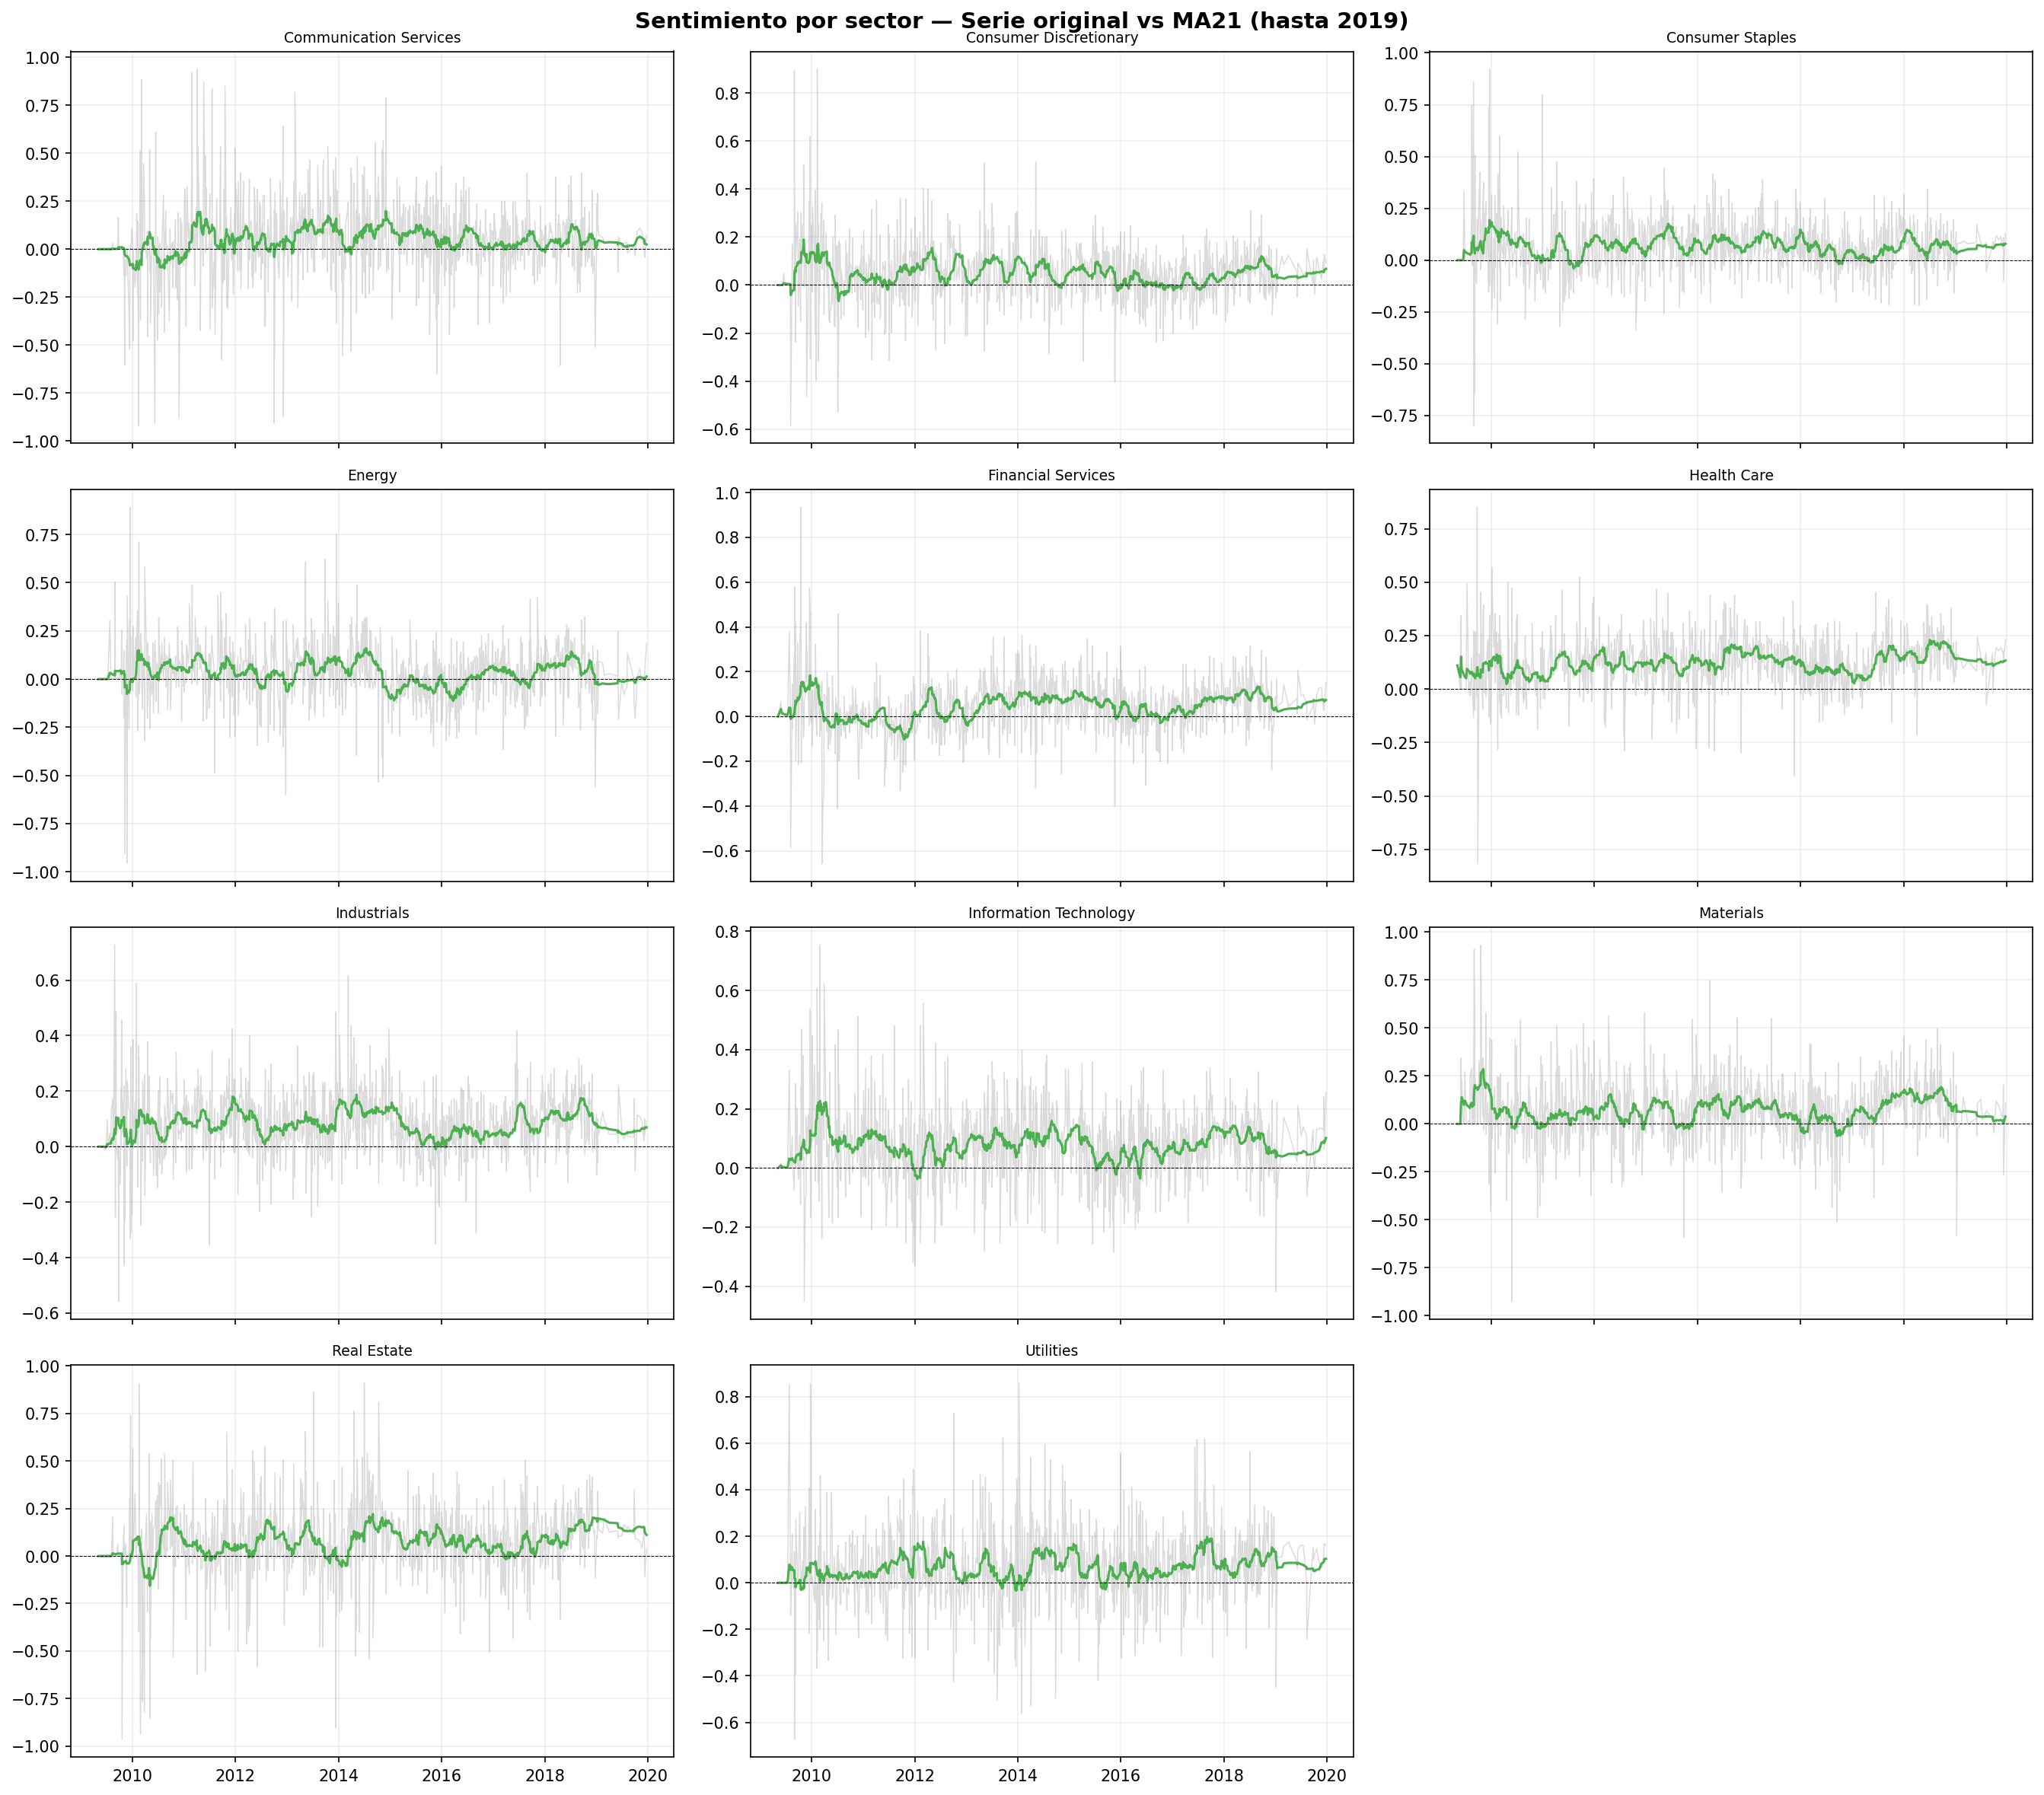
\includegraphics[width=0.95\textwidth]{figures/fig_sentiment_smoothing_summary.png}
  \caption{Raw (light) versus MA21-smoothed (dark) sector sentiment series for all 11 GICS sectors. The MA21 smoothing substantially reduces high-frequency noise while preserving medium-term sentiment trends.}
  \label{fig:sentiment-smoothing}
\end{figure}

It should be noted that this exploratory smoothing-window analysis was
conducted on an earlier development snapshot of the sentiment dataset
(covering 2009-05-08 to 2019-12-23, 1{,}073 daily observations); the final
clustering dataset used throughout the remainder of this thesis
(\Cref{sec:meth-dataset}) extends this range through February 2024. The
qualitative conclusion --- that MA21 offers the best trade-off between
noise reduction and preservation of medium-term trends --- is not
sensitive to this difference, since the smoothing window operates locally
on the time series and its relative noise-reduction properties depend on
the high-frequency statistical structure of the sentiment series rather
than on its total length.

\section{Technical Indicators}
\label{sec:meth-technical}

Nine technical indicators are computed from the daily closing price
$P_\tau$ of the S\&P 500 index. Let $r_\tau = \ln(P_\tau / P_{\tau-1})$
denote the daily log-return.

\begin{description}
  \item[Relative Strength Index (\texttt{RSI\_sp500}).] Computed using
  Wilder's exponential smoothing, implemented via an exponentially
  weighted moving average (EWM) with center-of-mass $\mathrm{com} =
  \mathrm{window} - 1 = 13$ (i.e., a 14-session RSI):
  \begin{equation}
    \label{eq:rsi}
    \mathrm{RSI}_\tau = 100 - \frac{100}{1 + RS_\tau}, \qquad
    RS_\tau = \frac{\mathrm{EWM}_{14}(\max(r_\tau, 0))}{\mathrm{EWM}_{14}(\max(-r_\tau, 0))}.
  \end{equation}

  \item[Moving-average ratios (\texttt{MA50\_ratio\_sp500},
  \texttt{MA200\_ratio\_sp500}).] The ratio of the current price to its
  50- and 200-session simple moving averages:
  \begin{equation}
    \label{eq:ma-ratio}
    \mathrm{MA}n\_\mathrm{ratio}_\tau = \frac{P_\tau}{\mathrm{SMA}_n(P)_\tau},
    \qquad n \in \{50, 200\}.
  \end{equation}
  Values above 1 indicate that the price is trading above its $n$-session
  average (an uptrend signal), and values below 1 indicate the opposite.

  \item[Momentum (\texttt{mom21\_sp500}, \texttt{mom126\_sp500}).] The
  percentage price change over the last 21 and 126 sessions
  (approximately one month and six months):
  \begin{equation}
    \label{eq:momentum}
    \mathrm{mom}n_\tau = \frac{P_\tau}{P_{\tau-n}} - 1, \qquad n \in \{21, 126\}.
  \end{equation}

  \item[Realized volatility (\texttt{vol30d\_sp500}, \texttt{vol252d\_sp500}).]
  The annualized standard deviation of log-returns over rolling windows of
  30 and 252 sessions (approximately one month and one year):
  \begin{equation}
    \label{eq:realized-vol}
    \mathrm{vol}n_\tau = \mathrm{std}\left(r_{\tau-n+1}, \dots, r_\tau\right)
    \times \sqrt{252}, \qquad n \in \{30, 252\}.
  \end{equation}

  \item[Return skewness (\texttt{skew30d\_sp500}, \texttt{skew252d\_sp500}).]
  The (Fisher-Pearson) sample skewness of log-returns over rolling windows
  of 30 and 252 sessions:
  \begin{equation}
    \label{eq:skewness}
    \mathrm{skew}n_\tau = \mathrm{skew}\left(r_{\tau-n+1}, \dots, r_\tau\right),
    \qquad n \in \{30, 252\}.
  \end{equation}
  Negative skewness indicates a distribution with a heavier left tail ---
  i.e., a higher relative likelihood of large negative returns --- which
  is a hallmark of crisis-type market dynamics.
\end{description}

These nine variables --- $\mathrm{RSI}$, two MA ratios, two momentum
measures, two realized volatilities, and two skewness measures --- form
the set \texttt{FEATURES\_TECH}, which is used directly in Model A and as
the technical component of Model B (\Cref{sec:meth-kmeans}).

\section{Clustering Dataset Construction}
\label{sec:meth-dataset}

The final clustering dataset is built by performing an \textbf{inner
merge}, on the \texttt{date} column, of (i) the wide table of sector-level
sentiment statistics (raw means and standard deviations, plus MA21-smoothed
means, for all 11 GICS sectors --- 33 sentiment columns in total) and (ii)
the table of nine technical indicators described in
\Cref{sec:meth-technical}. Technical-indicator column names are
standardized with a \texttt{\_sp500} suffix (e.g., \texttt{RSI} $\to$
\texttt{RSI\_sp500}, \texttt{mom126} $\to$ \texttt{mom126\_sp500},
\texttt{skew\_30d} $\to$ \texttt{skew30d\_sp500}) for consistency with the
sentiment column naming convention. Rows with missing values in any of
the nine technical features (which occur at the start of the series, where
the longest rolling windows --- 252 sessions --- are not yet fully
populated) are dropped.

The resulting dataset spans \textbf{2{,}009-05-08 to 2024-02-01} and
contains \textbf{1{,}132 daily observations} and \textbf{46 columns} in
total: 1 date column, 9 technical-indicator columns, 33 sentiment columns
(11 sectors $\times$ \{\texttt{avg}, \texttt{std}, \texttt{avg\_smooth}\}),
and (after clustering) the cluster-label columns described in the next
section.

\section{K-Means Clustering: Models A, B and C}
\label{sec:meth-kmeans}

\subsection{Selection of the Number of Clusters}

For each of the three feature configurations described below, the
\textit{K-Means} algorithm (\Cref{eq:soa-kmeans-objective}) is run for
$K \in \{2, \dots, 7\}$ with \texttt{k-means++} initialization, 10
independent initializations (\texttt{n\_init=10}) and
\texttt{random\_state=42} for reproducibility, after standardizing all
input features to zero mean and unit variance
(\texttt{StandardScaler}). For each $K$, the inertia (within-cluster sum
of squares, \Cref{eq:soa-kmeans-objective}) and the silhouette coefficient
(\Cref{eq:soa-silhouette}) are recorded. \Cref{fig:elbow-modelA,fig:elbow-modelB,fig:elbow-modelC}
show the resulting elbow/silhouette curves for Models A, B and C,
respectively. In all three cases, $K=3$ is selected: it lies at (or
immediately after) the ``elbow'' of the inertia curve, corresponds to a
local maximum or plateau of the silhouette curve, and --- crucially for
the interpretability goals of this thesis --- maps naturally onto the
\emph{Bull / Bear / Crisis} trichotomy discussed in
\Cref{sec:soa-kmeans}. A common value of $K=3$ across all three models
also ensures that Models A, B and C remain directly comparable.

\begin{figure}[H]
  \centering
  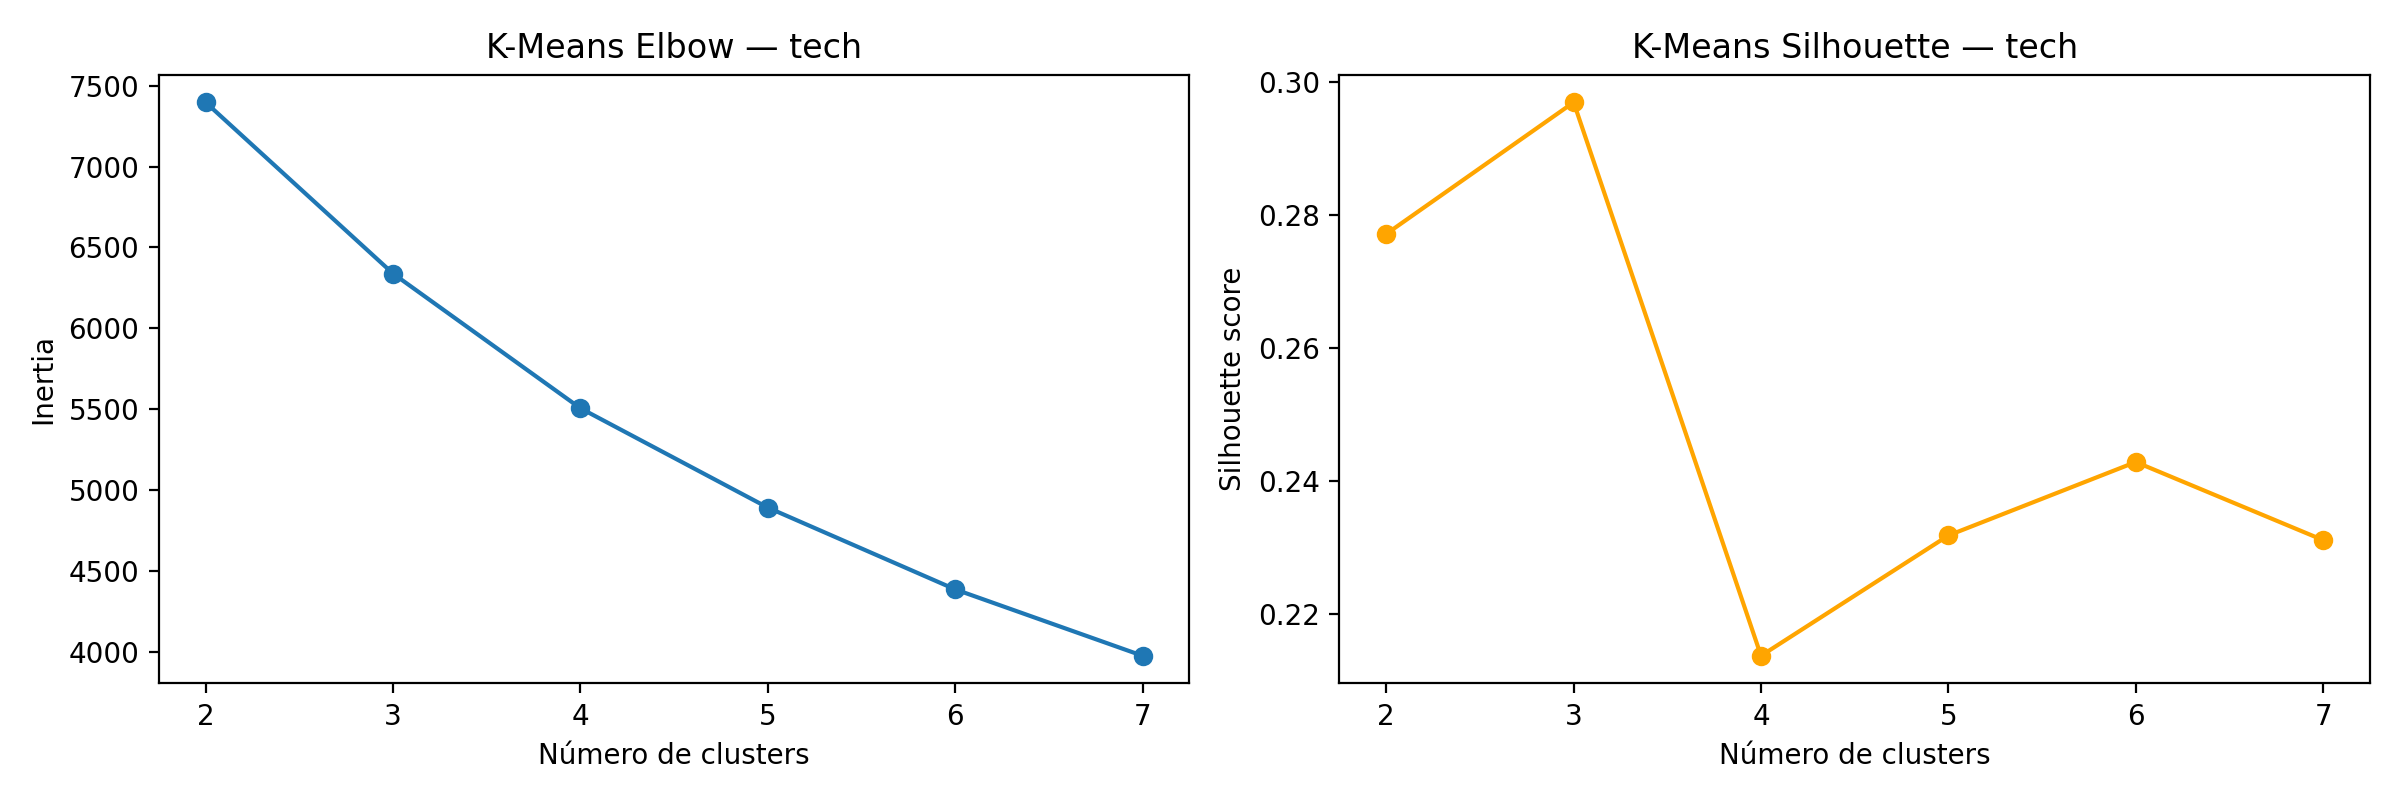
\includegraphics[width=0.95\textwidth]{figures/fig_elbow_modelA.png}
  \caption{Elbow (inertia) and silhouette curves for $K \in \{2,\dots,7\}$, Model A (technical indicators only).}
  \label{fig:elbow-modelA}
\end{figure}

\begin{figure}[H]
  \centering
  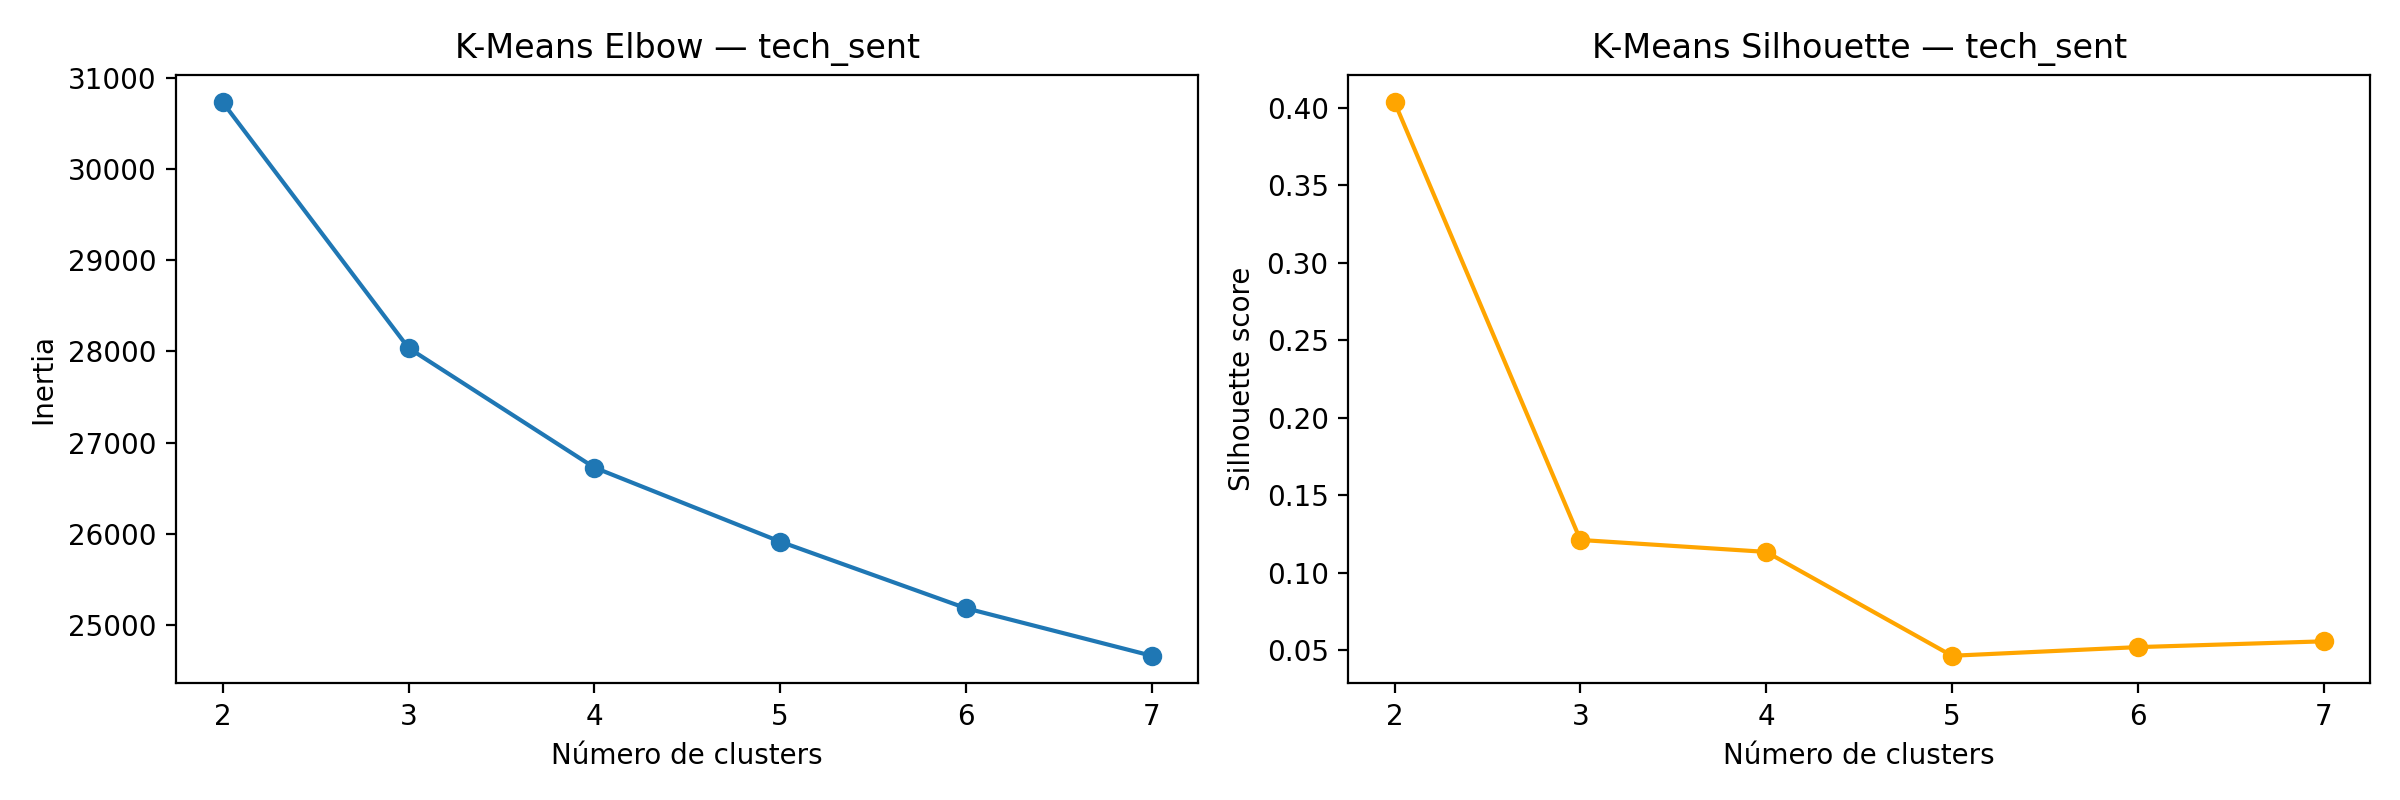
\includegraphics[width=0.95\textwidth]{figures/fig_elbow_modelB.png}
  \caption{Elbow (inertia) and silhouette curves for $K \in \{2,\dots,7\}$, Model B (technical indicators + raw sector sentiment).}
  \label{fig:elbow-modelB}
\end{figure}

\begin{figure}[H]
  \centering
  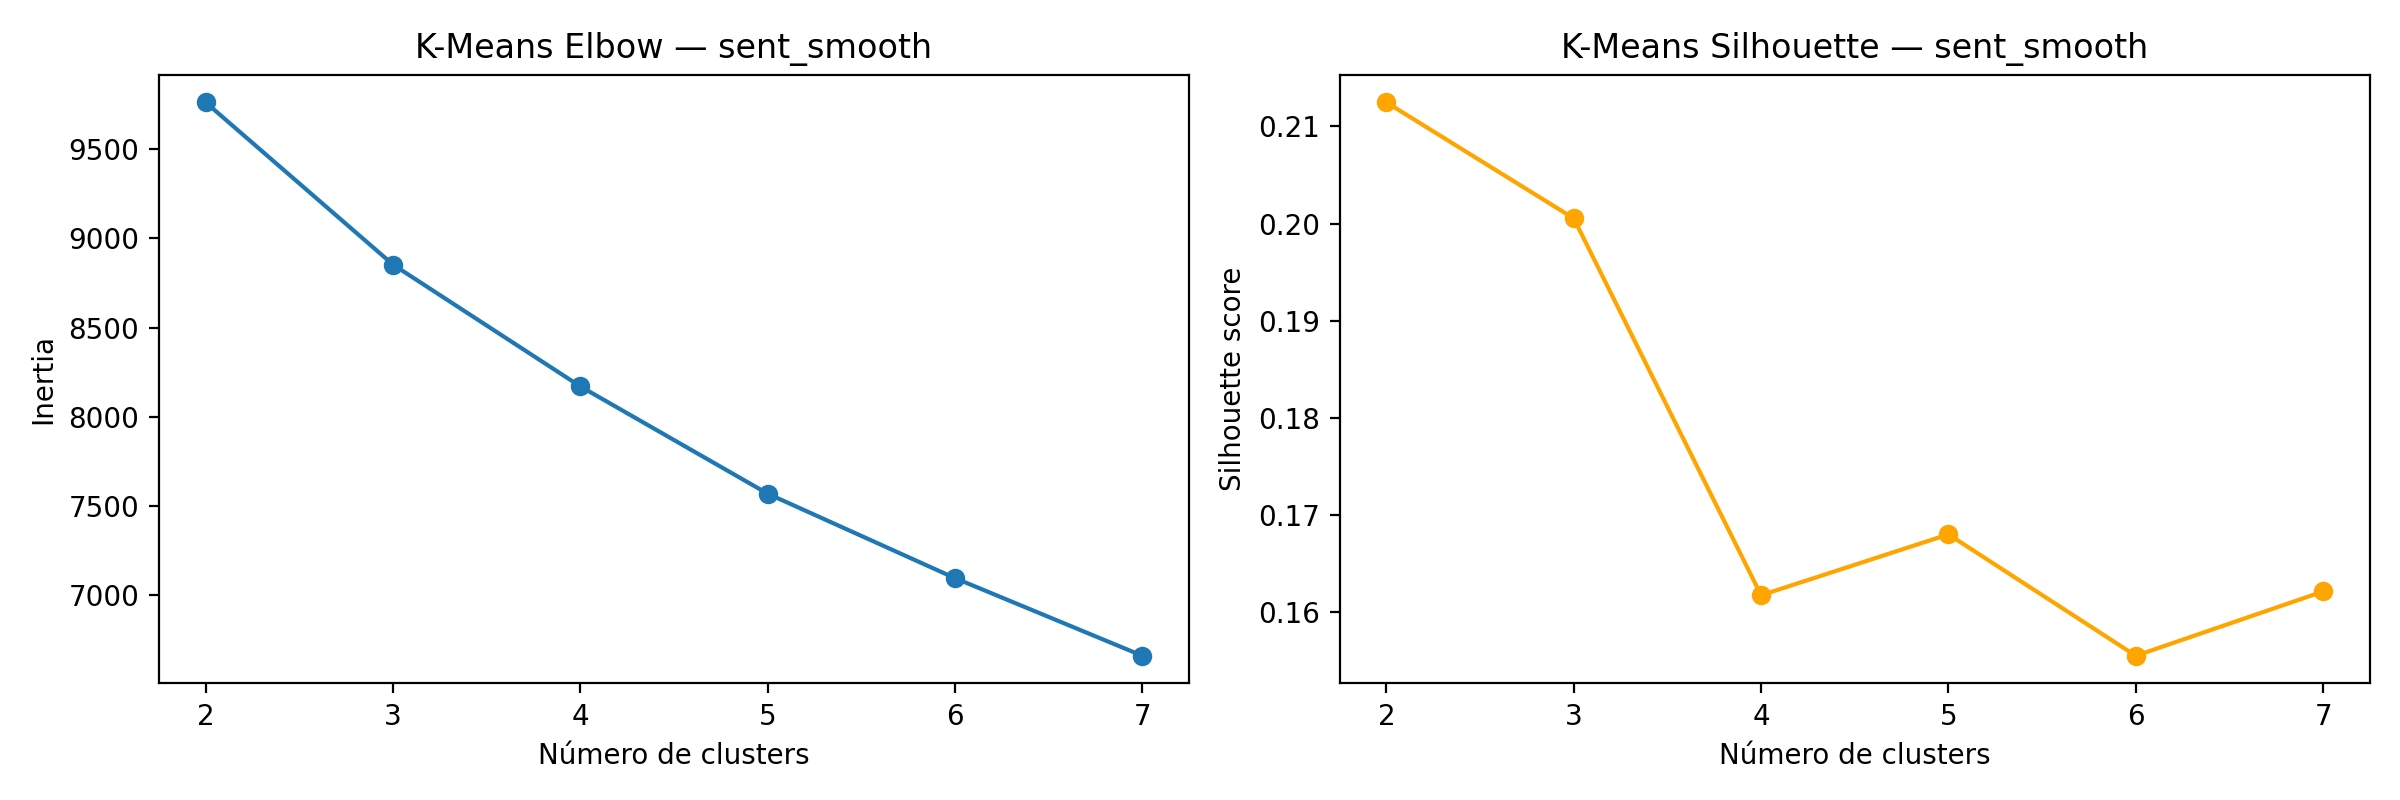
\includegraphics[width=0.95\textwidth]{figures/fig_elbow_modelC.png}
  \caption{Elbow (inertia) and silhouette curves for $K \in \{2,\dots,7\}$, Model C (smoothed sector sentiment only).}
  \label{fig:elbow-modelC}
\end{figure}

\subsection{Model A: Technical Indicators Only}

\textbf{Model A} uses exclusively the $d=9$ features in
\texttt{FEATURES\_TECH} (\Cref{sec:meth-technical}). This model serves as
the \emph{baseline}: it represents the ``classical'' approach to
clustering-based regime detection, using only price-derived information.
The resulting cluster labels are stored in the column
\texttt{kmeans\_tech}.

\subsection{Model B: Technical Indicators + Raw Sector Sentiment}

\textbf{Model B} augments the 9 technical features with the $22$ raw
(non-smoothed) sentiment columns --- \texttt{sentiment\_avg\_<sector>} and
\texttt{sentiment\_std\_<sector>} for each of the 11 GICS sectors --- for
a total of $d = 9 + 22 = 31$ features. This is the model that most
directly addresses the central research question of this thesis: does
adding contemporaneous sector-level sentiment information to the
technical baseline change the resulting regime partition, and if so, does
it do so in a way that is economically meaningful? The resulting cluster
labels are stored in the column \texttt{kmeans\_tech\_sent}.

\subsection{Model C: Smoothed Sector Sentiment Only}

\textbf{Model C} uses exclusively the $d=11$ MA21-smoothed sentiment means
(\texttt{sentiment\_avg\_<sector>\_smooth}, \Cref{sec:meth-smoothing}), with
no technical indicators at all. This model serves as a \emph{stress test}
of the sentiment signal in isolation: if sentiment alone were sufficient
to recover regimes with technical (price/volatility) characteristics
similar to those of Models A and B, this would suggest that sentiment is a
strong \emph{leading} indicator of the technical regime. Conversely, if
Model C's clusters show little technical differentiation, this indicates
that sentiment, while potentially informative as a complement
(cf.\ Model B), is not on its own a sufficient basis for regime detection.
The resulting cluster labels are stored in the column
\texttt{kmeans\_sent\_smooth}.

\Cref{tab:model-summary} summarizes the three models.

\begin{table}[H]
\centering
\caption{Summary of the three K-Means model configurations.}
\label{tab:model-summary}
\begin{tabular}{lllc}
\toprule
\textbf{Model} & \textbf{Feature set} & \textbf{Column} & \textbf{$d$} \\
\midrule
A & Technical indicators only & \texttt{kmeans\_tech} & 9 \\
B & Technical + raw sector sentiment (avg + std) & \texttt{kmeans\_tech\_sent} & 31 \\
C & Smoothed (MA21) sector sentiment only & \texttt{kmeans\_sent\_smooth} & 11 \\
\bottomrule
\end{tabular}
\end{table}

\section{Gaussian Hidden Markov Model: A Secondary Comparison Method}
\label{sec:meth-hmm}

To complement the \textit{K-Means} models with a method that explicitly
accounts for temporal transition dynamics
(\Cref{sec:soa-hmm}), a \textbf{Gaussian Hidden Markov Model} is fitted
using the \texttt{hmmlearn} implementation, with the following
configuration:

\begin{itemize}
  \item Number of hidden states: $K=3$ (matching the \textit{K-Means}
  models for comparability).
  \item Emission distributions: full covariance Gaussians
  (\texttt{covariance\_type="full"}), allowing each state to have its own
  unrestricted covariance structure across features.
  \item Optimization: Baum-Welch (EM) algorithm, \texttt{n\_iter=1000}
  maximum iterations.
  \item Numerical stability: a minimum covariance floor
  \texttt{min\_covar=1e-3} is imposed to avoid degenerate (near-singular)
  covariance estimates.
  \item Reproducibility: \texttt{random\_state=42}.
\end{itemize}

The HMM is fitted separately on the standardized feature sets
corresponding to \textbf{Model A} (the 9 technical features,
\texttt{hmm\_tech}) and \textbf{Model B} (the 31 technical + raw-sentiment
features, \texttt{hmm\_tech\_sent}), using the same
\texttt{StandardScaler}-transformed inputs as the corresponding
\textit{K-Means} model. After fitting, the most likely state sequence is
obtained via \texttt{hmm.predict()} (Viterbi decoding), yielding a state
label $h_\tau \in \{0,1,2\}$ for each trading day $\tau$.

Because $K$ is identical and the input feature sets are identical (after
standardization) to those of Models A and B, the HMM provides a
\emph{like-for-like} comparison point: any differences in the resulting
partitions (cluster sizes, temporal persistence, and --- most importantly
for this thesis --- economic differentiation across states, see
\Cref{ch:results}) can be attributed to the modeling choice (static
clustering vs. Markov-switching with explicit transition dynamics) rather
than to differences in the underlying data.

\section{Regime Labeling Methodology}
\label{sec:meth-labeling}

The raw cluster/state indices produced by \textit{K-Means} and the HMM
(integers $0,1,2$, with no inherent ordering or meaning) are mapped to the
economically meaningful labels \emph{Bull}, \emph{Bear} and
\emph{Crisis} by inspecting the \textbf{centroids} (cluster means) of the
nine technical features (\Cref{eq:rsi}--\Cref{eq:skewness}) for each
cluster. The labeling heuristic is as follows:

\begin{itemize}
  \item The cluster with \textbf{positive momentum} (\texttt{mom21},
  \texttt{mom126} $> 0$), \texttt{RSI} above 50, moving-average ratios
  above 1, and \emph{moderate} volatility is labeled \textbf{Bull}.
  \item The cluster with \textbf{negative (or near-zero) momentum},
  \texttt{RSI} below 50, moving-average ratios below or near 1, and
  elevated volatility is labeled \textbf{Bear}.
  \item The cluster with the \textbf{highest realized volatility}
  (particularly \texttt{vol252d}) and the most extreme (most negative)
  return skewness, often combined with a strong rebound in 126-session
  momentum, is labeled \textbf{Crisis}.
\end{itemize}

\Cref{tab:centroids-modelA} and \Cref{tab:centroids-modelB} report the
resulting centroids and cluster sizes for Models A and B (after applying
\texttt{StandardScaler} inversely, i.e., in the original units of each
feature), confirming that this heuristic assigns cluster index $0 \to$
Bull, $1 \to$ Bear and $2 \to$ Crisis consistently for both models.

\begin{table}[H]
\centering
\caption{Model A (technical-only): cluster centroids (mean feature values) and cluster sizes, $n=1{,}132$ observations.}
\label{tab:centroids-modelA}
\small
\begin{tabular}{lrrr}
\toprule
\textbf{Feature} & \textbf{Cluster 0 (Bull)} & \textbf{Cluster 1 (Bear)} & \textbf{Cluster 2 (Crisis)} \\
\midrule
RSI\_sp500          & 60.34 & 42.57 & 59.25 \\
MA50\_ratio\_sp500  & 1.0229 & 0.9739 & 1.0392 \\
MA200\_ratio\_sp500 & 1.0620 & 0.9877 & 1.1337 \\
mom21\_sp500        & 0.0227 & $-$0.0297 & 0.0281 \\
mom126\_sp500       & 0.0793 & $-$0.0075 & 0.2373 \\
vol30d\_sp500       & 0.1120 & 0.2005 & 0.1765 \\
vol252d\_sp500      & 0.1405 & 0.1670 & 0.3718 \\
skew30d\_sp500      & $-$0.1417 & $-$0.2704 & $-$0.4073 \\
skew252d\_sp500     & $-$0.3879 & $-$0.5259 & $-$0.2129 \\
\midrule
\textbf{$n$ (days)}  & \textbf{745} & \textbf{317} & \textbf{70} \\
\textbf{Share}       & 65.8\% & 28.0\% & 6.2\% \\
\bottomrule
\end{tabular}
\end{table}

\begin{table}[H]
\centering
\caption{Model B (technical + raw sentiment): cluster centroids (technical features only, for comparability with Model A) and cluster sizes, $n=1{,}132$ observations.}
\label{tab:centroids-modelB}
\small
\begin{tabular}{lrrr}
\toprule
\textbf{Feature} & \textbf{Cluster 0 (Bull)} & \textbf{Cluster 1 (Bear)} & \textbf{Cluster 2 (Crisis)} \\
\midrule
RSI\_sp500          & 60.50 & 43.34 & 60.11 \\
MA50\_ratio\_sp500  & 1.0235 & 0.9766 & 1.0374 \\
MA200\_ratio\_sp500 & 1.0647 & 0.9905 & 1.1190 \\
mom21\_sp500        & 0.0226 & $-$0.0265 & 0.0315 \\
mom126\_sp500       & 0.0841 & $-$0.0036 & 0.1997 \\
vol30d\_sp500       & 0.1110 & 0.1967 & 0.1734 \\
vol252d\_sp500      & 0.1417 & 0.1682 & 0.3438 \\
skew30d\_sp500      & $-$0.1430 & $-$0.2603 & $-$0.3975 \\
skew252d\_sp500     & $-$0.4137 & $-$0.4842 & $-$0.1016 \\
\midrule
\textbf{$n$ (days)}  & \textbf{720} & \textbf{342} & \textbf{70} \\
\textbf{Share}       & 63.6\% & 30.2\% & 6.2\% \\
\bottomrule
\end{tabular}
\end{table}

For \textbf{Model C}, the same $0 \to$ Bull, $1 \to$ Bear, $2 \to$ Crisis
mapping (based on the relative ordering of the smoothed-sentiment
centroids) is applied for consistency with Models A and B in the
economic-validation pipeline. However, as discussed in
\Cref{sec:results-modelC} of \Cref{ch:results}, when the \emph{technical}
feature centroids are computed for Model C's clusters (i.e., projecting
Model C's sentiment-only partition back onto the technical feature space),
the three clusters turn out to be \textbf{nearly indistinguishable} ---
e.g., \texttt{MA50\_ratio\_sp500} ranges only from $1.0086$ to $1.0134$
across Model C's three clusters, compared to a range of roughly $0.97$ to
$1.04$ for Models A and B. This observation is central to the discussion
of Model C as a methodologically informative negative result.

\section{Economic Validation Framework}
\label{sec:meth-validation}

The final stage of the methodology evaluates the \emph{economic} content
of the detected regimes, independently of the purely statistical
clustering metrics discussed in \Cref{ch:results}.

\subsection{Sector-Level Equally-Weighted Price Indices}

For each GICS sector $g$, an equally-weighted (EW) daily return series is
constructed from the historical S\&P 500 constituents belonging to sector
$g$ (\Cref{sec:meth-gics}). Daily close-to-close returns
$r_{\tau}^{(j)}$ are computed for every ticker $j$ in sector $g$ (using
\texttt{yfinance}-sourced, dividend- and split-adjusted closing prices,
cached locally as Parquet), and the sector return on day $\tau$ is defined
as the simple cross-sectional average:

\begin{equation}
  \label{eq:sector-return}
  R_{\tau,g} = \frac{1}{|\mathcal{J}_g|} \sum_{j \in \mathcal{J}_g} r_\tau^{(j)},
\end{equation}

where $\mathcal{J}_g$ is the set of tickers historically assigned to
sector $g$ that have available price data on day $\tau$.

\subsection{Regime Assignment to the Daily Price Calendar}

The cluster/state labels produced by Models A, B, C and the HMM are
defined on the 1{,}132-observation clustering dataset
(\Cref{sec:meth-dataset}), which does not necessarily cover every trading
day in the 2009--2024 sample with the same density as the daily price
calendar used for the sector return series. To align the two, the
cluster-label series is reindexed onto the full daily price calendar and
\textbf{forward-filled} (each day is assigned the most recently known
regime label), under the assumption that a detected regime remains in
effect until a new observation indicates otherwise. After reindexing, the
total number of (sector, regime)-labeled days is $3{,}695$ for every
model, distributed across the three regimes as shown in
\Cref{ch:results}.

\subsection{Economic Metrics}

For every combination of GICS sector $g$ and regime $\rho \in
\{\text{Bull}, \text{Bear}, \text{Crisis}\}$, let
$\{R_{\tau,g}\}_{\tau \in \mathcal{D}_{g,\rho}}$ denote the sector returns
on the subset of days $\mathcal{D}_{g,\rho}$ assigned to regime $\rho$,
with $n = |\mathcal{D}_{g,\rho}|$. The following metrics are computed
(combinations with $n < 10$ are excluded as statistically unreliable):

\begin{description}
  \item[Annualized return.] Computed from the total compounded return over
  the (non-contiguous) set of days assigned to the regime, annualized
  assuming $252$ trading days per year:
  \begin{equation}
    \label{eq:ann-return}
    \mu_{g,\rho} = \left(1 + \prod_{\tau \in \mathcal{D}_{g,\rho}}
    (1 + R_{\tau,g}) - 1\right)^{252/n} - 1.
  \end{equation}

  \item[Annualized volatility.]
  \begin{equation}
    \label{eq:ann-vol}
    \sigma_{g,\rho} = \mathrm{std}\left(\{R_{\tau,g}\}_{\tau \in
    \mathcal{D}_{g,\rho}}\right) \times \sqrt{252}.
  \end{equation}

  \item[Sharpe ratio.] With risk-free rate $r_f = 2\%$:
  \begin{equation}
    \label{eq:sharpe}
    \mathrm{Sharpe}_{g,\rho} = \frac{\mu_{g,\rho} - r_f}{\sigma_{g,\rho}}.
  \end{equation}

  \item[Maximum drawdown.] Computed on the cumulative return series
  $\mathrm{Cum}_\tau = \prod_{\tau' \le \tau, \tau' \in
  \mathcal{D}_{g,\rho}} (1 + R_{\tau',g})$ \emph{restricted to the days
  assigned to the regime} (i.e., treating the regime's days as if they
  were contiguous):
  \begin{equation}
    \label{eq:max-dd}
    \mathrm{MaxDD}_{g,\rho} = \min_\tau \frac{\mathrm{Cum}_\tau -
    \max_{\tau' \le \tau} \mathrm{Cum}_{\tau'}}{\max_{\tau' \le \tau}
    \mathrm{Cum}_{\tau'}}.
  \end{equation}
  Because the days in $\mathcal{D}_{g,\rho}$ are generally
  \emph{non-contiguous} in calendar time, $\mathrm{MaxDD}_{g,\rho}$ should
  be interpreted as a measure of the worst \emph{within-regime} compounded
  loss sequence, not as the drawdown of a literal buy-and-hold strategy.

  \item[Percentage of positive days.]
  $\mathrm{PctPos}_{g,\rho} = \frac{1}{n}\left|\{\tau \in
  \mathcal{D}_{g,\rho} : R_{\tau,g} > 0\}\right|$.

  \item[Best/worst single-day return.]
  $\mathrm{Best}_{g,\rho} = \max_{\tau \in \mathcal{D}_{g,\rho}} R_{\tau,g}$
  and $\mathrm{Worst}_{g,\rho} = \min_{\tau \in \mathcal{D}_{g,\rho}}
  R_{\tau,g}$. These extreme-value statistics are particularly informative
  for the \emph{Crisis} regime, where they capture the magnitude of the
  largest single-day moves (in either direction) that the regime is
  associated with.
\end{description}

For each metric, a heatmap with GICS sectors on the rows and regimes
(\emph{Bull}, \emph{Bear}, \emph{Crisis}) on the columns is generated,
providing a compact visual summary of how each regime manifests
economically across all 11 sectors simultaneously. These heatmaps, for
Models A, B and C, are presented and discussed in \Cref{ch:results}, with
the complete numerical tables reproduced in Annex~B.

\chapter{Results}
\label{ch:results}

This chapter presents the results obtained by applying the methodology
described in \Cref{ch:methodology}. \Cref{sec:results-silhouette}
compares the internal clustering quality of Models A, B and C.
\Cref{sec:results-pca} presents PCA-based visualizations of the
clustering structure. \Cref{sec:results-correlation} analyzes the
correlation structure of the input features. \Cref{sec:results-importance}
reports feature importance for Model B.
\Cref{sec:results-regimes} examines the temporal distribution of the
detected regimes. \Cref{sec:results-econ-overall} and
\Cref{sec:results-econ-sector} present the economic validation results at
the market and sector levels, respectively. \Cref{sec:results-modelC}
discusses Model C as a negative result. \Cref{sec:results-hmm} compares
\textit{K-Means} with the Gaussian HMM. Finally,
\Cref{sec:results-summary} synthesizes the key findings.

\section{Internal Validation: Silhouette Comparison}
\label{sec:results-silhouette}

\Cref{tab:silhouette-comparison} reports the silhouette coefficient
(\Cref{eq:soa-silhouette}) for Models A, B and C, computed in two
different feature spaces: (i) each model's own (standardized) feature
space, as used during training, and (ii) a \textbf{common PCA space},
obtained by applying PCA to the union of the 9 technical features and the
11 MA21-smoothed sentiment features (20 features in total, standardized),
and retaining the first 9 principal components, which jointly explain
82.0\% of the total variance.

\begin{table}[H]
\centering
\caption{Silhouette coefficient for Models A, B and C, in each model's own feature space and in a common PCA space (9 components, 82.0\% explained variance).}
\label{tab:silhouette-comparison}
\begin{tabular}{lcc}
\toprule
\textbf{Model} & \textbf{Silhouette (own space)} & \textbf{Silhouette (common PCA space)} \\
\midrule
A -- Technical only             & 0.2969 & 0.1928 \\
B -- Technical + raw sentiment  & 0.1213 & 0.1778 \\
C -- Smoothed sentiment only    & 0.2005 & 0.1623 \\
\bottomrule
\end{tabular}
\end{table}

Two observations follow from \Cref{tab:silhouette-comparison}. First, when
each model is evaluated in its \emph{own} feature space, Model A
(technical only, $d=9$) achieves by far the highest silhouette
(0.2969), while Model B (technical + raw sentiment, $d=31$) achieves the
lowest (0.1213). This is unsurprising: adding 22 additional sentiment
dimensions to the 9 technical dimensions dilutes the relative contribution
of the technical features --- which are the features most strongly
associated with the cluster structure, as confirmed by the feature
importance analysis in \Cref{sec:results-importance} --- to the Euclidean
distances on which both \textit{K-Means} and the silhouette coefficient
are based. A higher-dimensional space with many comparatively
``noisy'' dimensions (the raw, day-to-day sentiment columns) tends to
produce less cohesive clusters in absolute terms.

Second, when the three models are projected into the \textbf{same} common
PCA space --- which is necessary for a fair, apples-to-apples comparison,
since silhouette values computed in feature spaces of different
dimensionality and composition are not directly comparable --- the
ranking becomes $A$ (0.1928) $>$ $B$ (0.1778) $>$ $C$ (0.1623). Model A
retains the best cluster cohesion, but the gap to Model B narrows
considerably (from $0.2969 - 0.1213 = 0.1756$ in each model's own space,
to $0.1928 - 0.1778 = 0.0150$ in the common space). This indicates that,
once the comparison is placed on equal footing, the technical+sentiment
partition (Model B) is only marginally less cohesive, in a purely
statistical sense, than the technical-only partition (Model A). Model C
falls in between the two in its own space, but ranks last in the common
PCA space, foreshadowing the negative result discussed in
\Cref{sec:results-modelC}: a partition based purely on smoothed sentiment
does not align well with the principal directions of variation of the
technical+sentiment feature space.

\Cref{fig:silhouette-pca-comparison} shows the silhouette comparison
graphically, and \Cref{fig:silhouette-scree} shows the PCA scree plot
(cumulative explained variance) used to determine the 9-component common
space.

\begin{figure}[H]
  \centering
  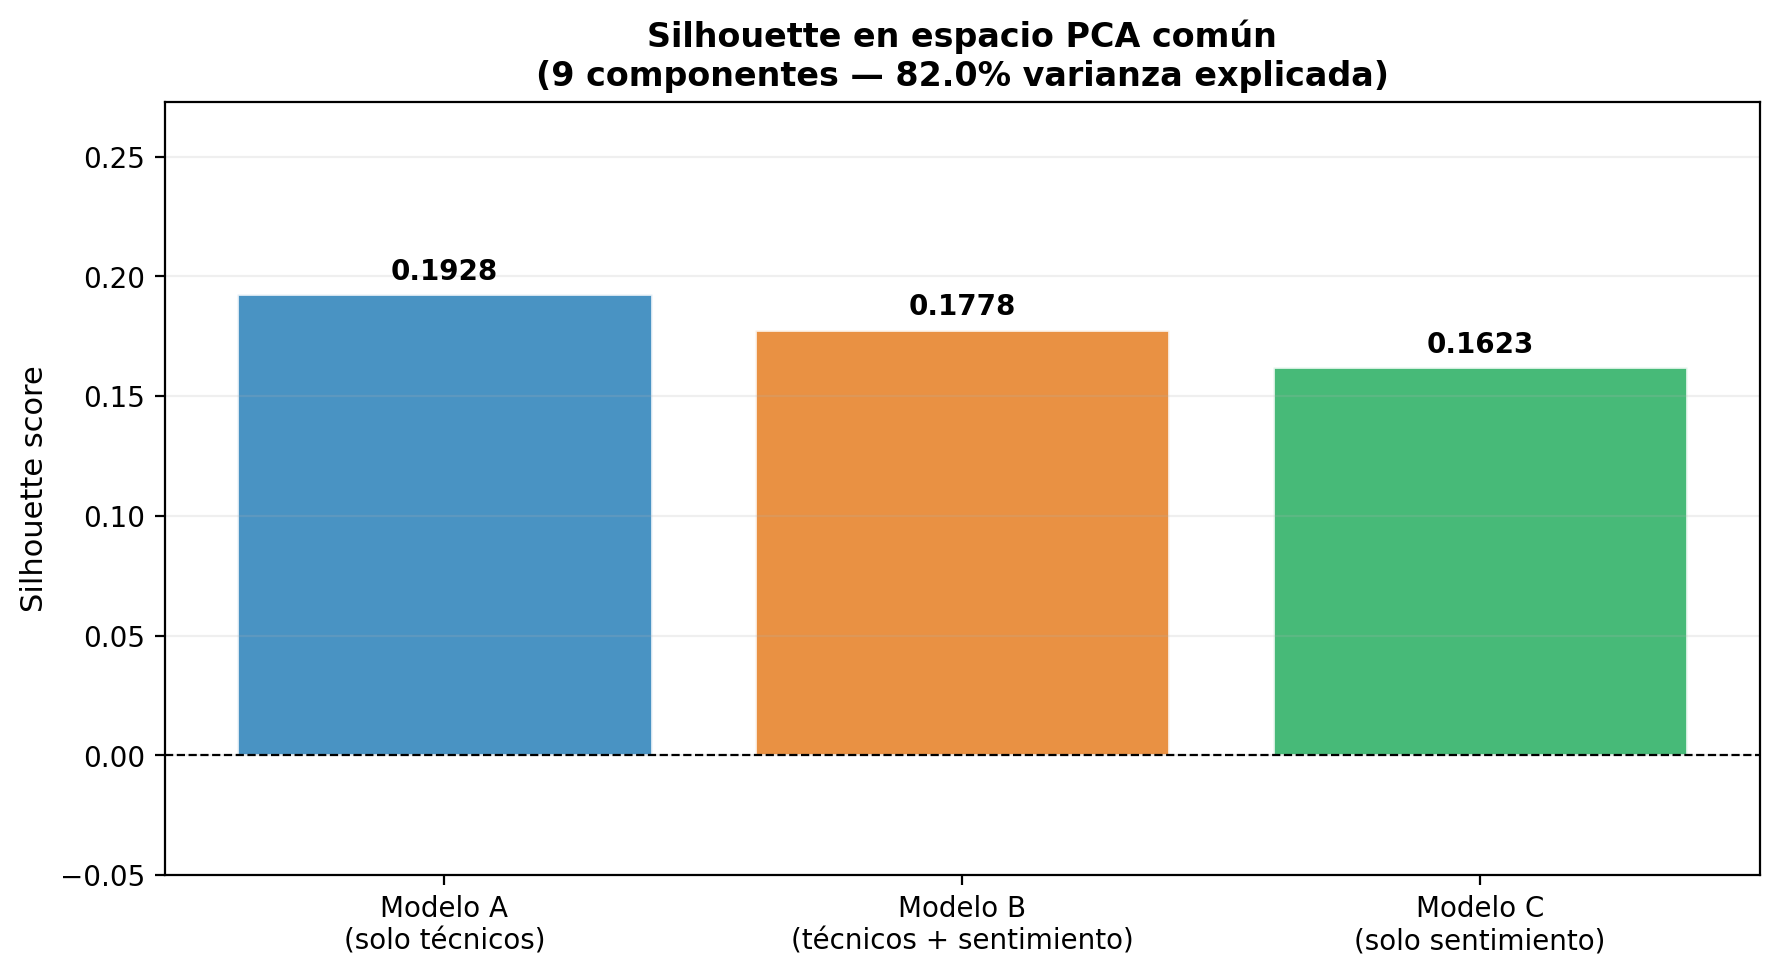
\includegraphics[width=0.85\textwidth]{figures/fig_silhouette_pca_comparison.png}
  \caption{Silhouette coefficient for Models A, B and C, computed in the common 9-component PCA space (82.0\% explained variance).}
  \label{fig:silhouette-pca-comparison}
\end{figure}

\begin{figure}[H]
  \centering
  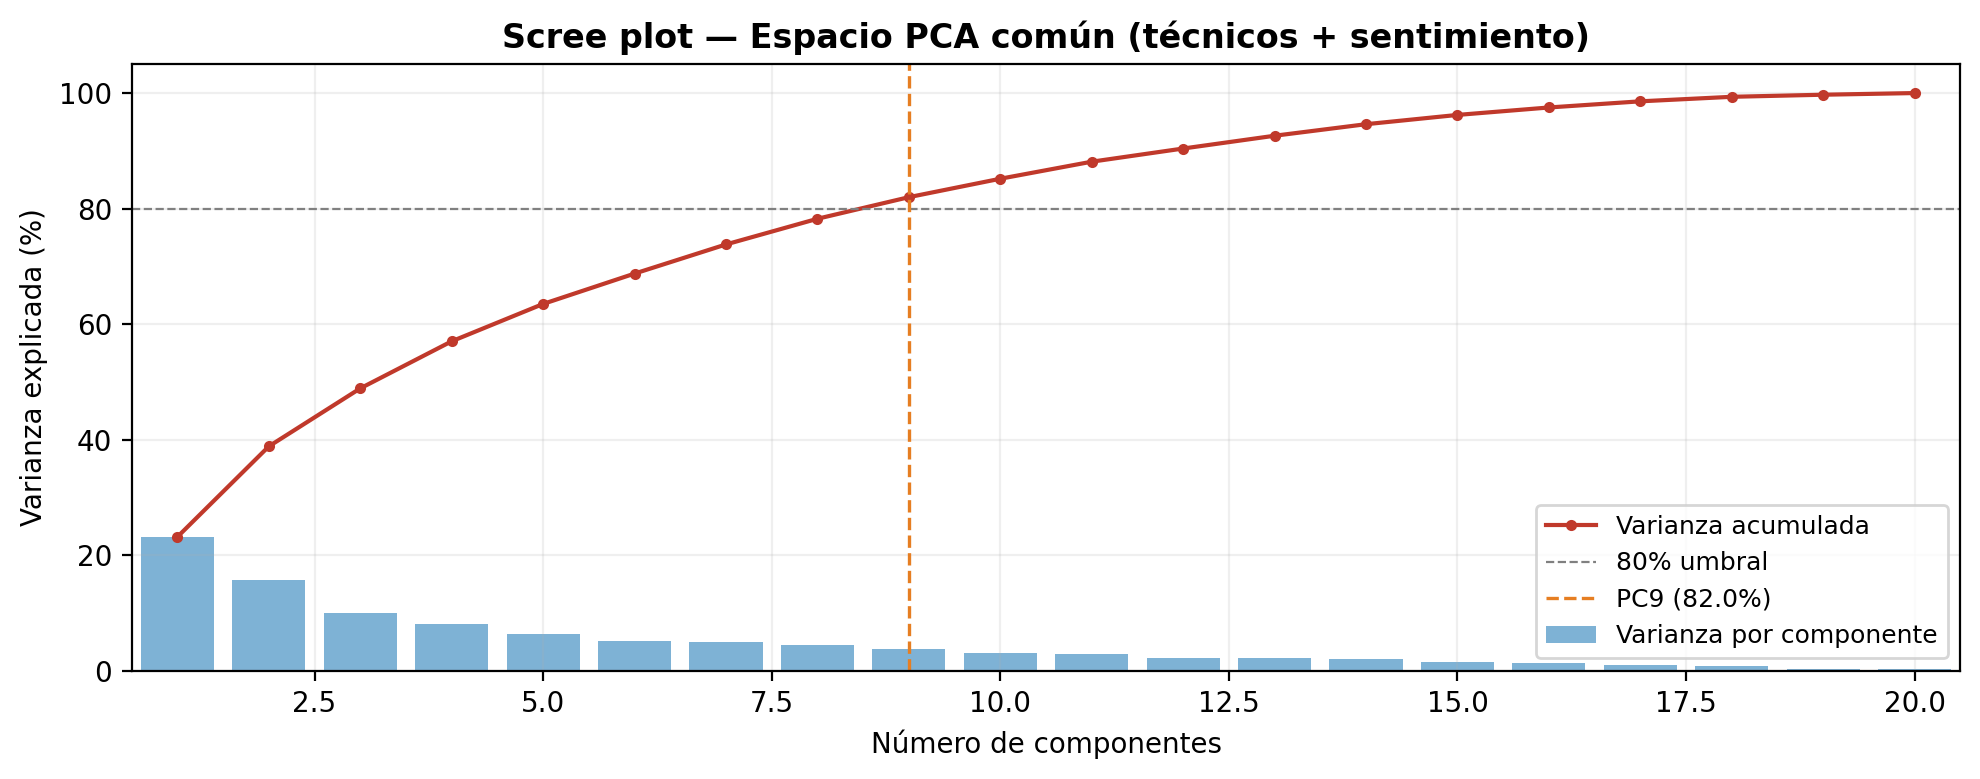
\includegraphics[width=0.85\textwidth]{figures/fig_silhouette_scree.png}
  \caption{Scree plot (cumulative explained variance) for the PCA decomposition of the 20-feature space (9 technical + 11 smoothed sentiment features) used to construct the common comparison space.}
  \label{fig:silhouette-scree}
\end{figure}

\section{PCA Visualizations}
\label{sec:results-pca}

To visualize the cluster structure in two dimensions,
\Cref{fig:pca-modelA} and \Cref{fig:pca-modelB} show, for Models A and B
respectively, a three-panel figure consisting of (i) a 2D scatter plot of
the first two principal components, colored by regime label
(\emph{Bull} in green, \emph{Bear} in red, \emph{Crisis} in orange,
following the color convention $\{0:\texttt{\#0D7A3E}, 1:\texttt{\#C0392B},
2:\texttt{\#E67E22}\}$), (ii) the loadings of the original features on the
first two principal components, and (iii) the cumulative explained
variance (scree plot).

For Model A, PCA is applied to the 9 standardized technical features:
PC1 explains 43.7\% of the variance and PC2 an additional 15.8\%
(59.5\% jointly), and 4 components are required to reach 80\% of the
total variance. For Model B, to obtain a visualization that remains
interpretable while still reflecting the sentiment dimension, PCA is
applied to the 20-feature space consisting of the 9 technical features
plus the 11 MA21-\emph{smoothed} sentiment features (rather than the full
31-feature raw space used for clustering itself): PC1 explains 23.2\% and
PC2 an additional 15.7\% (38.9\% jointly), with 9 components required to
reach 80\% of the variance --- consistent with the common PCA space used
in \Cref{sec:results-silhouette}.

\begin{figure}[H]
  \centering
  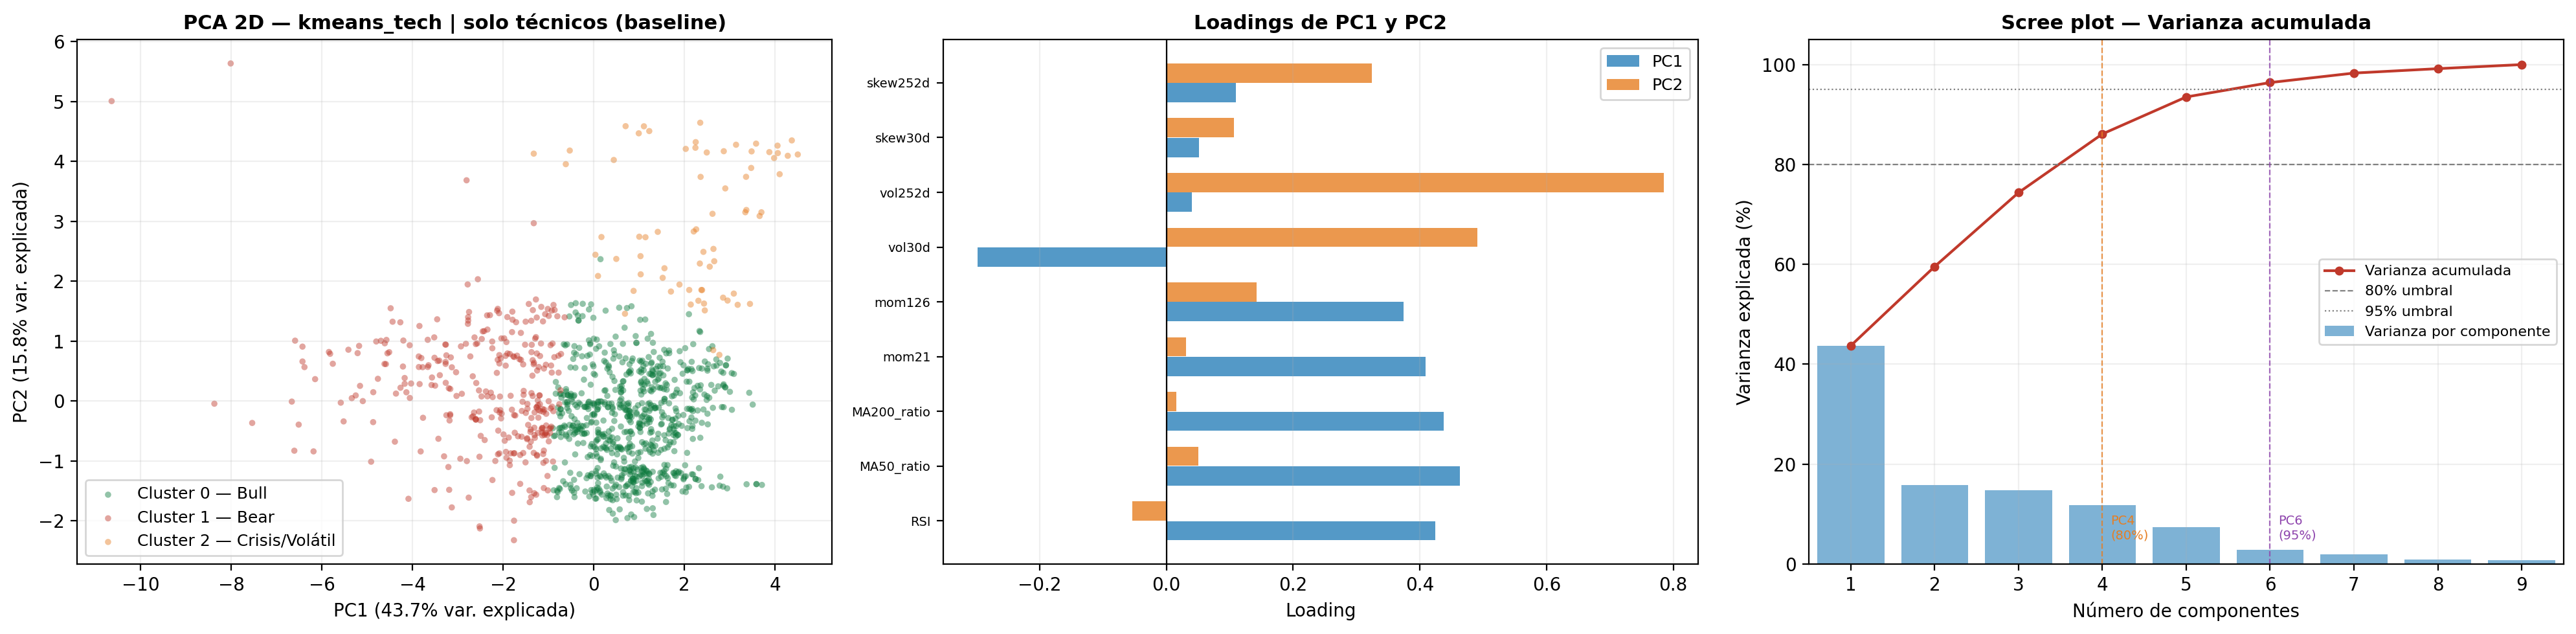
\includegraphics[width=\textwidth]{figures/fig_pca_modelA.png}
  \caption{Model A (technical only): PCA scatter plot of regimes (left), feature loadings on PC1/PC2 (center), and cumulative explained variance (right). PC1 (43.7\%) is dominated by volatility and RSI/momentum, separating the high-volatility \emph{Crisis} regime (orange) from the \emph{Bull} (green) and \emph{Bear} (red) regimes.}
  \label{fig:pca-modelA}
\end{figure}

\begin{figure}[H]
  \centering
  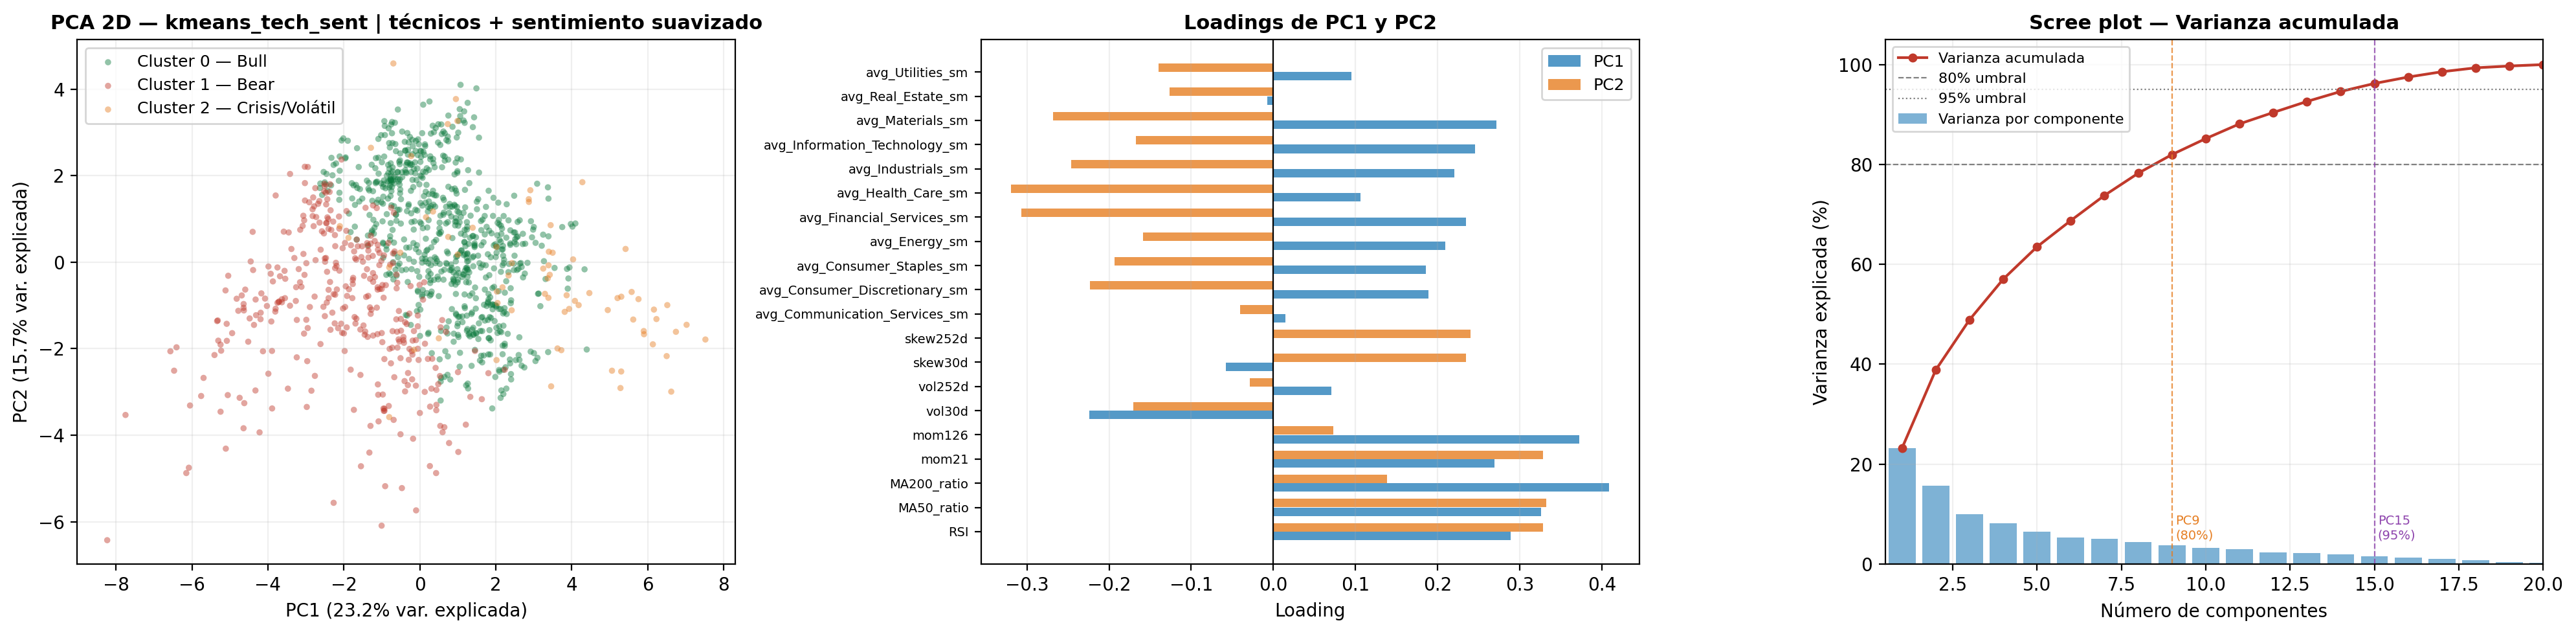
\includegraphics[width=\textwidth]{figures/fig_pca_modelB.png}
  \caption{Model B (technical + sentiment): PCA scatter plot of regimes (left; PCA computed on technical + MA21-smoothed sentiment features for visualization), feature loadings on PC1/PC2 (center), and cumulative explained variance (right).}
  \label{fig:pca-modelB}
\end{figure}

In both figures, the \emph{Crisis} regime (orange, $n=70$ in both Models A
and B) appears as a comparatively small, visually distinct cloud of
points located towards the high-volatility extreme of PC1, consistent
with its centroid profile (\Cref{tab:centroids-modelA,tab:centroids-modelB}):
substantially higher \texttt{vol252d\_sp500} than the other two regimes.
The \emph{Bull} (green) and \emph{Bear} (red) regimes show greater overlap
along PC2, reflecting the smaller relative differences in
\texttt{vol30d\_sp500} and \texttt{skew30d\_sp500} between these two
regimes compared to the gap to \emph{Crisis}.

\section{Correlation Analysis}
\label{sec:results-correlation}

\Cref{fig:correlation-modelA} and \Cref{fig:correlation-modelB} show the
pairwise Pearson correlation matrices of the input features for Models A
and B, respectively. For Model A, strong positive correlations are
observed between \texttt{MA50\_ratio\_sp500}, \texttt{MA200\_ratio\_sp500}
and \texttt{RSI\_sp500} (all three increase together during uptrends), and
between \texttt{vol30d\_sp500} and \texttt{vol252d\_sp500} (short- and
long-term volatility co-move, though not perfectly, allowing the model to
distinguish transient volatility spikes from sustained high-volatility
regimes).

\begin{figure}[H]
  \centering
  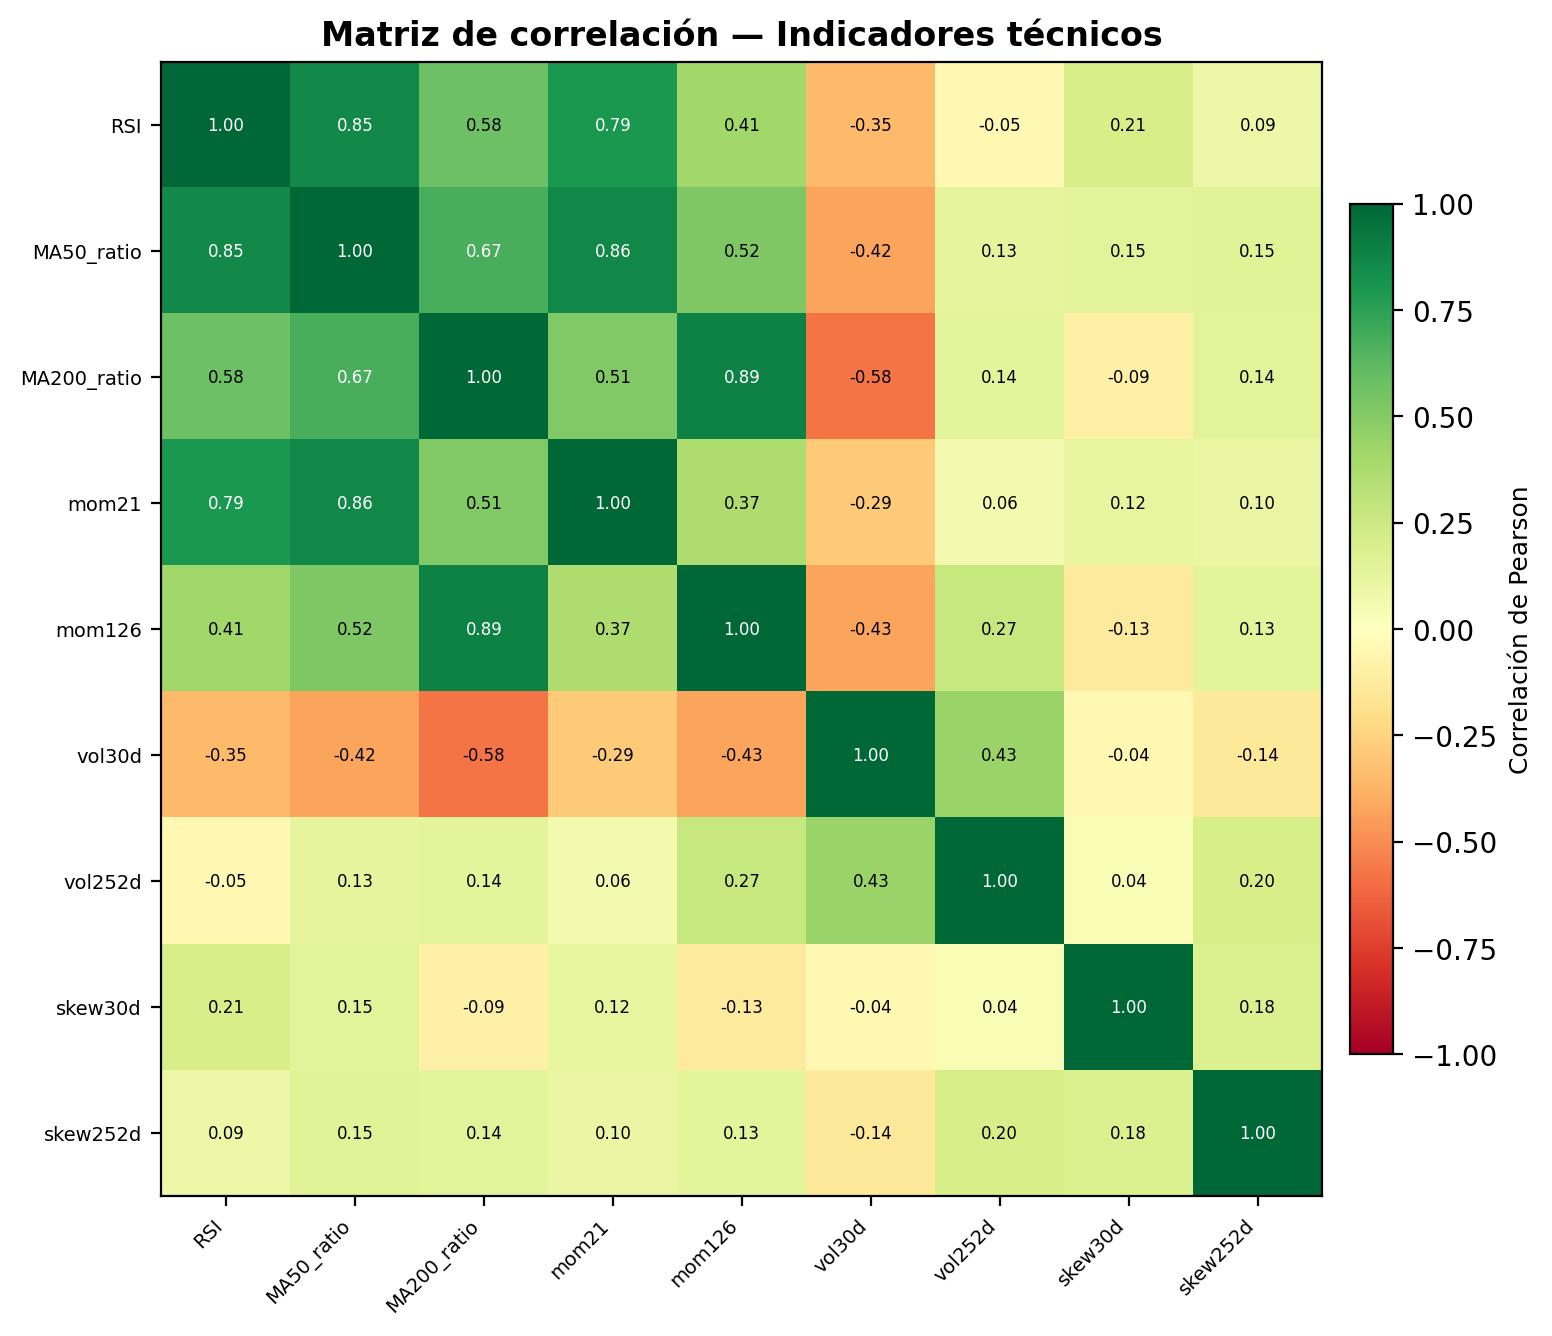
\includegraphics[width=0.85\textwidth]{figures/fig_correlation_modelA.png}
  \caption{Correlation matrix of the 9 technical features used in Model A.}
  \label{fig:correlation-modelA}
\end{figure}

For Model B, the correlation matrix additionally reveals the internal
structure of the 22 raw sentiment features. Two patterns are notable.
First, the \texttt{sentiment\_std\_<sector>} columns are strongly
positively correlated \emph{with each other} across sectors --- on days
with many news items across the market, sentiment dispersion tends to be
elevated simultaneously across most sectors, reflecting overall news
volume rather than sector-specific dynamics. Second, correlations between
sentiment features and technical features are generally \textbf{weak}
(typically below $|0.2|$), indicating that the sentiment signal captures
information that is largely \emph{orthogonal} to the price-derived
technical indicators --- a necessary (though not sufficient) condition for
sentiment to provide \emph{incremental} information to the clustering
model, rather than being redundant with the technical features already
present in Model A.

\begin{figure}[H]
  \centering
  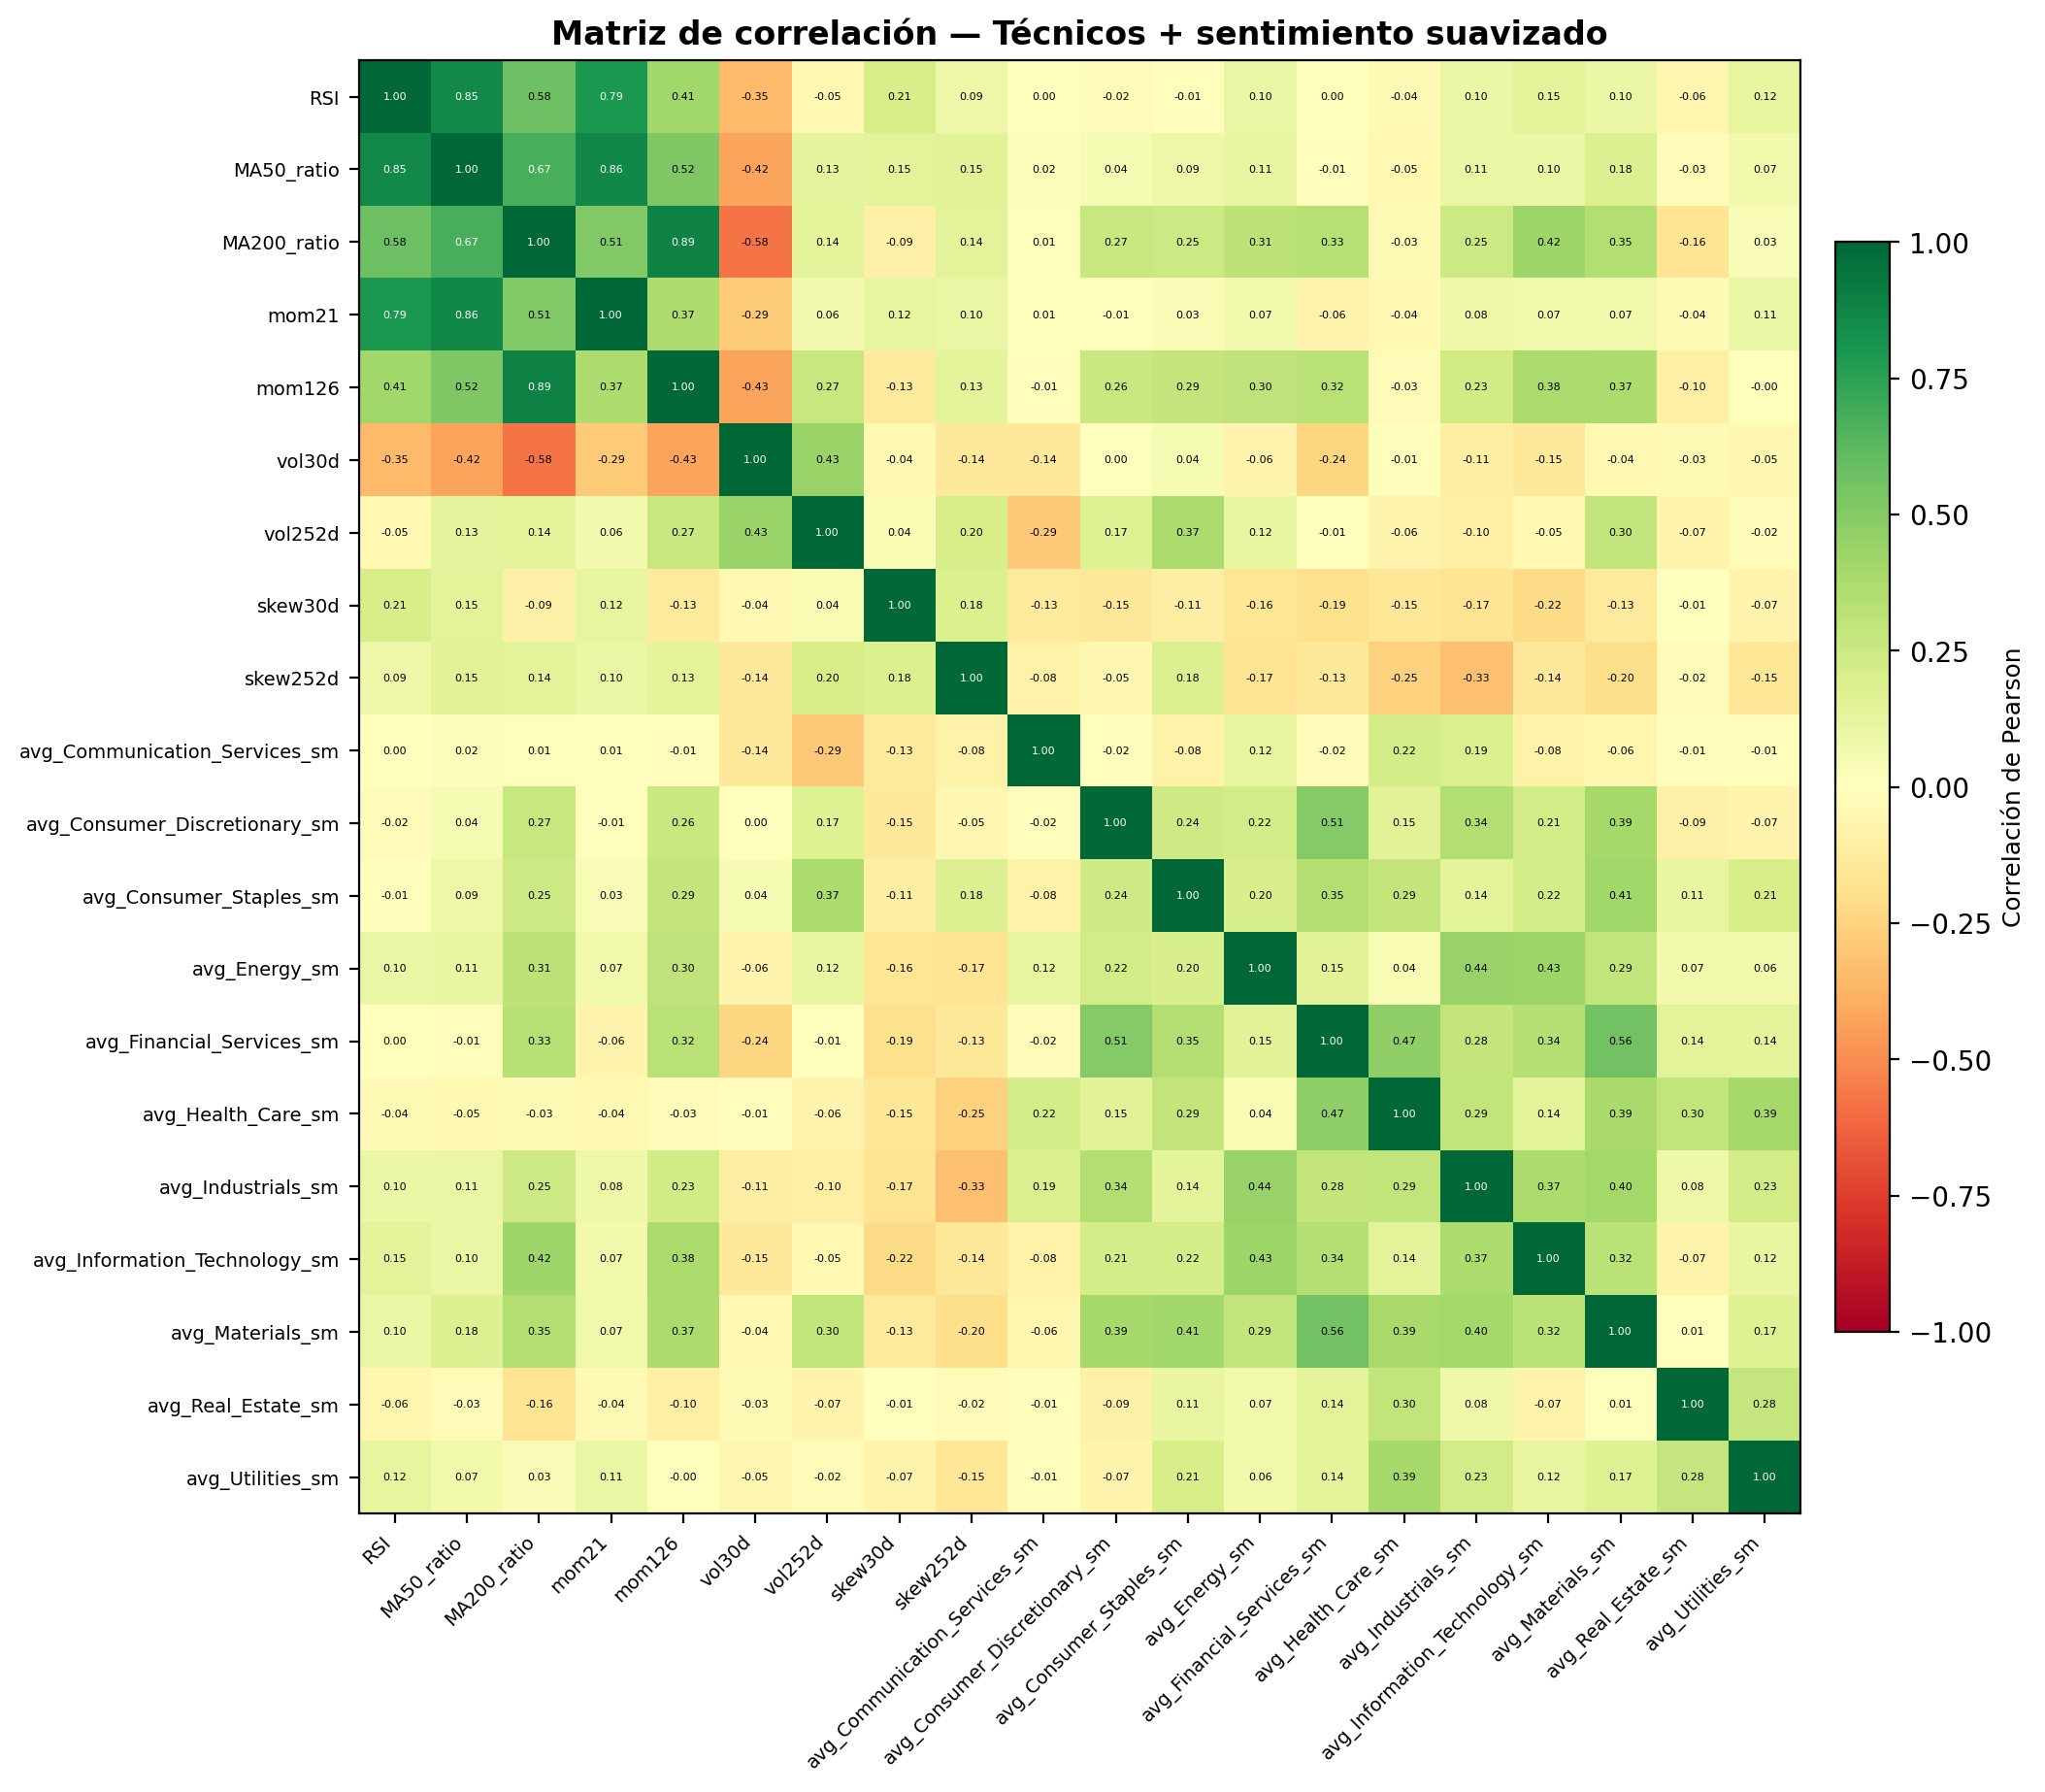
\includegraphics[width=0.95\textwidth]{figures/fig_correlation_modelB.png}
  \caption{Correlation matrix of the 31 features used in Model B (9 technical + 22 raw sector sentiment features).}
  \label{fig:correlation-modelB}
\end{figure}

\section{Feature Importance}
\label{sec:results-importance}

To assess which features contribute most to the partition produced by
Model B (\texttt{kmeans\_tech\_sent}), an ANOVA F-statistic is computed
for each feature, comparing its between-cluster variance to its
within-cluster variance: features with a large F-statistic vary
substantially \emph{across} the three regimes relative to how much they
vary \emph{within} each regime, and are therefore the features that most
strongly characterize the partition. \Cref{tab:feature-importance} reports
the top 10 features by F-statistic, and \Cref{fig:feature-importance}
shows the corresponding figure.

\begin{table}[H]
\centering
\caption{Top 10 features by ANOVA F-statistic for Model B (\texttt{kmeans\_tech\_sent}). All $p$-values are far below $10^{-50}$.}
\label{tab:feature-importance}
\small
\begin{tabular}{lllr}
\toprule
\textbf{Rank} & \textbf{Feature} & \textbf{Type} & \textbf{F-statistic} \\
\midrule
1  & MA50\_ratio\_sp500                    & Technical            & 597.81 \\
2  & RSI\_sp500                             & Technical            & 561.49 \\
3  & MA200\_ratio\_sp500                    & Technical            & 526.13 \\
4  & vol252d\_sp500                         & Technical            & 454.17 \\
5  & mom21\_sp500                           & Technical            & 366.92 \\
6  & mom126\_sp500                          & Technical            & 333.83 \\
7  & sentiment\_std\_Information Technology & Raw sentiment        & 307.21 \\
8  & sentiment\_std\_Consumer Staples       & Raw sentiment        & 295.60 \\
9  & sentiment\_std\_Consumer Discretionary & Raw sentiment        & 276.30 \\
10 & sentiment\_std\_Energy                 & Raw sentiment        & 267.58 \\
\bottomrule
\end{tabular}
\end{table}

\begin{figure}[H]
  \centering
  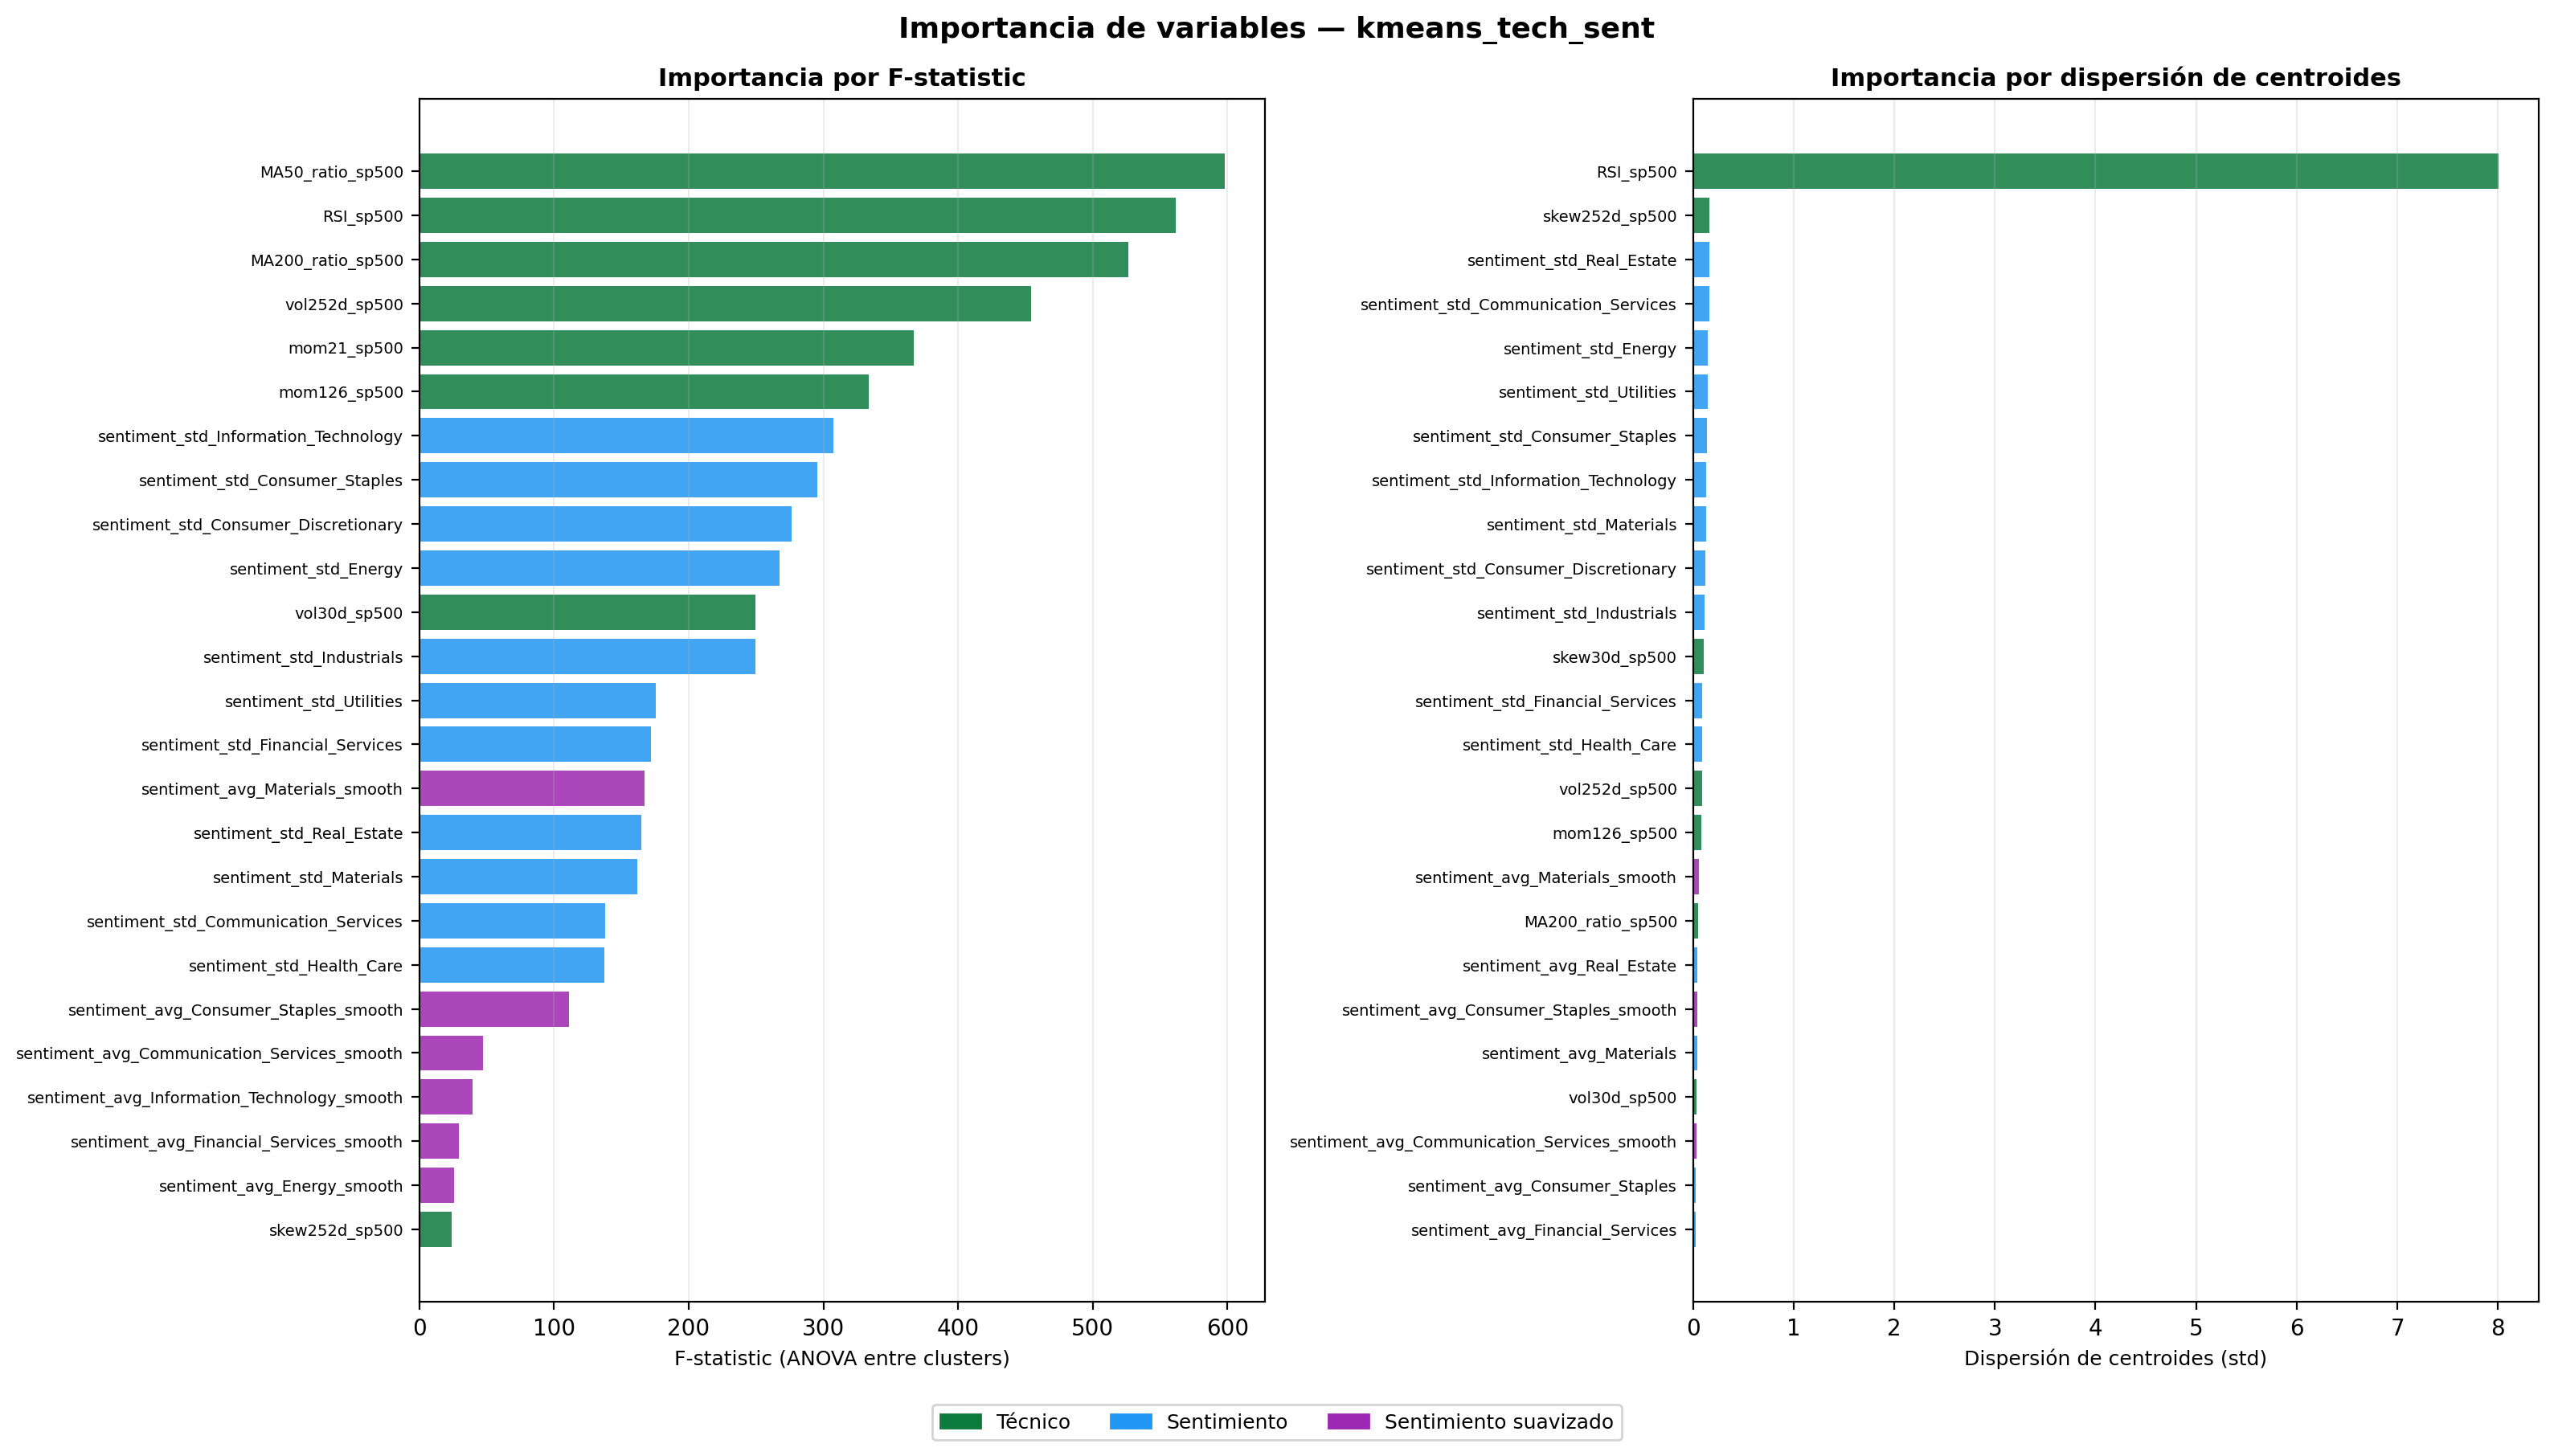
\includegraphics[width=0.95\textwidth]{figures/fig_feature_importance.png}
  \caption{ANOVA F-statistic by feature for Model B (\texttt{kmeans\_tech\_sent}), highlighting the dominance of technical features (RSI, moving-average ratios, volatility, momentum) but also the substantial contribution of sentiment-dispersion (\texttt{sentiment\_std}) features for several sectors.}
  \label{fig:feature-importance}
\end{figure}

The results in \Cref{tab:feature-importance} confirm the dominant role of
\emph{technical} features --- the top 6 features by F-statistic are all
technical indicators, with \texttt{MA50\_ratio\_sp500} ($F=597.81$) and
\texttt{RSI\_sp500} ($F=561.49$) leading. However, the \textbf{7th to
10th-ranked} features are all \texttt{sentiment\_std\_<sector>} columns
(\emph{Information Technology}, \emph{Consumer Staples}, \emph{Consumer
Discretionary} and \emph{Energy}), with F-statistics in the range
267--307 --- the same order of magnitude as \texttt{vol30d\_sp500}
($F=249.61$, ranked 11th). This indicates that the \emph{dispersion} of
sector sentiment (i.e., the degree of disagreement among simultaneous news
items about a sector) is, in fact, one of the more discriminative
sentiment-derived features for the Model B partition --- considerably more
so than the corresponding \texttt{sentiment\_avg\_<sector>} mean-sentiment
columns, all of which rank below position 20 (with F-statistics below 50).
This suggests that \emph{how much disagreement} there is in the news flow
about a sector is more informative for regime discrimination than the
\emph{average tone} of that news flow.

\section{Regime Distribution and Temporal Analysis}
\label{sec:results-regimes}

\Cref{fig:sp500-regimes-modelA} and \Cref{fig:sp500-regimes-modelB} plot
the S\&P 500 closing price over the full sample period, with the
background shaded according to the regime detected by Models A and B,
respectively (green = Bull, red = Bear, orange = Crisis). Both models
identify the \emph{Crisis} regime ($n=70$ days in both cases, 6.2\% of the
sample) almost exclusively around two episodes: the recovery phase
following the 2008--2009 financial crisis (2009) and the COVID-19 market
crash and rebound of early-to-mid 2020 --- both periods characterized by
the combination of extreme realized volatility and strong 126-session
momentum (a sharp V-shaped recovery) that defines the \emph{Crisis}
centroid in \Cref{tab:centroids-modelA,tab:centroids-modelB}.

\begin{figure}[H]
  \centering
  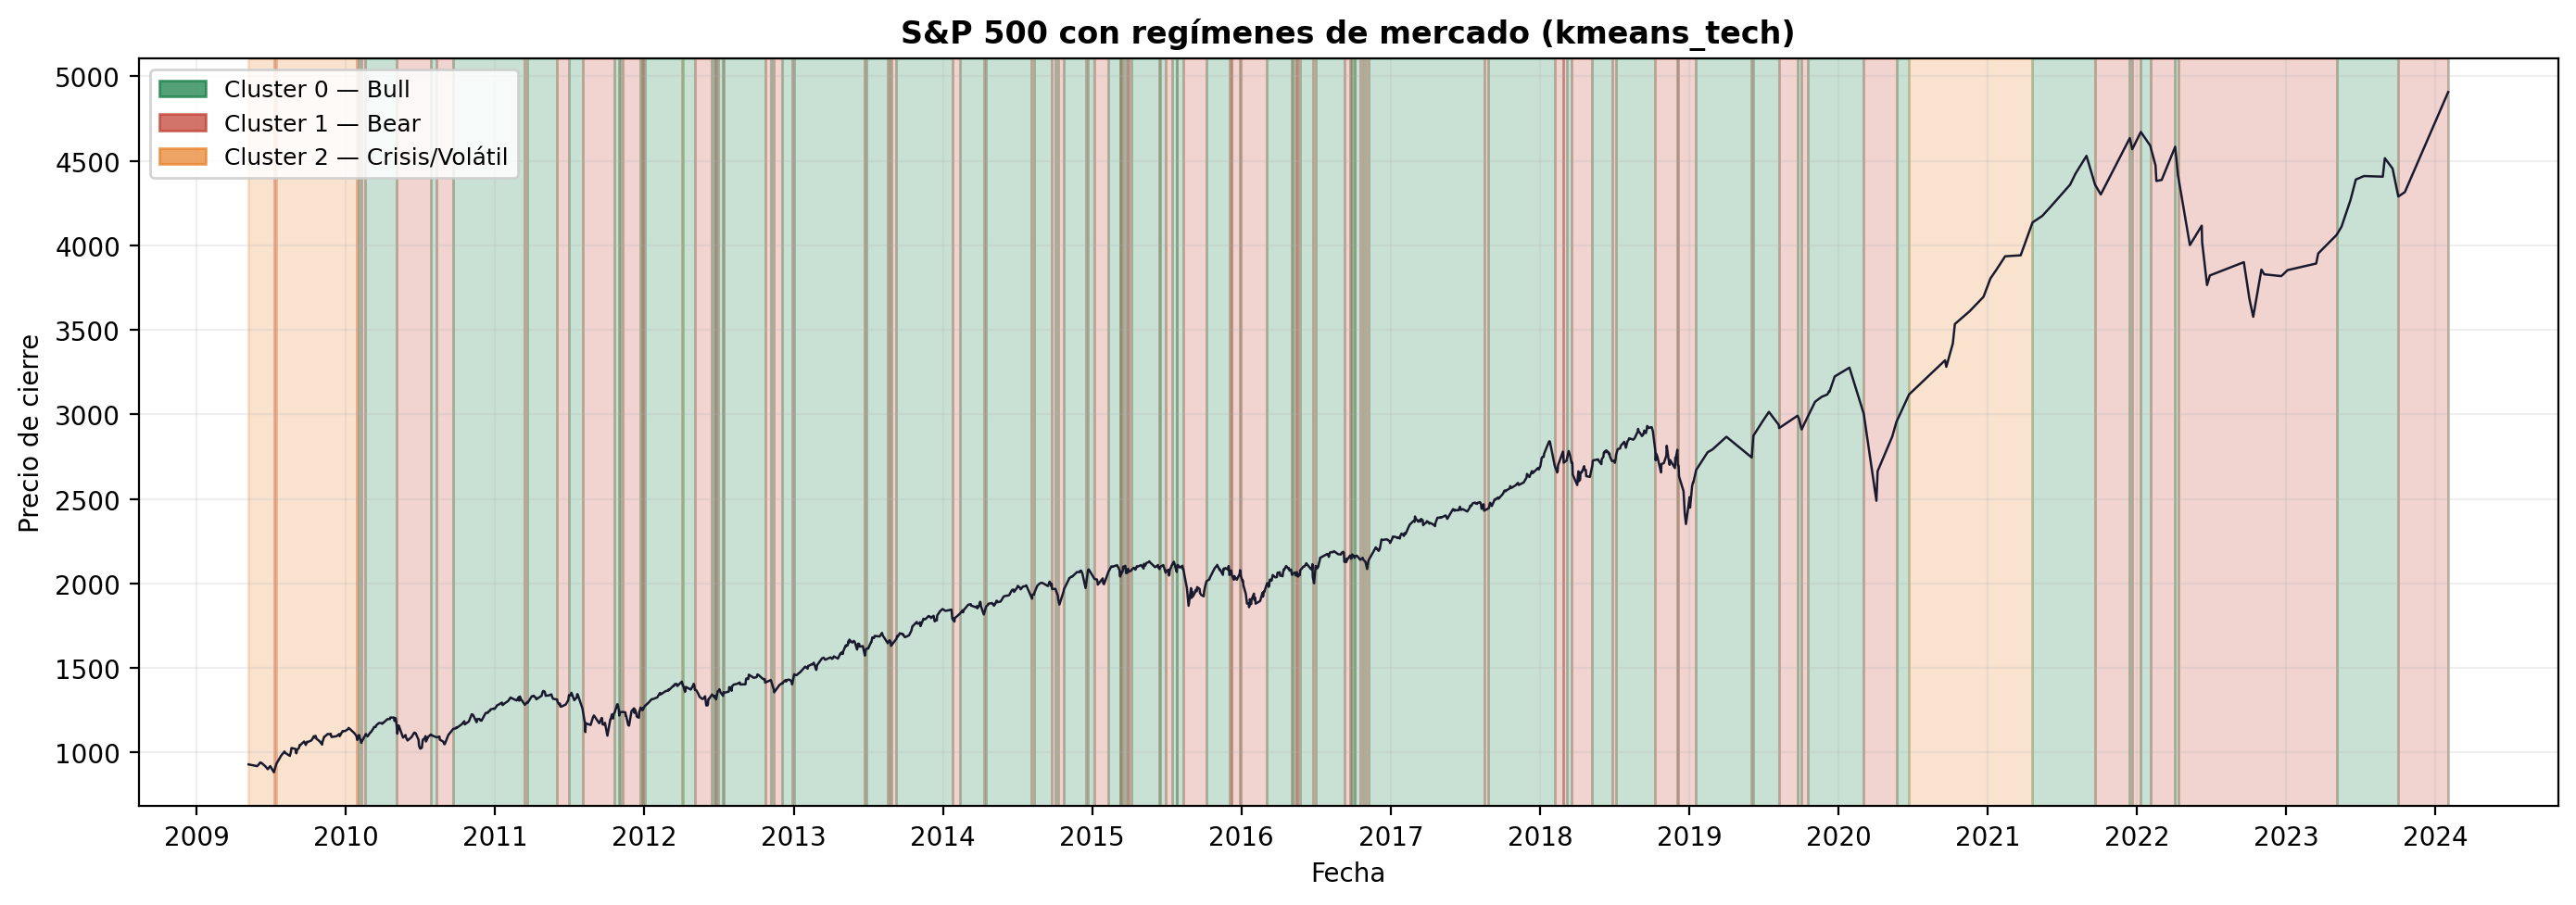
\includegraphics[width=\textwidth]{figures/fig_sp500_regimes_modelA.png}
  \caption{S\&P 500 closing price with background shading by Model A regime (\texttt{kmeans\_tech}): green = Bull, red = Bear, orange = Crisis.}
  \label{fig:sp500-regimes-modelA}
\end{figure}

\begin{figure}[H]
  \centering
  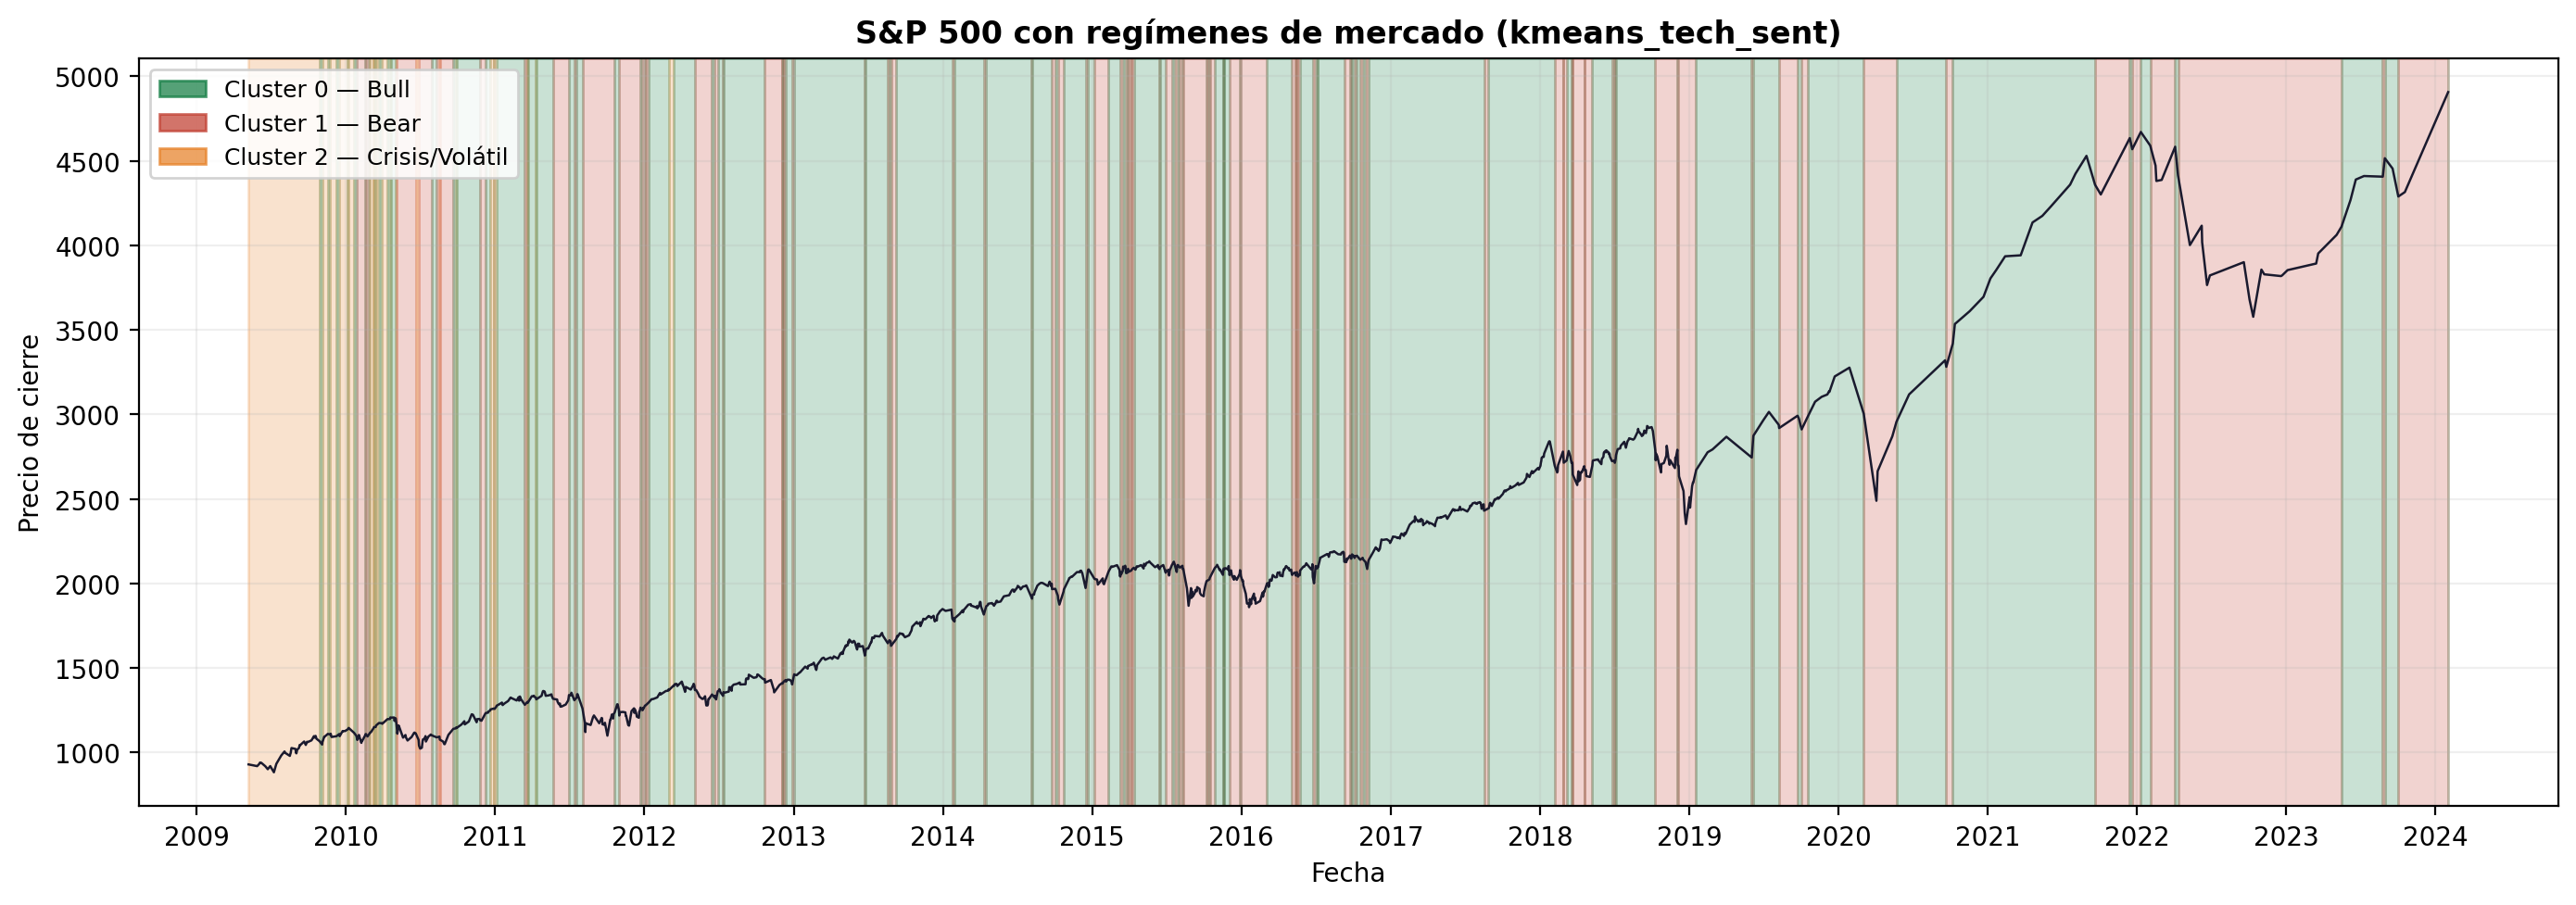
\includegraphics[width=\textwidth]{figures/fig_sp500_regimes_modelB.png}
  \caption{S\&P 500 closing price with background shading by Model B regime (\texttt{kmeans\_tech\_sent}): green = Bull, red = Bear, orange = Crisis.}
  \label{fig:sp500-regimes-modelB}
\end{figure}

The \emph{Bear} regime ($n=317$ for Model A, 28.0\%; $n=342$ for Model B,
30.2\%) is distributed across several multi-month episodes throughout the
sample, including parts of 2011 (European sovereign debt crisis), late
2015--early 2016, late 2018, and 2022. The \emph{Bull} regime is, in both
models, the majority class (65.8\% for Model A, 63.6\% for Model B),
reflecting the fact that the S\&P 500 spent the majority of the 2009--2024
sample in a long secular uptrend. The slightly larger \emph{Bear} share
and slightly smaller \emph{Bull} share in Model B relative to Model A
(and the corresponding 25-day reclassification of observations between the
two regimes, comparing $745\to720$ for Bull and $317\to342$ for Bear, with
\emph{Crisis} unchanged at $70$) indicates that incorporating sentiment
information causes a modest number of days that Model A classifies as
\emph{Bull} to be reclassified as \emph{Bear} by Model B --- consistent
with sentiment information being able to flag emerging weakness slightly
earlier or more persistently than technical indicators alone.

\Cref{fig:hmm-states-modelA} and \Cref{fig:hmm-states-modelB} show the
analogous state sequences produced by the Gaussian HMM (plotted as
\texttt{vol30d\_sp500} colored by HMM state over time, as produced by the
pipeline), which are discussed jointly with the economic comparison in
\Cref{sec:results-hmm}.

\begin{figure}[H]
  \centering
  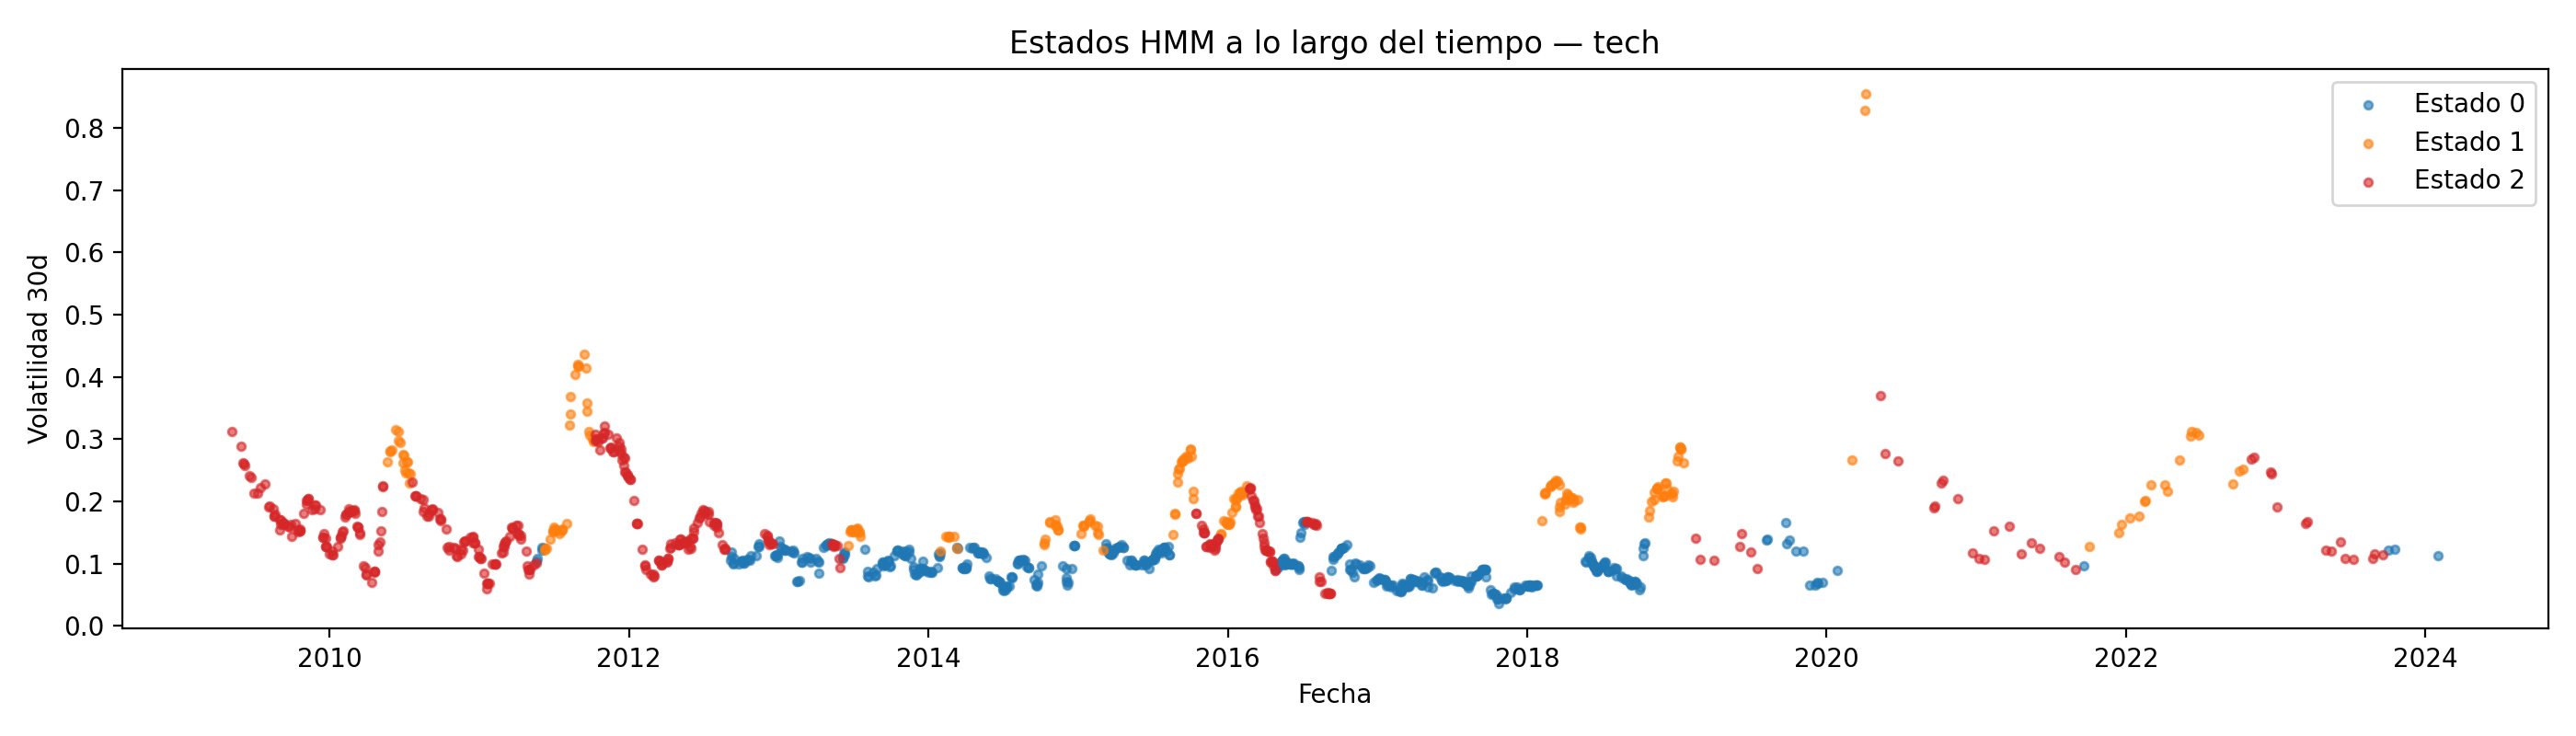
\includegraphics[width=\textwidth]{figures/fig_hmm_states_modelA.png}
  \caption{30-day realized volatility of the S\&P 500 over time, colored by Gaussian HMM state (\texttt{hmm\_tech}, fitted on the 9 technical features).}
  \label{fig:hmm-states-modelA}
\end{figure}

\begin{figure}[H]
  \centering
  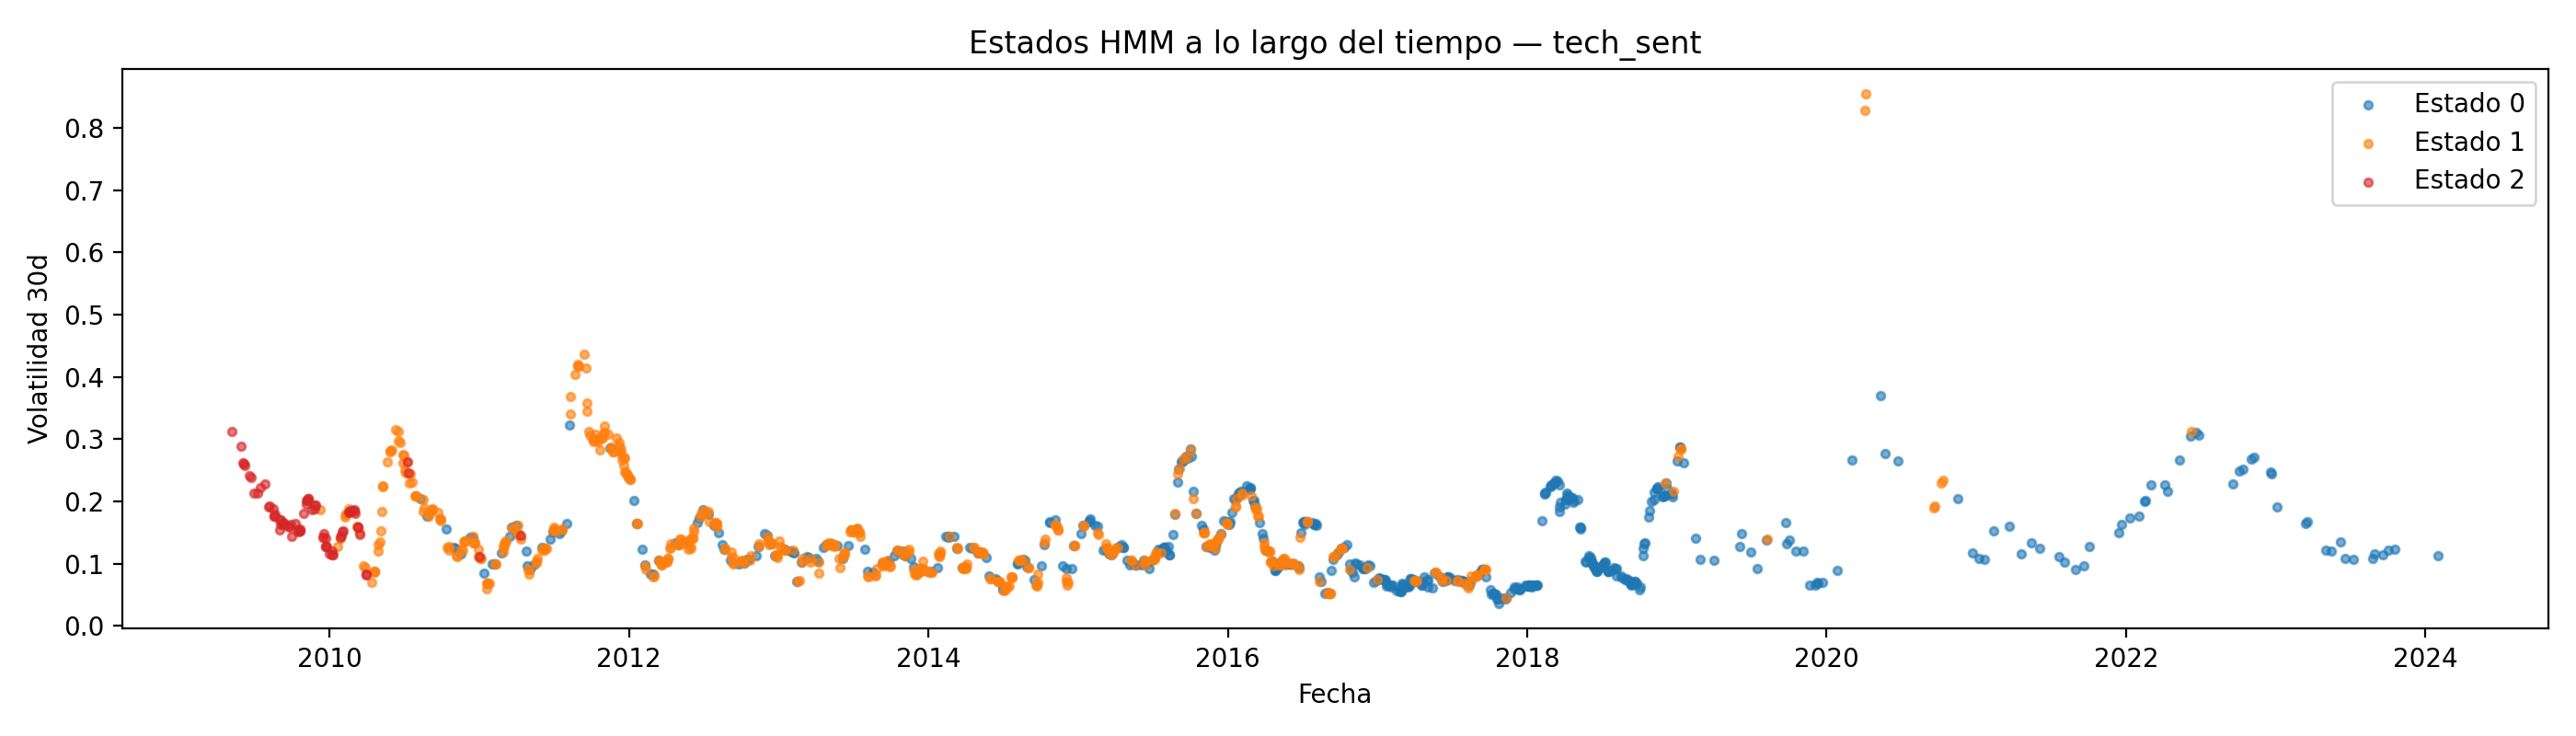
\includegraphics[width=\textwidth]{figures/fig_hmm_states_modelB.png}
  \caption{30-day realized volatility of the S\&P 500 over time, colored by Gaussian HMM state (\texttt{hmm\_tech\_sent}, fitted on the 31 technical + raw sentiment features).}
  \label{fig:hmm-states-modelB}
\end{figure}

\Cref{fig:sp500-regimes-hmm} shows the same regime-shading representation
as \Cref{fig:sp500-regimes-modelA,fig:sp500-regimes-modelB}, but for the
\texttt{hmm\_tech\_sent} state sequence. Visually, the HMM's \emph{Bear}
state (red) occupies a substantially larger fraction of the timeline than
the \textit{K-Means} \emph{Bear} regime, including extended stretches of
2011--2012, 2015--2016, 2018, 2020 and 2022 that \textit{K-Means} instead
assigns predominantly to \emph{Bull}. This is consistent with the
narrower, less extreme Sharpe ratios reported for the HMM in
\Cref{tab:market-hmm}: a \emph{Bear} state that includes a much larger and
more heterogeneous set of days necessarily has a less negative average
return than a \emph{Bear} regime restricted to the sharpest downturns.

\begin{figure}[H]
  \centering
  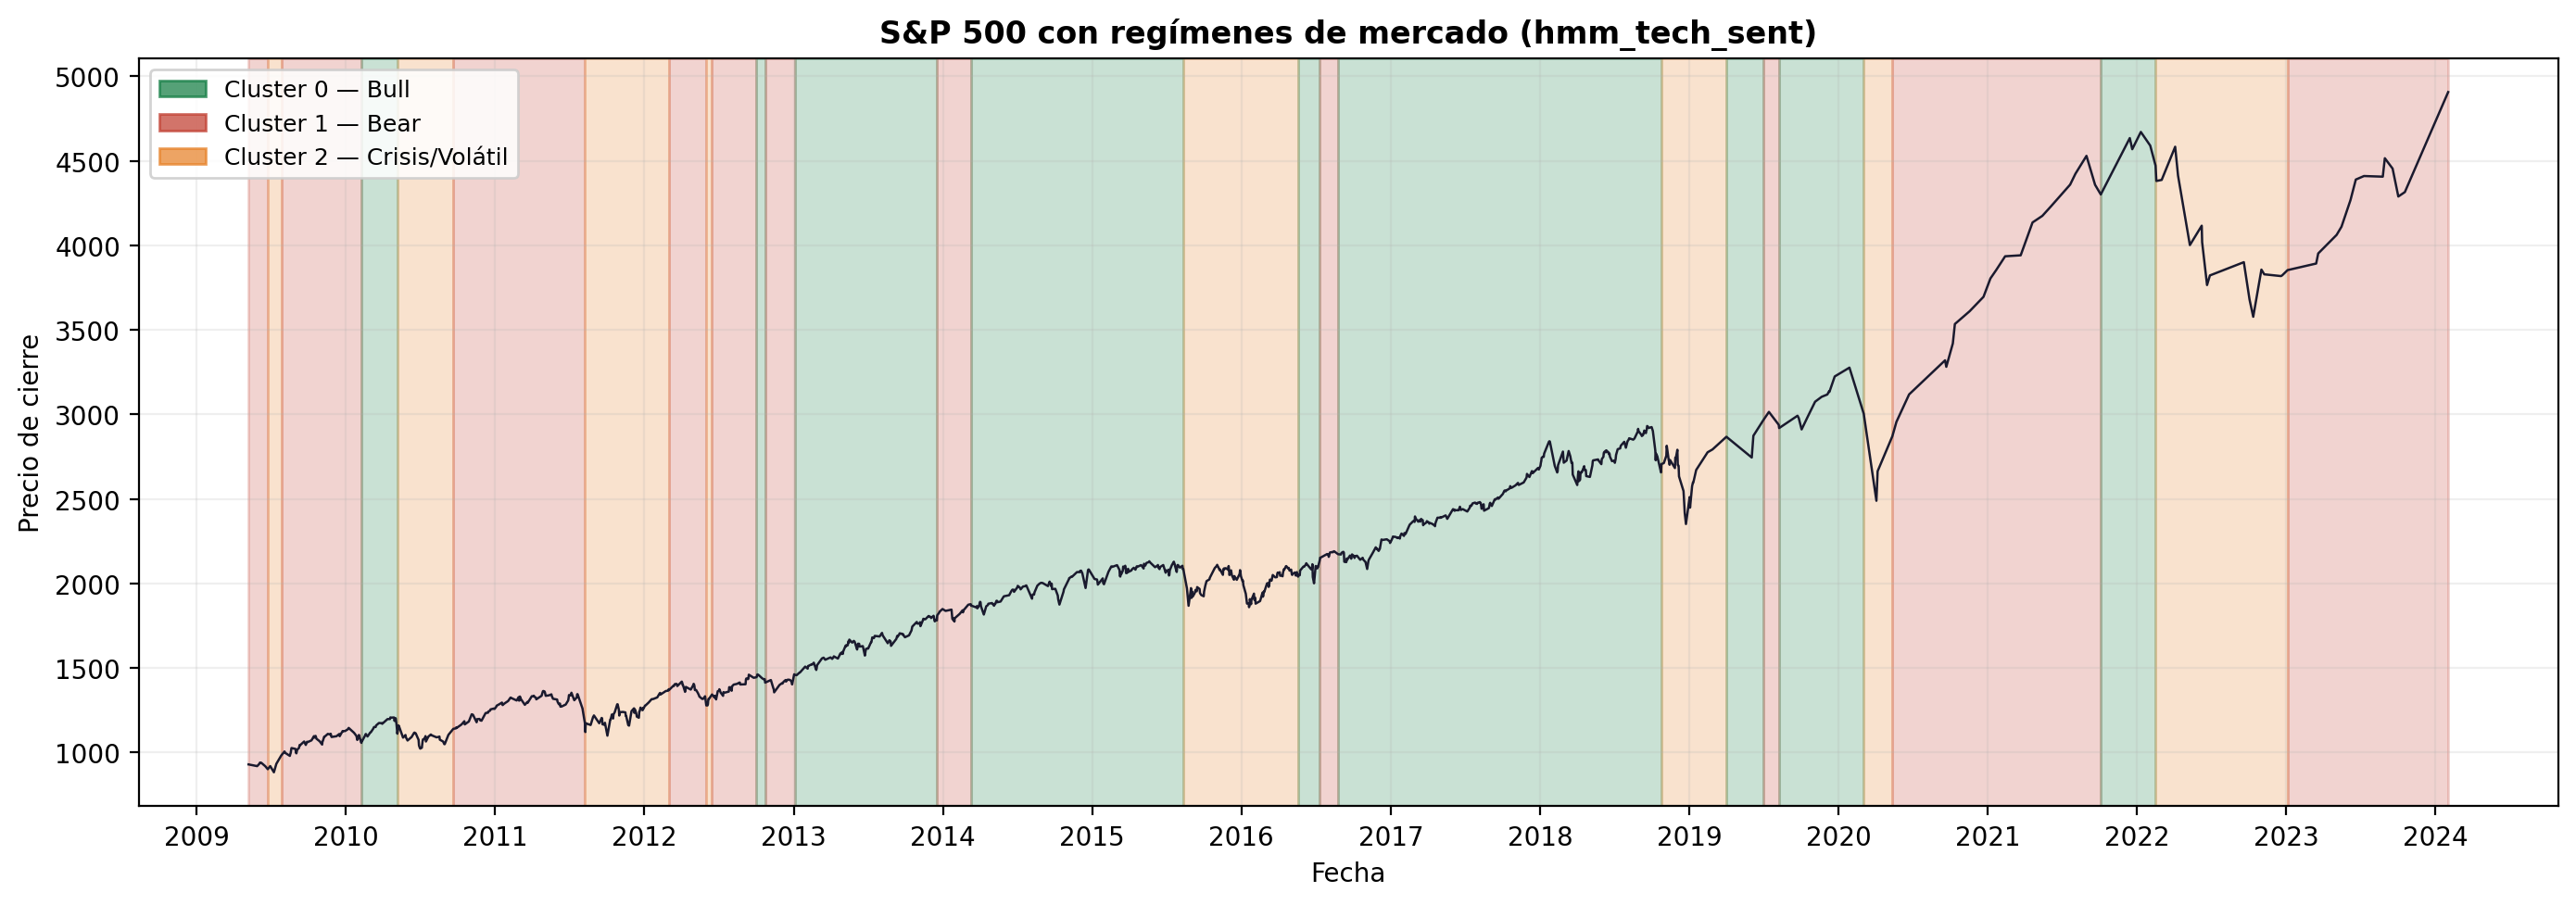
\includegraphics[width=\textwidth]{figures/fig_sp500_regimes_hmm.png}
  \caption{S\&P 500 closing price with background shading by Gaussian HMM state (\texttt{hmm\_tech\_sent}): green = Bull, red = Bear, orange = Crisis/Volatile.}
  \label{fig:sp500-regimes-hmm}
\end{figure}

\section{Economic Validation: Overall Market-Level Metrics}
\label{sec:results-econ-overall}

Before turning to the sector-level breakdown, this section reports the
economic profile of each regime computed directly on the \emph{aggregate}
S\&P 500 daily returns (i.e., not yet broken down by GICS sector), for all
five clustering configurations: Models A, B, C (\textit{K-Means}) and the
two HMM variants (\texttt{hmm\_tech}, \texttt{hmm\_tech\_sent}).
\Cref{tab:market-kmeans} and \Cref{tab:market-hmm} report, for each
regime/state, the number of days, the mean daily return, the annualized
volatility, the Sharpe ratio, the percentage of positive days, and the
best/worst single-day returns.

\begin{table}[H]
\centering
\caption{Market-level (S\&P 500) economic profile by regime, K-Means Models A, B and C. $n=1{,}132$ observations per model.}
\label{tab:market-kmeans}
\small
\begin{tabular}{llrrrrrr}
\toprule
\textbf{Model} & \textbf{Regime} & \textbf{$n$} & \textbf{Mean daily ret.\ (\%)} & \textbf{Ann.\ vol.} & \textbf{Sharpe} & \textbf{\% pos.\ days} & \textbf{Worst / Best day (\%)} \\
\midrule
A & Bull    & 745 & 0.1565  & 0.1018 & 3.68  & 59.7 & $-2.50$ / $3.37$ \\
A & Bear    & 317 & $-$0.2830 & 0.2352 & $-3.12$ & 41.6 & $-4.52$ / $6.80$ \\
A & Crisis  & 70  & 0.2315  & 0.1720 & 3.28  & 60.0 & $-2.46$ / $2.92$ \\
\midrule
B & Bull    & 720 & 0.1650  & 0.1035 & 3.82  & 60.0 & $-2.50$ / $3.37$ \\
B & Bear    & 342 & $-$0.2700 & 0.2289 & $-3.06$ & 42.1 & $-4.52$ / $6.80$ \\
B & Crisis  & 70  & 0.2369  & 0.1537 & 3.75  & 61.4 & $-2.46$ / $2.92$ \\
\midrule
C & Bull    & 534 & 0.0643  & 0.1711 & 0.83  & 53.9 & $-4.52$ / $4.63$ \\
C & Bear    & 172 & 0.1012  & 0.1386 & 1.70  & 58.7 & $-2.11$ / $2.92$ \\
C & Crisis  & 426 & $-$0.0204 & 0.1490 & $-0.48$ & 54.0 & $-3.34$ / $6.80$ \\
\bottomrule
\end{tabular}
\end{table}

\begin{table}[H]
\centering
\caption{Market-level (S\&P 500) economic profile by state, Gaussian HMM fitted on Model A and Model B feature sets. $n=1{,}132$ observations per model.}
\label{tab:market-hmm}
\small
\begin{tabular}{llrrrrrr}
\toprule
\textbf{HMM} & \textbf{State} & \textbf{$n$} & \textbf{Mean daily ret.\ (\%)} & \textbf{Ann.\ vol.} & \textbf{Sharpe} & \textbf{\% pos.\ days} & \textbf{Worst / Best day (\%)} \\
\midrule
\texttt{hmm\_tech}      & 0 & 514 & 0.0239  & 0.1091 & 0.37  & 53.7 & $-3.66$ / $2.51$ \\
\texttt{hmm\_tech}      & 1 & 213 & $-$0.0523 & 0.2406 & $-0.63$ & 54.0 & $-4.52$ / $6.80$ \\
\texttt{hmm\_tech}      & 2 & 405 & 0.1035  & 0.1567 & 1.54  & 56.3 & $-2.86$ / $4.30$ \\
\midrule
\texttt{hmm\_tech\_sent} & 0 & 575 & 0.0418  & 0.1117 & 0.76  & 55.5 & $-3.66$ / $2.20$ \\
\texttt{hmm\_tech\_sent} & 1 & 293 & 0.0789  & 0.1434 & 1.25  & 54.3 & $-2.46$ / $2.51$ \\
\texttt{hmm\_tech\_sent} & 2 & 264 & $-$0.0155 & 0.2403 & $-0.25$ & 53.4 & $-4.52$ / $6.80$ \\
\bottomrule
\end{tabular}
\end{table}

Two important results emerge from \Cref{tab:market-kmeans}. First, for
Models A and B, the \textbf{Bear} regime is the only one with a
\emph{negative} Sharpe ratio ($-3.12$ for A, $-3.06$ for B), confirming
that the labeling heuristic of \Cref{sec:meth-labeling} correctly
identifies the regime associated with negative aggregate market
performance. Second, both the \textbf{Bull} and \textbf{Crisis} regimes
have \emph{positive} Sharpe ratios at the aggregate market level (around
$+3.3$ to $+3.8$) --- the \emph{Crisis} regime is not, in aggregate, a
period of negative returns, but rather a period of \emph{both} elevated
volatility \emph{and} elevated mean returns, consistent with its
identification with the sharp V-shaped recoveries of 2009 and 2020.
Comparing Model A and B's Sharpe ratios for each regime shows that Model B
produces a (slightly) \emph{more extreme} Bull Sharpe ($3.82$ vs.\ $3.68$)
and a (slightly) \emph{less extreme} Bear Sharpe ($-3.06$ vs.\ $-3.12$),
alongside a higher Crisis Sharpe ($3.75$ vs.\ $3.28$); the net effect of
incorporating sentiment is therefore a moderate \emph{sharpening} of the
Bull/Crisis vs.\ Bear contrast at the aggregate level.

\Cref{tab:market-hmm} is discussed in detail in \Cref{sec:results-hmm}, but
the key observation is immediately visible: the Sharpe ratios for the HMM
states range only from $-0.63$ to $+1.54$, a far narrower range than the
$-3.12$ to $+3.82$ range observed for the \textit{K-Means} models.

\section{Economic Validation: Sector-Level Heatmaps}
\label{sec:results-econ-sector}

This section presents the sector-level economic validation results,
obtained by reindexing each model's regime labels onto the daily sector
return series (\Cref{sec:meth-validation}) and computing, for each of the
11 GICS sectors and 3 regimes, the metrics of
\Cref{eq:ann-return}--\Cref{eq:max-dd}. After reindexing, each model labels
$3{,}695$ sector-days, distributed as follows: Model A --- Bull 2{,}108
(57.0\%), Bear 1{,}214 (32.9\%), Crisis 373 (10.1\%); Model B --- Bull
2{,}196 (59.4\%), Bear 1{,}301 (35.2\%), Crisis 198 (5.4\%); Model C ---
Bull 1{,}571 (42.5\%), Bear 436 (11.8\%), Crisis 1{,}688 (45.7\%). Complete
per-sector tables for all three models are provided in Annex~B
(\Cref{tab:annexB-modelA,tab:annexB-modelB,tab:annexB-modelC}); this
section focuses on the headline patterns, illustrated through the Sharpe
ratio, maximum drawdown, and best/worst single-day return heatmaps for
Model B (the technical+sentiment model, which is the primary object of
comparison in this thesis).

\begin{figure}[H]
  \centering
  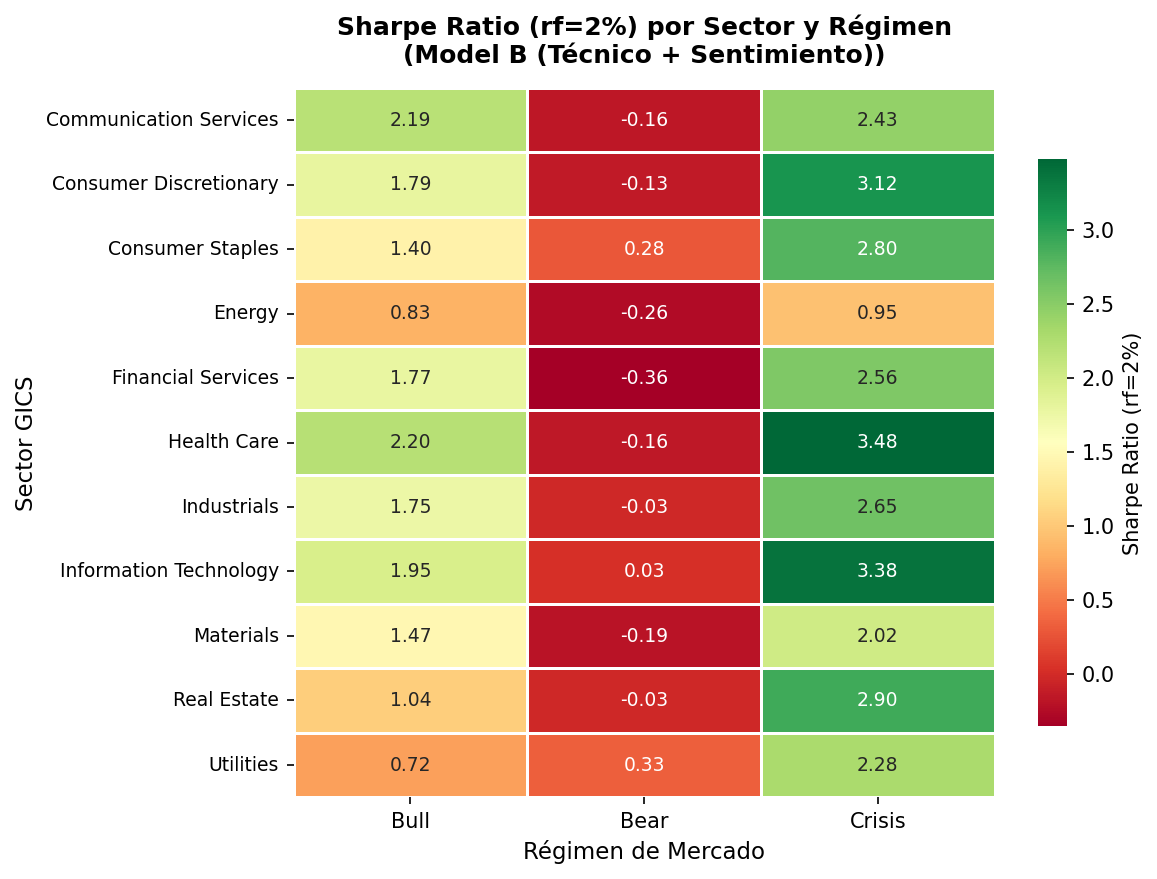
\includegraphics[width=0.85\textwidth]{figures/fig_heatmap_sharpe_modelB.png}
  \caption{Sharpe ratio by GICS sector and regime, Model B (\texttt{kmeans\_tech\_sent}).}
  \label{fig:heatmap-sharpe-modelB}
\end{figure}

\Cref{fig:heatmap-sharpe-modelB} shows that the \textbf{Bear} regime
produces a \emph{negative} Sharpe ratio for \textbf{10 of the 11 GICS
sectors} (all except \emph{Consumer Staples}, which remains marginally
positive at $0.28$), with the most negative values observed in
\emph{Financial Services} ($-0.36$), \emph{Energy} ($-0.26$),
\emph{Materials} ($-0.19$) and \emph{Real Estate} ($-0.19$). This is the
clearest evidence that the \emph{Bear} regime, as detected by Model B,
corresponds to a genuinely adverse environment across virtually the entire
equity market, not merely for the aggregate index. By contrast, the
\textbf{Crisis} regime shows the \emph{highest} Sharpe ratio for every
single sector, ranging from $0.95$ (\emph{Energy}) to as high as $3.48$
(\emph{Health Care}) and $3.38$ (\emph{Information Technology}). Averaged
across sectors, the mean regime Sharpe ratios for Model B are $1.56$
(Bull), $-0.06$ (Bear) and $2.60$ (Crisis) --- the same qualitative pattern
observed at the aggregate market level in \Cref{tab:market-kmeans}, now
confirmed to hold sector-by-sector.

\begin{figure}[H]
  \centering
  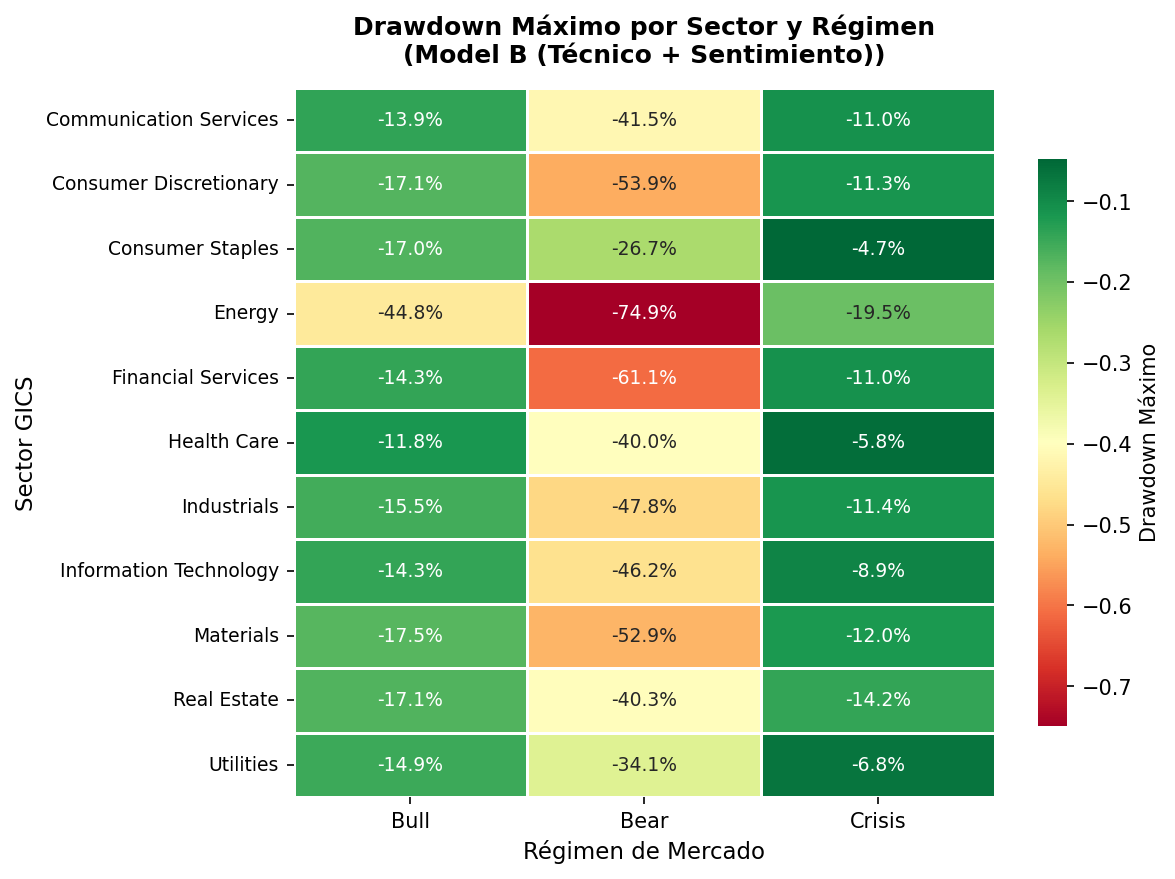
\includegraphics[width=0.85\textwidth]{figures/fig_heatmap_maxdd_modelB.png}
  \caption{Maximum (within-regime) drawdown by GICS sector and regime, Model B (\texttt{kmeans\_tech\_sent}).}
  \label{fig:heatmap-maxdd-modelB}
\end{figure}

\Cref{fig:heatmap-maxdd-modelB} shows that the single most severe
within-regime drawdown across the entire analysis occurs for
\textbf{\emph{Energy} in the \emph{Bear} regime}, at $-74.9\%$ --- more
than 20 percentage points worse than the next most severe combination
(\emph{Financial Services}/Bear at $-61.1\%$). Averaged across sectors,
the mean maximum drawdown by regime is $-18.0\%$ (Bull), $-47.2\%$ (Bear)
and $-10.6\%$ (Crisis): the \emph{Bear} regime is associated with
substantially deeper drawdowns than \emph{Crisis}, despite \emph{Crisis}
having higher \emph{point-in-time} volatility (\Cref{tab:centroids-modelB}).
This apparent paradox is resolved by recalling that \emph{Crisis} days are
characterized by \emph{both} large negative \emph{and} large positive
daily moves (high volatility with a strong rebound component, captured by
the elevated \texttt{mom126\_sp500} centroid), whereas \emph{Bear} days
tend to be more \emph{persistently} negative, allowing losses to compound
into deeper drawdowns even though individual daily moves are, on average,
less extreme.

\begin{figure}[H]
  \centering
  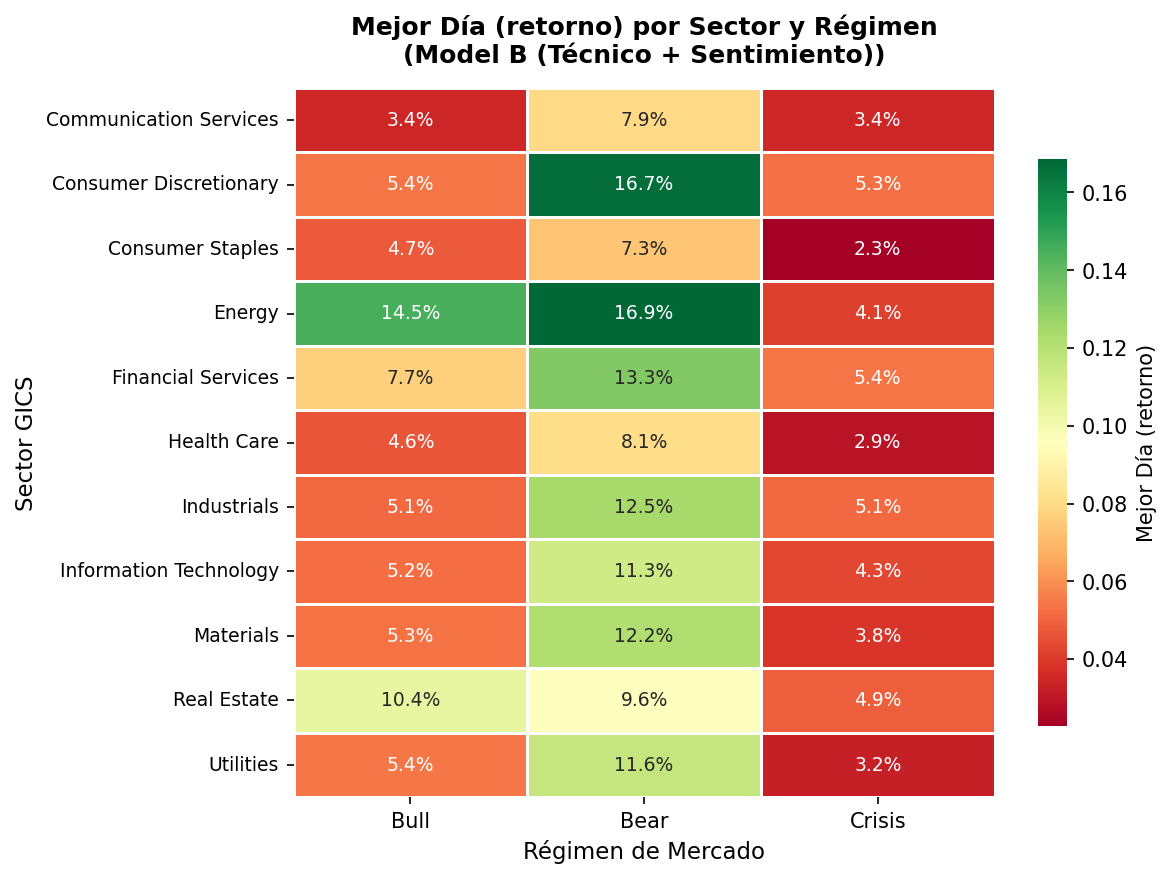
\includegraphics[width=0.85\textwidth]{figures/fig_heatmap_bestday_modelB.png}
  \caption{Best single-day return by GICS sector and regime, Model B (\texttt{kmeans\_tech\_sent}).}
  \label{fig:heatmap-bestday-modelB}
\end{figure}

\begin{figure}[H]
  \centering
  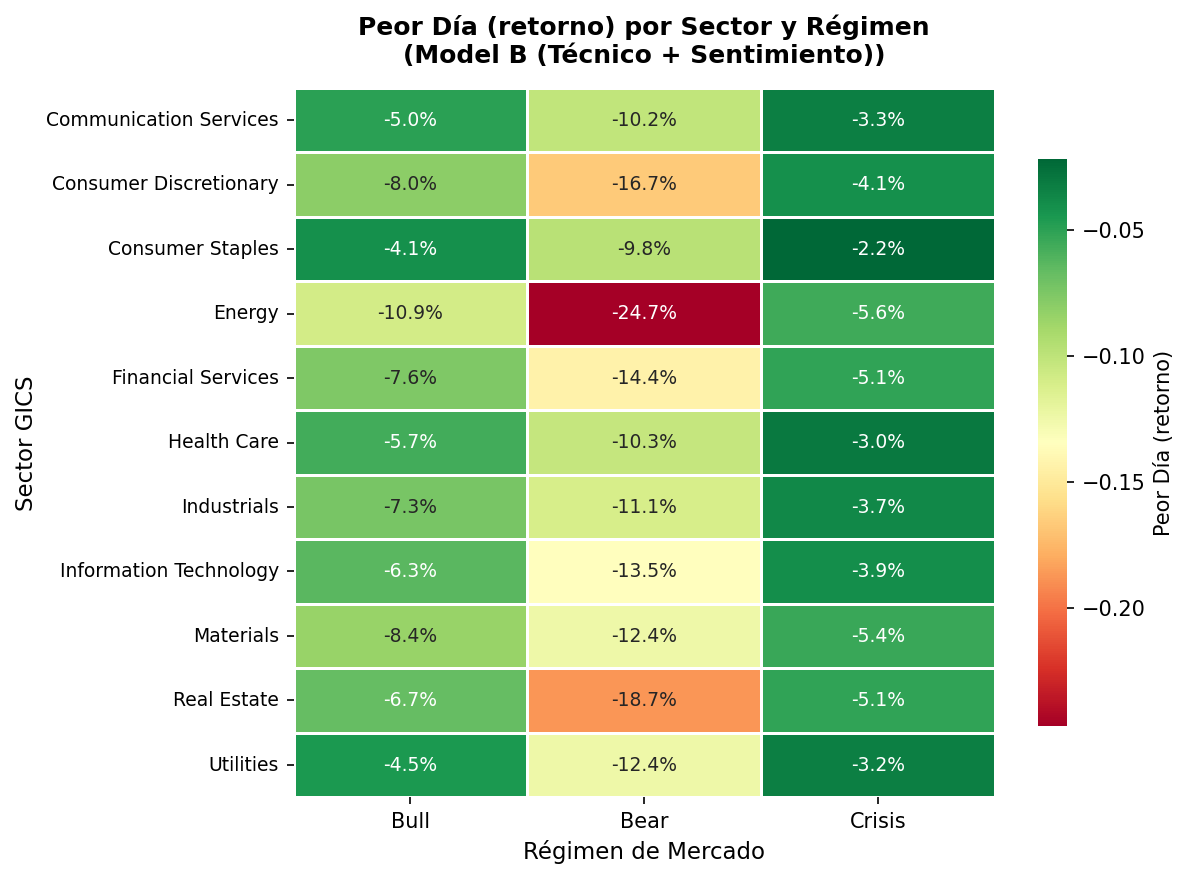
\includegraphics[width=0.85\textwidth]{figures/fig_heatmap_worstday_modelB.png}
  \caption{Worst single-day return by GICS sector and regime, Model B (\texttt{kmeans\_tech\_sent}).}
  \label{fig:heatmap-worstday-modelB}
\end{figure}

\Cref{fig:heatmap-bestday-modelB,fig:heatmap-worstday-modelB} reveal a
striking fact: the \textbf{single best day} ($+16.9\%$) \emph{and} the
\textbf{single worst day} ($-24.7\%$) of the \emph{entire dataset}, across
all sectors and all regimes, both occur for \textbf{\emph{Energy} in the
\emph{Bear} regime}. This confirms that, for Model B, the \emph{Bear}
regime --- rather than \emph{Crisis} --- is where the most extreme
single-day tail events are concentrated for the \emph{Energy} sector,
likely reflecting episodes such as the April 2020 negative oil-price
shock, which combined a severe and \emph{persistent} (Bear-like) downturn
in energy markets with extreme single-day volatility.

The corresponding Sharpe-ratio heatmaps for Models A and C are shown in
\Cref{fig:heatmap-sharpe-modelA,fig:heatmap-sharpe-modelC} for reference;
Model A shows a qualitatively similar but slightly less extreme pattern
than Model B (mean regime Sharpe ratios of $1.41$, $-0.07$ and $2.44$ for
Bull, Bear and Crisis respectively), while Model C is discussed separately
in \Cref{sec:results-modelC}.

\begin{figure}[H]
  \centering
  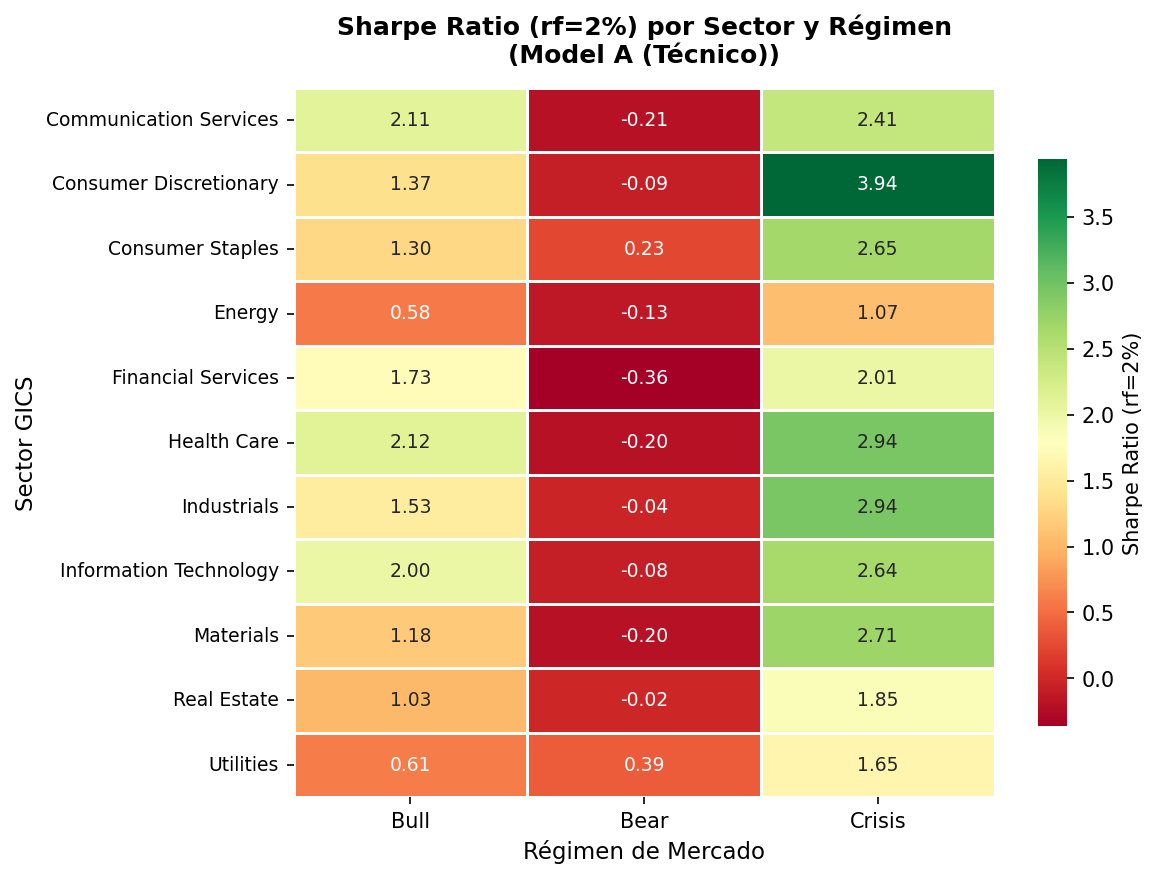
\includegraphics[width=0.85\textwidth]{figures/fig_heatmap_sharpe_modelA.png}
  \caption{Sharpe ratio by GICS sector and regime, Model A (\texttt{kmeans\_tech}).}
  \label{fig:heatmap-sharpe-modelA}
\end{figure}

\section{Model C: A Negative Result}
\label{sec:results-modelC}

Model C clusters days using \emph{exclusively} the 11 MA21-smoothed sector
sentiment features, with no technical (price-derived) information
whatsoever. \Cref{fig:heatmap-sharpe-modelC} shows the resulting Sharpe
ratio heatmap.

\begin{figure}[H]
  \centering
  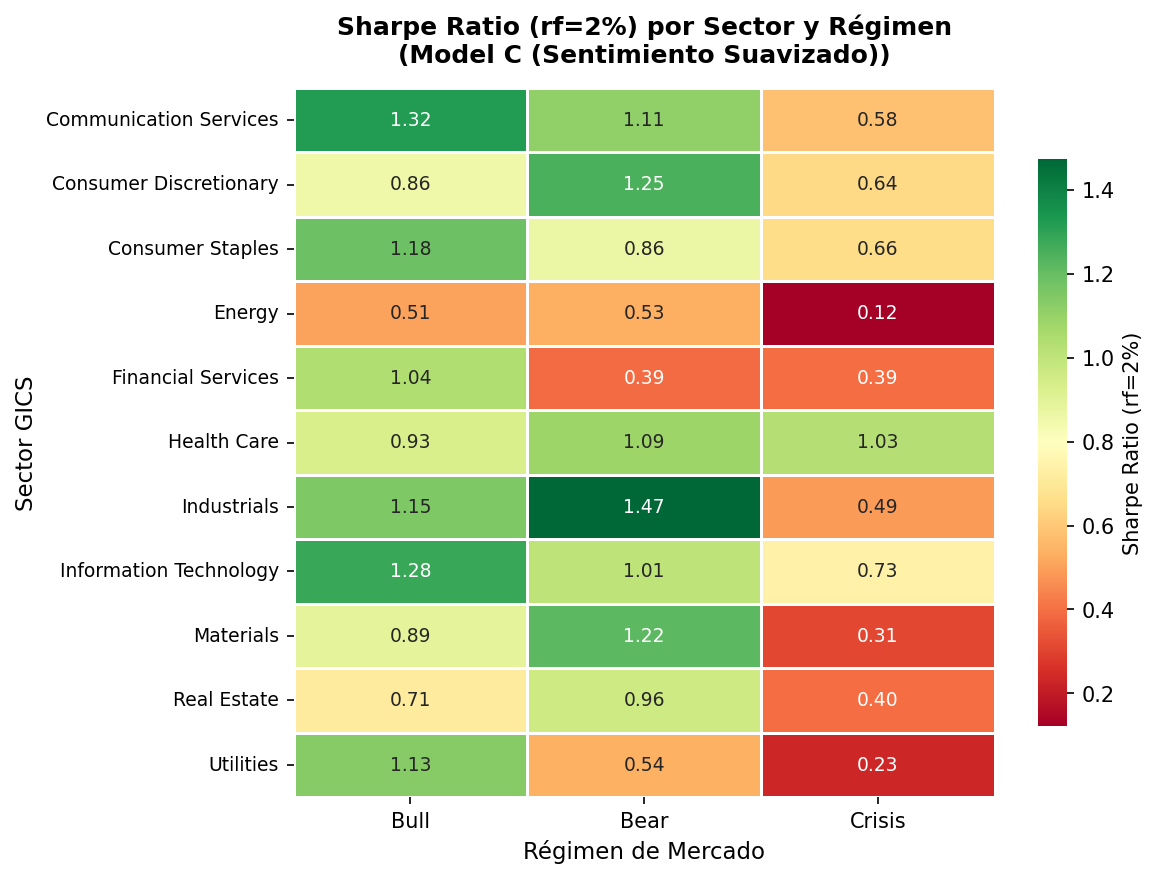
\includegraphics[width=0.85\textwidth]{figures/fig_heatmap_sharpe_modelC.png}
  \caption{Sharpe ratio by GICS sector and regime, Model C (\texttt{kmeans\_sent\_smooth}).}
  \label{fig:heatmap-sharpe-modelC}
\end{figure}

Two pieces of evidence jointly indicate that Model C fails to recover
regimes with a technical/economic profile comparable to Models A and B.

First, \textbf{the technical centroids of Model C's three clusters are
nearly indistinguishable} (\Cref{tab:centroids-modelC}). For example,
\texttt{MA50\_ratio\_sp500} ranges only from $1.0086$ to $1.0134$ across
Model C's clusters --- a spread of $0.0048$ --- compared to a spread of
$0.0653$ for Model A ($0.9739$ to $1.0392$) and $0.0608$ for Model B. The
\texttt{RSI\_sp500} centroids similarly range only from $54.4$ to $56.2$
for Model C, compared to $42.6$--$60.3$ for Model A.

\begin{table}[H]
\centering
\caption{Model C (smoothed sentiment only): centroids in the \emph{technical} feature space (for comparison with Models A and B), and cluster sizes.}
\label{tab:centroids-modelC}
\small
\begin{tabular}{lrrr}
\toprule
\textbf{Feature} & \textbf{Cluster 0} & \textbf{Cluster 1} & \textbf{Cluster 2} \\
\midrule
RSI\_sp500          & 54.86 & 54.44 & 56.18 \\
MA50\_ratio\_sp500  & 1.0086 & 1.0134 & 1.0109 \\
MA200\_ratio\_sp500 & 1.0274 & 1.0924 & 1.0496 \\
mom21\_sp500        & 0.0081 & 0.0063 & 0.0094 \\
mom126\_sp500       & 0.0379 & 0.1397 & 0.0683 \\
vol30d\_sp500       & 0.1532 & 0.1389 & 0.1260 \\
vol252d\_sp500      & 0.1633 & 0.2135 & 0.1402 \\
skew30d\_sp500      & $-$0.0460 & $-$0.3928 & $-$0.2998 \\
skew252d\_sp500     & $-$0.3193 & $-$0.3215 & $-$0.5746 \\
\midrule
\textbf{$n$ (days)}  & \textbf{534} & \textbf{172} & \textbf{426} \\
\bottomrule
\end{tabular}
\end{table}

Second, \textbf{the economic differentiation of Model C's regimes is much
weaker} than that of Models A and B. The mean Sharpe ratios across sectors
are $1.00$ (Bull), $0.95$ (Bear) and $0.51$ (Crisis) for Model C
(\Cref{tab:market-kmeans} reports the corresponding market-level figures
of $0.83$, $1.70$ and $-0.48$). Strikingly, Model C's ``Bear'' regime has
a Sharpe ratio \emph{higher} than its ``Bull'' regime at the market level
($1.70$ vs.\ $0.83$), the \emph{opposite} of what is observed for Models A
and B, and its ``Crisis'' regime --- which, at $45.7\%$ of all
sector-days, is by far the \emph{largest} regime under Model C (compared
to $5.4$--$10.1\%$ for Models A/B) --- has the \emph{lowest} mean Sharpe
ratio of the three. This inversion confirms that the regime labels
inherited from the $\{0,1,2\} \to \{\text{Bull},\text{Bear},\text{Crisis}\}$
mapping (\Cref{sec:meth-labeling}), while mechanically applied for
consistency with Models A and B, do not carry the same economic meaning
for Model C: the underlying \emph{partition itself} does not correspond to
the technical Bull/Bear/Crisis structure observed in Models A and B.

\Cref{fig:sharpe-comparativa} visualizes this contrast directly: the
market-level Sharpe ratios of clusters 0, 1 and 2 are plotted side by side
for \texttt{kmeans\_tech} (Model A), \texttt{kmeans\_tech\_sent} (Model B)
and \texttt{kmeans\_sent\_smooth} (Model C). Models A and B display the
same qualitative pattern --- two clusters with strongly positive Sharpe
ratios (around $+3.3$ to $+3.8$) and one with a strongly negative Sharpe
ratio (around $-3.1$) --- whereas Model C's three clusters all have Sharpe
ratios within a much narrower band ($-0.5$ to $+1.7$), with \emph{none}
reaching the magnitude of any cluster in Models A or B. This figure
provides a compact, side-by-side summary of the central negative result of
this section: smoothed-sentiment-only clustering produces regimes that are
economically far less differentiated than either technical-only or
technical+sentiment clustering.

\begin{figure}[H]
  \centering
  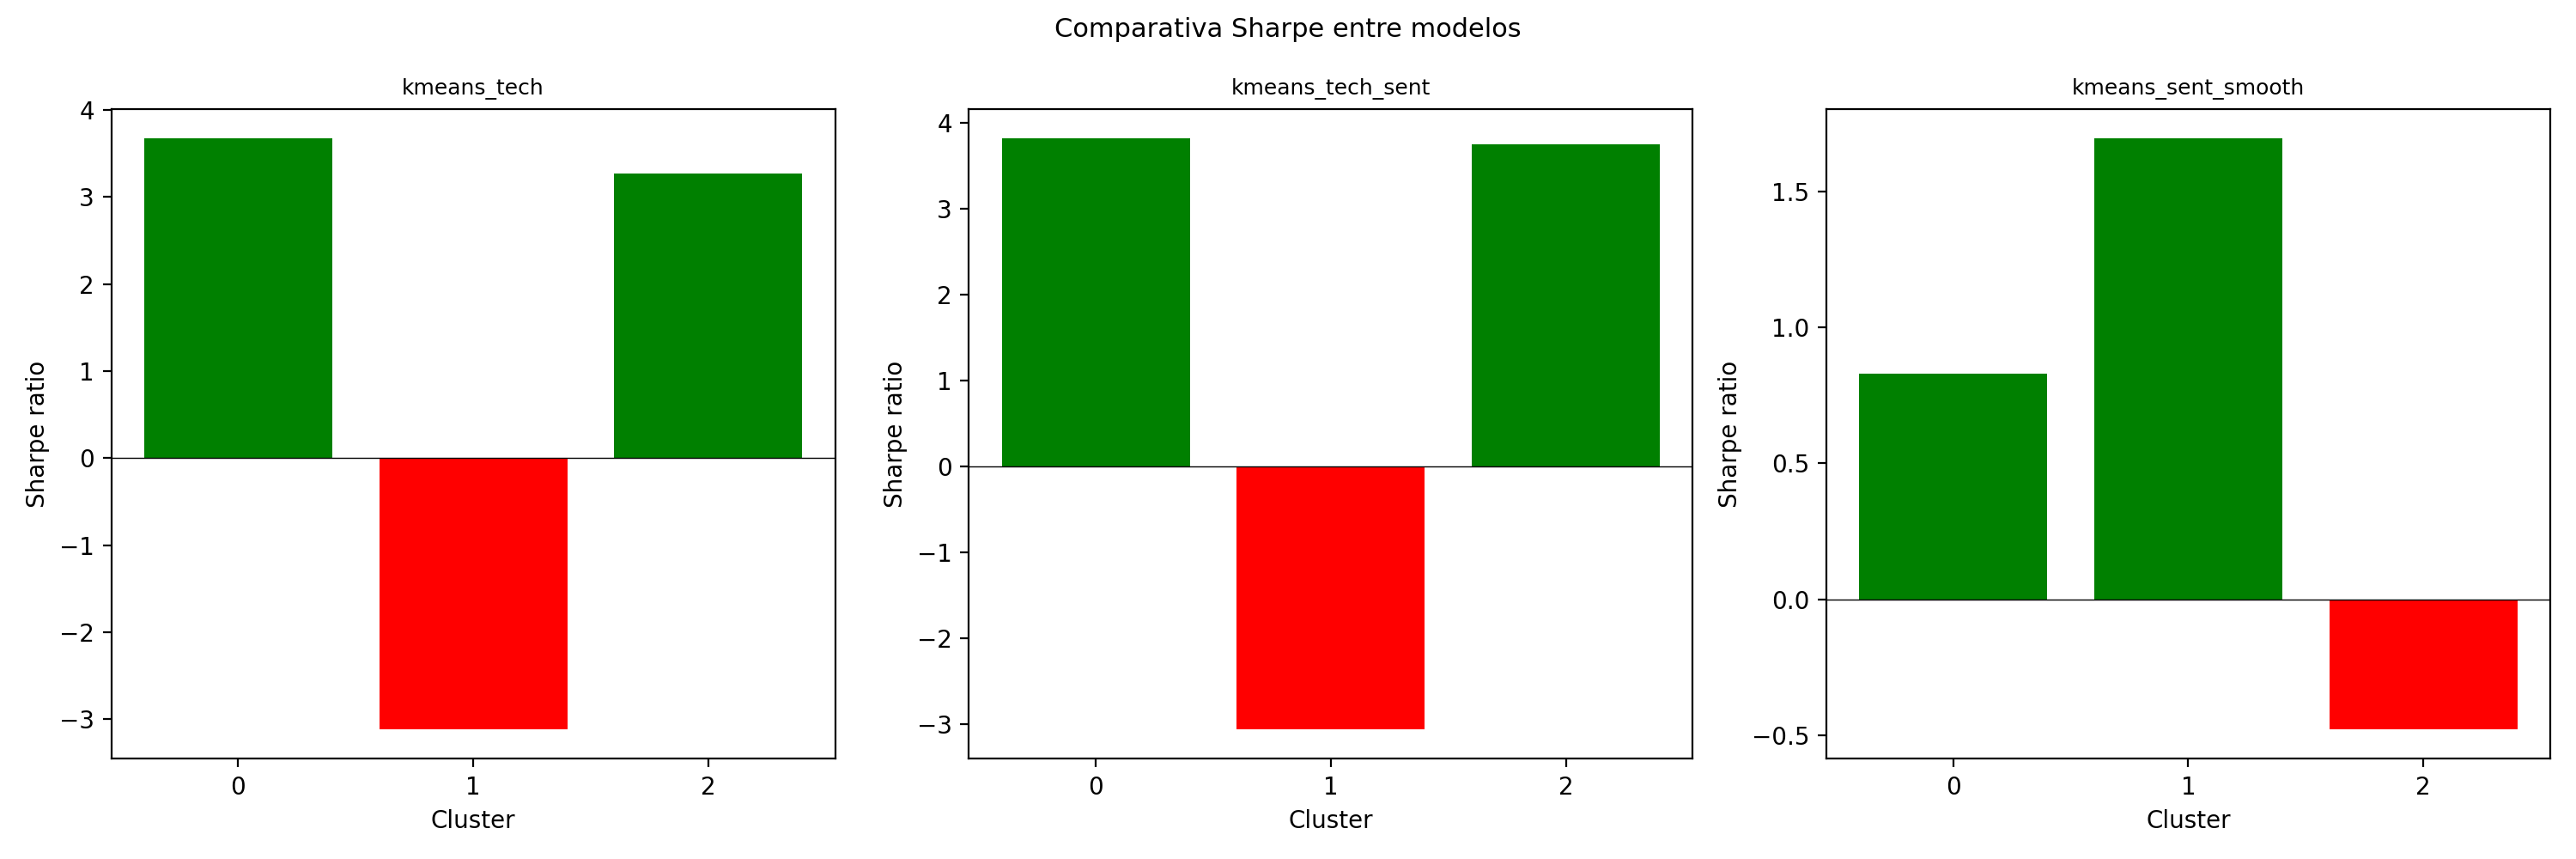
\includegraphics[width=\textwidth]{figures/fig_sharpe_comparativa.png}
  \caption{Market-level Sharpe ratio by cluster for Models A (\texttt{kmeans\_tech}), B (\texttt{kmeans\_tech\_sent}) and C (\texttt{kmeans\_sent\_smooth}). Green bars indicate a positive Sharpe ratio, red bars a negative Sharpe ratio.}
  \label{fig:sharpe-comparativa}
\end{figure}

Taken together, these results constitute a \textbf{meaningful negative
finding}: aggregated sector sentiment, even after MA21 smoothing
specifically designed to capture medium-term trends
(\Cref{sec:meth-smoothing}), does \emph{not}, on its own, recover a
partition of trading days that aligns with either the technical regime
structure or a monotonic economic (Sharpe ratio) ordering. This does not
imply that sentiment is uninformative --- Model B's results
(\Cref{sec:results-econ-sector}) and the feature-importance analysis
(\Cref{sec:results-importance}) show that sentiment-derived features,
particularly \texttt{sentiment\_std} columns, contribute meaningfully
\emph{when combined with} technical features. Rather, it indicates that
sentiment functions as a \emph{complement} to price information, not as a
\emph{substitute} for it, at least at the sector-aggregation and smoothing
granularity considered in this thesis.

\section{K-Means versus Gaussian HMM}
\label{sec:results-hmm}

\Cref{tab:market-hmm} (\Cref{sec:results-econ-overall}) reported the
market-level Sharpe ratios for the two Gaussian HMM variants:
\texttt{hmm\_tech} ($-0.63$ to $+1.54$) and \texttt{hmm\_tech\_sent}
($-0.25$ to $+1.25$). Comparing these ranges to the corresponding
\textit{K-Means} ranges --- $-3.12$ to $+3.68$ for Model A, and $-3.06$ to
$+3.82$ for Model B --- shows that the \textbf{spread of Sharpe ratios
across regimes/states produced by the HMM is roughly 4--5 times narrower
than that produced by K-Means}, for both the technical-only and
technical+sentiment feature sets.

This finding is consistent with the theoretical discussion in
\Cref{sec:soa-hmm}: the HMM's transition matrix imposes \emph{temporal
persistence} on the state sequence (a day is likely to remain in the same
state as the previous day, governed by the diagonal of the transition
matrix), which tends to produce states that are temporal
\emph{aggregates} of more homogeneous sub-periods. \textit{K-Means}, by
contrast, assigns each day independently to the cluster whose centroid it
is closest to in feature space, with no penalty for switching clusters
from one day to the next. As a result, \textit{K-Means} can isolate a
small number of \emph{extreme} days (e.g., Model A's and B's
\emph{Crisis} regime, $n=70$, 6.2\% of the sample) into their own cluster,
producing a centroid --- and therefore an economic profile --- that is
sharply different from the other two clusters. The HMM's states, being
constrained by transition dynamics, instead tend to blend such extreme
days together with the surrounding, less extreme days of the same
\emph{episode}, producing milder, more ``averaged'' state-level
statistics.

From a practical standpoint, this represents a genuine
\textbf{trade-off} rather than a simple ranking of ``better'' versus
``worse'' models. \textit{K-Means}'s sharper regimes are more useful for
\emph{characterizing} what an extreme regime looks like economically
(as in \Cref{sec:results-econ-sector}), since its \emph{Crisis} cluster is
not diluted by adjacent, more moderate days. The HMM's smoother regimes,
on the other hand, may be more directly useful for \emph{real-time
monitoring} or \emph{trading} applications, where a regime indicator that
switches state on every isolated extreme day (as \textit{K-Means} labels
can, since they carry no explicit persistence constraint) would generate
excessive turnover. \Cref{fig:hmm-states-modelA,fig:hmm-states-modelB}
(\Cref{sec:results-regimes}) illustrate this: the HMM states visibly
persist over multi-week to multi-month spans, in line with the
\texttt{vol30d\_sp500} dynamics, whereas the \textit{K-Means}-based regime
shading in \Cref{fig:sp500-regimes-modelA,fig:sp500-regimes-modelB} shows a
\emph{Crisis} regime confined to brief, sharply-defined episodes.

\section{Summary of Key Findings}
\label{sec:results-summary}

The results presented in this chapter can be summarized in five key
findings:

\begin{enumerate}
  \item \textbf{Technical indicators remain the strongest structural
  discriminator}, both in terms of silhouette coefficient in the common
  PCA space (Model A: 0.1928 vs.\ Model B: 0.1778 vs.\ Model C: 0.1623,
  \Cref{tab:silhouette-comparison}) and in terms of ANOVA feature
  importance (the top 6 features for Model B are all technical,
  \Cref{tab:feature-importance}).

  \item \textbf{Sentiment-augmented clustering (Model B) sharpens economic
  differentiation relative to the technical-only baseline (Model A)},
  particularly for the \emph{Bull} and \emph{Crisis} regimes (market-level
  Sharpe of $3.82$ and $3.75$ for Model B vs.\ $3.68$ and $3.28$ for Model
  A), while the \emph{Bear} regime becomes negative across nearly all
  sectors (10 of 11) under Model B.

  \item \textbf{The \emph{Bear} regime is the only regime with negative
  Sharpe ratios at both the market and (almost universally) the sector
  level}, while the \emph{Crisis} regime --- despite having the highest
  volatility --- has the \emph{highest} Sharpe ratios across all sectors,
  reflecting its association with sharp V-shaped recoveries (2009, 2020)
  rather than sustained losses.

  \item \textbf{The \emph{Energy} sector in the \emph{Bear} regime is the
  single most extreme combination in the dataset}: it has the worst
  maximum drawdown ($-74.9\%$) of any sector/regime combination, and
  contains both the best ($+16.9\%$) and the worst ($-24.7\%$) single-day
  returns of the entire sample.

  \item \textbf{Sentiment alone (Model C) is not a viable substitute for
  technical indicators}: its cluster centroids are nearly
  indistinguishable in technical-feature space, and its inherited
  Bull/Bear/Crisis labels do not preserve a monotonic Sharpe-ratio
  ordering. \textbf{The Gaussian HMM produces qualitatively similar but
  quantitatively much milder regimes than K-Means} (Sharpe ratio ranges
  roughly 4--5 times narrower), reflecting the trade-off between temporal
  persistence and sharp economic differentiation.
\end{enumerate}

These findings are discussed further, together with their limitations and
implications for future work, in \Cref{ch:conclusions}.

\chapter{Conclusions and Future Work}
\label{ch:conclusions}

This final chapter synthesizes the work presented in this thesis.
\Cref{sec:concl-summary} summarizes the pipeline that was designed and
implemented. \Cref{sec:concl-findings} revisits the central research
question posed in \Cref{ch:introduction} in light of the results of
\Cref{ch:results}. \Cref{sec:concl-limitations} discusses the limitations
of the methodology, and \Cref{sec:concl-future} outlines directions for
future work.

\section{Summary of the Thesis}
\label{sec:concl-summary}

This thesis set out to answer the following question: \emph{can
sector-level sentiment extracted from financial news using FinBERT improve
the identification of market regimes obtained through unsupervised
clustering of technical indicators, and if so, in what sense?}
(\Cref{sec:motivation}). To answer it, a complete, reproducible
end-to-end pipeline was designed and implemented, comprising:

\begin{itemize}
  \item \textbf{Data acquisition and filtering} (\Cref{sec:meth-fnspid,sec:meth-sp500,sec:meth-filtering}):
  financial news headlines from the FNSPID corpus were filtered to retain
  only those associated with companies that were S\&P 500 constituents at
  the time of publication, and reassigned to the next open trading day to
  prevent look-ahead bias.

  \item \textbf{Sentiment scoring with FinBERT} (\Cref{sec:meth-finbert}):
  each filtered headline was scored with the \texttt{ProsusAI/finbert}
  model, producing a continuous score $s = p_{\text{pos}} - p_{\text{neg}}
  \in [-1,1]$ and a categorical label.

  \item \textbf{Sector-level aggregation and smoothing}
  (\Cref{sec:meth-aggregation,sec:meth-smoothing}): scores were aggregated
  by (date, GICS sector) into mean and standard deviation statistics, and
  a 21-session moving average was applied, reducing day-to-day noise by
  47.4--72.6\% depending on the sector while preserving medium-term trends
  (\Cref{tab:ma-noise-reduction}).

  \item \textbf{Technical indicator computation}
  (\Cref{sec:meth-technical}): nine indicators (RSI, two moving-average
  ratios, two momentum measures, two realized-volatility measures and two
  skewness measures) were computed from daily S\&P 500 OHLC prices.

  \item \textbf{Dataset construction} (\Cref{sec:meth-dataset}): technical
  and sentiment features were merged into a single daily dataset of 1,132
  observations (May 2009 -- February 2024, 46 columns).

  \item \textbf{Clustering} (\Cref{sec:meth-kmeans,sec:meth-hmm}): three
  \textit{K-Means} configurations (Model A -- technical only; Model B --
  technical + raw sentiment; Model C -- smoothed sentiment only), each
  with $K=3$, plus a Gaussian HMM ($K=3$, full covariance) fitted on the
  Model A and Model B feature sets, were trained and the resulting
  clusters/states labeled as \emph{Bull}, \emph{Bear} or \emph{Crisis}
  via centroid analysis (\Cref{sec:meth-labeling}).

  \item \textbf{Internal and economic validation}
  (\Cref{sec:meth-validation,ch:results}): the resulting partitions were
  evaluated through silhouette analysis in a common PCA space,
  ANOVA-based feature importance, and a sector-level economic validation
  framework computing annualized return, volatility, Sharpe ratio,
  maximum drawdown, percentage of positive days, and extreme daily returns
  for every (GICS sector, regime) combination.
\end{itemize}

\section{Main Findings and Answer to the Research Question}
\label{sec:concl-findings}

The results of \Cref{ch:results} support a nuanced, two-part answer to the
thesis's central question.

\textbf{On purely statistical (internal) grounds, sentiment does not
improve cluster cohesion.} The silhouette coefficient computed in a common
9-component PCA space (82.0\% explained variance) ranks Model A
(technical only, $0.1928$) above Model B (technical + raw sentiment,
$0.1778$), which in turn ranks above Model C (smoothed sentiment only,
$0.1623$) (\Cref{tab:silhouette-comparison}). Moreover, the ANOVA
feature-importance analysis (\Cref{tab:feature-importance}) confirms that
the six most discriminative features for Model B's partition are all
technical indicators, with \texttt{MA50\_ratio\_sp500} ($F=597.81$) and
\texttt{RSI\_sp500} ($F=561.49$) leading by a wide margin. Technical
indicators therefore remain the primary axis along which the data
naturally separates into clusters.

\textbf{However, on economic grounds, incorporating sentiment sharpens the
differentiation between regimes.} Model B's \emph{Bear} regime exhibits a
negative Sharpe ratio in 10 of the 11 GICS sectors
(\Cref{fig:heatmap-sharpe-modelB}), compared to a qualitatively similar but
slightly less extreme pattern for Model A
(\Cref{fig:heatmap-sharpe-modelA}). At the market level, Model B's
\emph{Bull} and \emph{Crisis} Sharpe ratios ($3.82$ and $3.75$) are both
higher than Model A's ($3.68$ and $3.28$), while its \emph{Bear} Sharpe
($-3.06$) is marginally less negative than Model A's ($-3.12$)
(\Cref{tab:market-kmeans}). The net effect of adding raw sector sentiment
to the feature set is thus a partition that is statistically slightly less
cohesive, but economically slightly \emph{more} differentiated --- a
trade-off that, in the context of regime detection for risk management or
asset allocation, may reasonably be considered favorable, since the
economic interpretability of a regime (how different is its Sharpe ratio
from the others?) is arguably more decision-relevant than its purely
geometric cohesion in feature space.

A second major finding concerns \textbf{what each regime represents
economically}. Across Models A and B, the \emph{Bear} regime is the only
one with a negative aggregate Sharpe ratio, and is associated with deep
drawdowns (mean across sectors of $-47.2\%$ for Model B). The
\emph{Crisis} regime, despite having the highest point-in-time volatility,
has the \emph{highest} Sharpe ratio of the three regimes for every single
GICS sector, reflecting its association with the sharp V-shaped recoveries
that followed the 2008--2009 financial crisis and the 2020 COVID-19 crash
(\Cref{sec:results-regimes}). The single most extreme sector/regime
combination in the entire dataset is \emph{Energy} during the \emph{Bear}
regime, which records the worst maximum drawdown ($-74.9\%$) and both the
best ($+16.9\%$) and worst ($-24.7\%$) single-day returns of the whole
sample (\Cref{fig:heatmap-maxdd-modelB,fig:heatmap-bestday-modelB,fig:heatmap-worstday-modelB}).

A third finding is the \textbf{negative result associated with Model C}
(\Cref{sec:results-modelC}): clustering on smoothed sector sentiment alone
produces clusters whose technical centroids are nearly indistinguishable
(e.g., \texttt{MA50\_ratio\_sp500} ranges only from $1.0086$ to $1.0134$
across Model C's three clusters, versus a range of $0.0653$ for Model A),
and whose inherited Bull/Bear/Crisis labels do not preserve a monotonic
Sharpe-ratio ordering (Model C's ``Bear'' regime has a \emph{higher}
market-level Sharpe ratio than its ``Bull'' regime). This indicates that,
at the sector-aggregation and 21-session smoothing granularity considered
in this thesis, sentiment functions as a \emph{complement} to price
information rather than a \emph{substitute} for it.

Finally, the \textbf{comparison between \textit{K-Means} and the Gaussian
HMM} (\Cref{sec:results-hmm}) shows that both methods identify
qualitatively similar regimes --- both isolate a small, high-volatility
cluster/state associated with 2009 and 2020 --- but the HMM's
state-level Sharpe ratios ($-0.63$ to $+1.54$ for \texttt{hmm\_tech},
$-0.25$ to $+1.25$ for \texttt{hmm\_tech\_sent}) span a range roughly
4--5 times narrower than \textit{K-Means}'s ($-3.12$ to $+3.82$). This is
attributed to the temporal-persistence constraint imposed by the HMM's
transition matrix, which causes extreme days to be ``averaged'' together
with the surrounding, less extreme days of the same episode --- a
trade-off between temporal coherence and sharp economic differentiation
that should inform the choice of method depending on the intended
application (real-time monitoring versus retrospective characterization of
regimes).

In summary, this thesis concludes that \textbf{sector-level sentiment
extracted via FinBERT does not, by itself, define market regimes as
sharply as technical indicators, but when combined with technical
indicators, it produces regimes with a sharper and more
sector-consistent economic profile} --- in particular, a more uniformly
adverse \emph{Bear} regime across the equity market. This constitutes a
modest but genuine affirmative answer to the thesis's central question,
while also identifying a clear boundary condition (Model C) beyond which
sentiment alone is insufficient.

\section{Limitations}
\label{sec:concl-limitations}

Several limitations of the methodology adopted in this thesis should be
acknowledged.

\begin{enumerate}
  \item \textbf{Survivorship and constituent-list bias.} The S\&P 500
  constituent list used to filter FNSPID news reflects, for practical
  reasons, a snapshot-based approach to historical membership
  (\Cref{sec:meth-sp500}). Companies that were removed from the index
  (e.g., due to bankruptcy or acquisition) may be under-represented in the
  news-filtering step for the periods immediately preceding their removal,
  which could introduce a mild positive bias in the sentiment signal
  associated with distressed companies.

  \item \textbf{Sector-level aggregation discards firm-level information.}
  By aggregating sentiment at the GICS sector level, the pipeline
  necessarily discards information about \emph{which} companies within a
  sector are driving the sentiment signal on a given day. A small number
  of highly-covered companies (e.g., large-cap technology firms within
  \textit{Information Technology}) may disproportionately influence the
  sector-level average, effectively making the sector signal a
  weighted-by-news-volume proxy for its most newsworthy constituents
  rather than a balanced sector-wide measure.

  \item \textbf{Dataset size and the curse of dimensionality for Model B.}
  Model B's 31-dimensional feature space (9 technical + 22 raw sentiment
  features) is clustered using only 1,132 observations --- a
  feature-to-observation ratio that, while not unusual for exploratory
  cluster analysis, may make the resulting partition more sensitive to
  noise in the raw (unsmoothed) sentiment columns than a model with fewer
  features. This is reflected in Model B's comparatively low silhouette
  coefficient in its own feature space (0.1213, \Cref{tab:silhouette-comparison}).

  \item \textbf{Methodological discrepancy in the MA21 justification
  analysis.} As discussed in \Cref{sec:meth-smoothing}, the noise-reduction
  analysis that motivated the choice of a 21-session moving average
  (\Cref{tab:ma-noise-reduction}) was performed on an earlier snapshot of
  the sentiment dataset (1,073 observations, 2009--2019) rather than on the
  final 1,132-observation dataset (2009--2024) used for clustering. While
  there is no reason to expect the qualitative conclusion (MA21 provides
  substantial noise reduction while preserving medium-term trends) to
  change with the additional 2019--2024 data, the exact noise-reduction
  percentages reported were not recomputed on the final dataset.

  \item \textbf{Fixed number of clusters/states ($K=3$).} All clustering
  models in this thesis use $K=3$, motivated by the conventional
  Bull/Bear/Crisis trichotomy. While this choice is supported by the elbow
  method for Models A and B (\Cref{fig:elbow-modelA,fig:elbow-modelB}), it
  was not exhaustively re-validated for Model C or for the HMM, and a
  different value of $K$ might reveal additional, economically meaningful
  sub-regimes (e.g., a separate ``recovery'' regime distinct from
  ``crisis'').

  \item \textbf{Single asset universe and time period.} The analysis is
  restricted to S\&P 500 constituents over a single 15-year period
  (2009--2024), which is dominated by a long secular bull market punctuated
  by two major crisis episodes (2009, 2020). The generalizability of the
  findings --- particularly the relative ranking of Models A, B and C ---
  to other equity markets, other asset classes (e.g., fixed income,
  commodities), or different macroeconomic regimes (e.g., a sustained
  high-inflation environment) has not been tested.

  \item \textbf{Static, unsupervised evaluation.} The economic validation
  framework (\Cref{sec:meth-validation}) computes \emph{retrospective}
  performance metrics for days already assigned to a given regime; it does
  not evaluate whether the detected regimes could have been identified
  \emph{in real time}, nor does it assess the practical profitability of a
  trading or risk-management strategy that would have reacted to regime
  transitions as they occurred.
\end{enumerate}

\section{Future Work}
\label{sec:concl-future}

Building on the findings and limitations discussed above, several
directions for future work can be identified.

\begin{itemize}
  \item \textbf{Firm-level sentiment features.} Rather than aggregating
  sentiment only at the GICS sector level, future work could retain
  firm-level sentiment scores (or a small number of summary statistics per
  firm) and incorporate cross-sectional dispersion measures --- e.g., the
  fraction of constituent firms within a sector with strongly negative
  sentiment on a given day --- which may carry information that is averaged
  away by sector-level aggregation.

  \item \textbf{Dynamic / adaptive number of clusters.} The fixed choice of
  $K=3$ could be relaxed by exploring model-selection criteria (e.g.,
  Bayesian Information Criterion for the HMM, or gap-statistic-based
  selection for \textit{K-Means}) applied independently to each of Models
  A, B and C, to test whether the technical+sentiment feature space
  naturally supports a different number of regimes than the technical-only
  space.

  \item \textbf{Sequential and deep-learning architectures.} The
  comparison between \textit{K-Means} (sharp, non-temporal) and the
  Gaussian HMM (smooth, temporal but Gaussian-emission) could be extended
  to more flexible sequential models, such as recurrent neural networks,
  Transformer-based sequence models, or non-Gaussian HMM variants (e.g.,
  with Student-$t$ or mixture emissions), which might combine the temporal
  coherence of the HMM with the sharper economic differentiation of
  \textit{K-Means}.

  \item \textbf{Real-time / online regime detection.} The current pipeline
  operates in a fully \emph{retrospective} (batch) setting. An important
  extension would be to implement an online or rolling-window version of
  the pipeline, in which sentiment scores, technical indicators and
  cluster/state assignments are updated incrementally as new data arrives,
  and to evaluate the \emph{lead time} between a regime transition being
  detected and the corresponding shift in aggregate market returns.

  \item \textbf{Trading and risk-management applications.} A natural
  extension of the economic validation framework would be to design and
  backtest simple rule-based strategies that adjust sector exposure based
  on the detected regime (e.g., reducing exposure to sectors in their
  \emph{Bear} regime), accounting for transaction costs and
  implementation lags, to assess whether the economic differentiation
  documented in \Cref{ch:results} translates into a practically
  exploitable signal.

  \item \textbf{Extension to other markets and asset classes.} Repeating
  the pipeline for other equity indices (e.g., European or Asian
  benchmarks), for individual large-cap stocks, or for other asset classes
  such as government bonds or commodities, would help establish whether
  the incremental value of sentiment documented for the S\&P 500 in this
  thesis generalizes, or whether it is specific to the news coverage
  patterns and market dynamics of US large-cap equities.

  \item \textbf{Updated MA21 justification on the final dataset.} As noted
  in \Cref{sec:concl-limitations}, the moving-average noise-reduction
  analysis of \Cref{tab:ma-noise-reduction} could be recomputed on the
  final 1,132-observation (2009--2024) dataset, both to confirm the
  reported noise-reduction percentages and to verify that the choice of a
  21-session window remains optimal once the additional 2019--2024 data is
  included.
\end{itemize}

Taken together, these directions point towards a broader research program
in which sentiment-augmented, unsupervised regime detection is developed
from the exploratory, retrospective analysis presented in this thesis into
a more granular, adaptive, and ultimately actionable tool for
understanding and responding to changes in market conditions.


% ------------------------------------------------------------
% BIBLIOGRAPHY
% ------------------------------------------------------------
\printbibliography[heading=bibintoc,title={Bibliography}]

% ------------------------------------------------------------
% ANNEXES
% ------------------------------------------------------------
\appendix
\chapter{Pipeline Source Code Structure}
\label{annex:pipeline}

This annex describes the organization of the source code repository
implementing the data pipeline described in \Cref{ch:methodology}. All
code is written in Python, using \texttt{pandas} and \texttt{numpy} for
data manipulation, \texttt{yfinance} for market data retrieval,
\texttt{Hugging Face transformers} and \texttt{torch} for FinBERT
inference, and \texttt{scikit-learn} / \texttt{hmmlearn} for clustering.
The repository is organized into four top-level packages under
\texttt{src/}, corresponding to the four major stages of the pipeline:
\texttt{news}, \texttt{market}, \texttt{sentiment} and \texttt{clustering},
plus an \texttt{eda} package containing exploratory analyses that informed
several methodological decisions (e.g., the choice of the MA21 smoothing
window in \Cref{sec:meth-smoothing}).

\section{Repository Structure}
\label{annex:pipeline-structure}

\begin{verbatim}
src/
├── news/
│   └── load_fnspid.py            Stream and cache the raw FNSPID corpus
├── market/
│   ├── download_sp500.py         Download S&P 500 OHLC prices (yfinance)
│   ├── sp500_historical.py        Historical S&P 500 constituents lookup
│   └── technical_indicators.py    Compute the 9 technical indicators
├── sentiment/
│   ├── sentiment_finbert.py       FinBERT batched sentiment scoring
│   ├── aggregate_sentiment.py     (date, ticker)-level aggregation
│   ├── aggregate_by_sector.py     (date, sector)-level aggregation + MA21
│   ├── cross_market_sentiment.py  Merge sentiment with market returns
│   └── build_clustering_dataset.py  Final clustering dataset assembly
├── eda/
│   ├── eda_gics_mapping.py         Build ticker -> GICS sector mapping
│   ├── eda_filter_sp500_news.py    Filter FNSPID news by S&P 500 membership
│   ├── eda_ticker_quality.py       Per-ticker news coverage diagnostics
│   ├── eda_news.py                 News volume / distribution analyses
│   ├── eda_market.py               Market data quality checks
│   ├── eda_news_vs_market.py       News vs. market exploratory analysis
│   ├── eda_fnspid_full_stream_analysis.py  Full-corpus FNSPID statistics
│   └── eda_sentiment_smoothing.py  MA5/MA10/MA21 noise-reduction analysis
└── clustering/
    ├── clustering.py               K-Means Models A/B/C + Gaussian HMM
    ├── silhouette_pca.py           PCA-common-space silhouette comparison
    ├── feature_importance.py       ANOVA F-statistic feature importance
    ├── plot_clusters.py             PCA, correlation and regime plots
    ├── economic_validation.py       Market-level economic metrics
    └── sector_regime_analysis.py    Sector-level economic metrics & heatmaps
\end{verbatim}

Each module follows the same general convention: input and output paths
are defined as module-level constants (typically under \texttt{data/raw/},
\texttt{data/processed/} or \texttt{outputs/}), and a \texttt{main()}
function executes the corresponding processing step, printing progress
information (row counts, date ranges, intermediate statistics) to allow
each stage to be run and verified independently. The following sections
describe each stage in more detail.

\section{Data Acquisition}
\label{annex:pipeline-acquisition}

\textbf{\texttt{news/load\_fnspid.py}} streams the FNSPID dataset
(\texttt{Zihan1004/FNSPID} on the Hugging Face Hub, corresponding to
\cite{zhang2023fnspid}) using the \texttt{datasets} library in streaming
mode, and writes the relevant columns (publication date, headline title,
stock ticker, publisher and URL) to a local CSV cache under
\texttt{data/raw/news/}. Streaming mode is used because the full corpus
contains several million rows and does not fit comfortably in memory.

\textbf{\texttt{market/download\_sp500.py}} downloads daily OHLC
(open/high/low/close/volume) data for the S\&P 500 index from Yahoo
Finance via \texttt{yfinance}, with a retry mechanism (up to 3 attempts per
ticker) to handle transient network failures, and caches the result under
\texttt{data/raw/market/}.

\textbf{\texttt{market/sp500\_historical.py}} provides a lookup function,
\texttt{sp500\_tickers\_on(date)}, which, given a \texttt{data/raw/market/sp500\_historical\_components.csv}
file containing the historical list of S\&P 500 constituents at successive
dates, returns the list of tickers that were constituents of the index on
(or most recently before) a given date. This function underpins the
membership-filtering step described in \Cref{sec:meth-sp500}.

\section{News Filtering and GICS Sector Mapping}
\label{annex:pipeline-filtering}

\textbf{\texttt{eda/eda\_gics\_mapping.py}} constructs a
ticker-to-GICS-sector mapping (\texttt{data/raw/market/ticker\_gics\_mapping.csv})
by combining a base table of known sectors with sector information
retrieved from Yahoo Finance for any remaining tickers, and normalizes
Yahoo Finance's sector names to the standard GICS sector names used
throughout this thesis (e.g., \texttt{"Healthcare"} $\to$ \texttt{"Health
Care"}, \texttt{"Financials"} $\to$ \texttt{"Financial Services"},
\texttt{"Consumer Cyclical"} $\to$ \texttt{"Consumer Discretionary"},
\texttt{"Consumer Defensive"} $\to$ \texttt{"Consumer Staples"},
\texttt{"Basic Materials"} $\to$ \texttt{"Materials"}, \texttt{"Technology"}
$\to$ \texttt{"Information Technology"}), producing the 11-sector
distribution summarized in \Cref{tab:gics-distribution}.

\textbf{\texttt{eda/eda\_filter\_sp500\_news.py}} implements the
membership-filtering step of \Cref{sec:meth-filtering}: it expands the
historical S\&P 500 constituents table into a long (date, ticker) table,
and retains only those FNSPID news rows whose (date, ticker) pair appears
in this table --- i.e., news items associated with a company that was an
S\&P 500 constituent on the date the news was published. The filtered
result is written to \texttt{data/processed/news/fnspid\_sp500.parquet}.

\section{FinBERT Sentiment Scoring}
\label{annex:pipeline-finbert}

\textbf{\texttt{sentiment/sentiment\_finbert.py}} implements the sentiment
scoring procedure of \Cref{sec:meth-finbert}. After loading the filtered
news parquet, normalizing column names (\texttt{date}, \texttt{ticker},
\texttt{title}) and dropping unused summary columns, the script loads the
\texttt{ProsusAI/finbert} model via the \texttt{transformers.pipeline} API
(using GPU acceleration when available, \texttt{torch.cuda.is\_available()}),
and processes all headlines in batches of \texttt{BATCH\_SIZE = 64}. Each
headline is truncated to 512 characters before tokenization (FinBERT's
maximum input length). For each headline, the pipeline returns class
probabilities $p_{\text{pos}}, p_{\text{neg}}, p_{\text{neu}}$, from which
the continuous sentiment score $s = p_{\text{pos}} - p_{\text{neg}}$
(\Cref{eq:sentiment-score}) and the categorical label
(\Cref{eq:sentiment-label}) are derived. The module also supports a
\texttt{DEBUG\_MODE} flag that restricts processing to a random subset of
50,000 headlines (\texttt{random\_state=42}) for fast iteration during
development; all results reported in this thesis use the full corpus
(\texttt{DEBUG\_MODE = False}).

\section{Sector-Level Aggregation and Smoothing}
\label{annex:pipeline-aggregation}

\textbf{\texttt{sentiment/aggregate\_sentiment.py}} performs an
intermediate (date, ticker)-level aggregation, computing, for each
ticker and day, the mean and standard deviation of the sentiment score
across all headlines published that day (\texttt{sentiment\_score\_mean},
\texttt{sentiment\_score\_std}), the total number of news items, and the
counts of positive/negative/neutral headlines.

\textbf{\texttt{sentiment/aggregate\_by\_sector.py}} performs the
sector-level aggregation described in \Cref{sec:meth-aggregation}: it
merges the per-ticker sentiment scores with the GICS sector mapping
(an inner join on \texttt{ticker}), groups by \texttt{(date, sector)}, and
computes \texttt{sentiment\_avg} (mean) and \texttt{sentiment\_std}
(standard deviation, \Cref{eq:sector-mean,eq:sector-std}) of the sentiment
score across all news items published about companies in that sector on
that day. Standard deviations for (date, sector) cells with a single news
item (undefined sample standard deviation) are filled with zero. The
resulting long table is then pivoted into a wide format with one column
per (statistic, sector) combination, and a rolling mean with
\texttt{SMOOTH\_WINDOW = 21} sessions (\Cref{eq:ma-smooth}) is applied to
each \texttt{sentiment\_avg} column to produce the corresponding
\texttt{\_smooth} columns used by Model C.

\textbf{\texttt{sentiment/cross\_market\_sentiment.py}} is an exploratory
module that merges the aggregated per-ticker sentiment series with daily
S\&P 500 returns and rolling volatility, used during the EDA phase to
visualize the relationship between sentiment and market dynamics
(\Cref{sec:soa-gap}); it is not part of the critical path that produces the
final clustering dataset.

\section{Technical Indicators}
\label{annex:pipeline-technical}

\textbf{\texttt{market/technical\_indicators.py}} computes the 9 technical
indicators of \Cref{sec:meth-technical} from the daily S\&P 500 OHLC
series. Log returns are computed as
$r_t = \ln(\text{close}_t / \text{close}_{t-1})$. The Relative Strength
Index is computed via \texttt{compute\_rsi()}, using exponentially-weighted
moving averages of gains and losses with a center-of-mass parameter
\texttt{com = window - 1} for a 14-session window
(\Cref{eq:rsi}). The 50- and 200-session moving-average ratios
(\texttt{MA50\_ratio}, \texttt{MA200\_ratio}, \Cref{eq:ma-ratio}), the
21- and 126-session momentum measures (\texttt{mom21}, \texttt{mom126},
\Cref{eq:momentum}), and the 30- and 252-session annualized realized
volatilities (\texttt{vol\_30d}, \texttt{vol\_252d}, scaled by
$\sqrt{252}$, \Cref{eq:realized-vol}) and rolling skewness measures
(\texttt{skew\_30d}, \texttt{skew\_252d}, \Cref{eq:skewness}) are computed
using \texttt{pandas} rolling-window operations on the log-return series.

\section{Clustering Dataset Construction}
\label{annex:pipeline-dataset}

\textbf{\texttt{sentiment/build\_clustering\_dataset.py}} performs the
final assembly step of \Cref{sec:meth-dataset}. It loads the sector-level
sentiment table and the technical indicator table, renames the technical
columns with the \texttt{\_sp500} suffix (e.g., \texttt{RSI} $\to$
\texttt{RSI\_sp500}), drops auxiliary columns (\texttt{ret}, \texttt{close})
that are not used as clustering features, and performs an inner merge on
\texttt{date}. A date cutoff (\texttt{DATE\_CUTOFF}) is applied to exclude
incomplete trailing observations, and rows with missing values --- arising
from the warm-up periods required by the longest rolling windows
(252 sessions for \texttt{vol252d\_sp500} and \texttt{skew252d\_sp500}) ---
are dropped, yielding the final 1{,}132-observation, 46-column dataset
written to \texttt{data/processed/clustering\_dataset.parquet}.

\section{Clustering, Internal Validation and Economic Validation}
\label{annex:pipeline-clustering}

\textbf{\texttt{clustering/clustering.py}} is the central module of the
clustering stage. It defines the three feature sets \texttt{FEATURES\_TECH}
(9 technical features, Model A), \texttt{FEATURES\_ALL} (\texttt{FEATURES\_TECH}
plus the 22 raw sentiment columns, Model B) and the 11 MA21-smoothed
sentiment columns (Model C), standardizes each feature set with
\texttt{StandardScaler}, and fits \texttt{sklearn.cluster.KMeans} with
$K=3$ for each of the three configurations (\Cref{eq:soa-kmeans-objective}),
storing the resulting labels as \texttt{kmeans\_tech}, \texttt{kmeans\_tech\_sent}
and \texttt{kmeans\_sent\_smooth} columns in
\texttt{outputs/clustering/clustered\_data.parquet}. The same module also
implements \texttt{run\_hmm()}, which fits
\texttt{hmmlearn.hmm.GaussianHMM(n\_components=3, covariance\_type="full",
n\_iter=1000, random\_state=42, min\_covar=1e-3)} on the standardized
\texttt{FEATURES\_TECH} and \texttt{FEATURES\_ALL} feature sets, producing
the \texttt{hmm\_tech} and \texttt{hmm\_tech\_sent} state assignments via
\texttt{model.predict()}, and saves a diagnostic plot of 30-day realized
volatility colored by HMM state
(\Cref{fig:hmm-states-modelA,fig:hmm-states-modelB}).

\textbf{\texttt{clustering/silhouette\_pca.py}} implements the
common-PCA-space silhouette comparison of
\Cref{sec:results-silhouette}: it standardizes the union of the 9 technical
and 11 smoothed sentiment features (20 features), fits a PCA retaining
components up to 80\% explained variance (9 components, 82.0\% actual
variance), projects each of the three K-Means partitions into this common
space, and computes the silhouette coefficient
(\Cref{eq:soa-silhouette}) of each partition in the projected space, saving
\texttt{fig\_silhouette\_pca\_comparison.png} and \texttt{fig\_silhouette\_scree.png}.

\textbf{\texttt{clustering/feature\_importance.py}} computes, for the
Model B partition (\texttt{kmeans\_tech\_sent}), the ANOVA F-statistic of
each of the 31 input features with respect to the 3-cluster grouping
using \texttt{sklearn.feature\_selection.f\_classif}, ranks the features by
F-statistic, and saves the results to
\texttt{outputs/clustering/validation/feature\_importance.csv} and
\texttt{fig\_feature\_importance.png} (\Cref{tab:feature-importance,fig:feature-importance}).

\textbf{\texttt{clustering/plot\_clusters.py}} centralizes the visual
diagnostics shared across models: it defines the
\texttt{CLUSTER\_COLORS} mapping ($\{0:\texttt{\#0D7A3E}$ (Bull, green),
$1:\texttt{\#C0392B}$ (Bear, red), $2:\texttt{\#E67E22}$ (Crisis, orange)$\}$)
and \texttt{CLUSTER\_NAMES} mapping used consistently across all figures in
this thesis, and implements \texttt{plot\_pca\_clusters()} (PCA scatter +
loadings + scree plot, \Cref{fig:pca-modelA,fig:pca-modelB}),
\texttt{plot\_sp500\_regimes()} (S\&P 500 price series with regime-shaded
background, \Cref{fig:sp500-regimes-modelA,fig:sp500-regimes-modelB}) and
\texttt{plot\_correlation\_matrix()} (feature correlation heatmaps,
\Cref{fig:correlation-modelA,fig:correlation-modelB}).

\textbf{\texttt{clustering/economic\_validation.py}} implements the
market-level economic validation framework of \Cref{sec:meth-validation}:
for each clustering configuration (Models A, B, C and both HMM variants)
and each regime/state label, it computes the mean daily return, the
annualized return (\Cref{eq:ann-return}), the annualized volatility
(\Cref{eq:ann-vol}), the Sharpe ratio with $r_f = 2\%$
(\Cref{eq:sharpe}), the percentage of positive days, and the best and worst
single-day returns, on the \emph{aggregate} S\&P 500 return series,
writing one CSV file per configuration to
\texttt{outputs/clustering/validation/} (e.g.,
\texttt{metrics\_kmeans\_tech\_sent.csv}, \texttt{metrics\_hmm\_tech.csv}),
summarized in \Cref{tab:market-kmeans,tab:market-hmm}.

\textbf{\texttt{clustering/sector\_regime\_analysis.py}} extends the
economic validation to the sector level (\Cref{sec:results-econ-sector}).
For each of the three K-Means models, it defines a \texttt{MODELS}
configuration dictionary and a \texttt{REGIME\_MAP = \{0: "Bull", 1:
"Bear", 2: "Crisis"\}} label mapping, reindexes the 1{,}132-observation
cluster labels onto the daily calendar of each of the 11 GICS sector return
series via forward-fill (yielding 3{,}695 sector-days per model,
\Cref{sec:results-econ-sector}), computes the same set of economic metrics
plus the maximum drawdown over (non-contiguous) regime days
(\Cref{eq:max-dd}) for every (sector, regime) combination, and writes the
results to \texttt{outputs/clustering/validation/<model>/sector\_regime\_metrics.csv}
(reproduced in full in \Cref{annex:tables}). The function
\texttt{generate\_heatmaps()} then produces, for each model, seven heatmap
figures (Sharpe ratio, maximum drawdown, percentage of positive days, best
day, worst day, annualized return and annualized volatility, by sector and
regime), of which the Sharpe ratio, maximum drawdown, best-day and
worst-day heatmaps for Model B and the Sharpe ratio heatmaps for Models A
and C are reproduced in \Cref{sec:results-econ-sector,sec:results-modelC}.

\chapter{Full Sector-Level Economic Validation Tables}
\label{annex:tables}

This annex reproduces, in full, the sector-level economic validation
tables produced by \texttt{clustering/sector\_regime\_analysis.py}
(\Cref{annex:pipeline-clustering}) for Models A, B and C, summarized in
\Cref{sec:results-econ-sector,sec:results-modelC}. For each of the 11 GICS
sectors and each of the three regimes (\emph{Bull}, \emph{Bear},
\emph{Crisis}), the following metrics are reported: annualized return
(\Cref{eq:ann-return}), annualized volatility (\Cref{eq:ann-vol}), Sharpe
ratio with $r_f = 2\%$ (\Cref{eq:sharpe}), maximum drawdown over
(non-contiguous) regime days (\Cref{eq:max-dd}), the percentage of days
with a positive return, the best and worst single-day returns, and the
number of sector-days assigned to that regime ($n$). All return, volatility
and drawdown figures are expressed as percentages.

\section{Model A (Technical Only, \texttt{kmeans\_tech})}
\label{annex:tables-modelA}

\begin{landscape}
\begin{longtable}{llrrrrrrrr}
\caption{Sector-level economic validation metrics, Model A (\texttt{kmeans\_tech}).}
\label{tab:annexB-modelA}\\
\toprule
\textbf{Sector} & \textbf{Regime} & \textbf{Ret.\ (\%)} & \textbf{Vol.\ (\%)} & \textbf{Sharpe} & \textbf{Max DD (\%)} & \textbf{\% Pos.} & \textbf{Best (\%)} & \textbf{Worst (\%)} & \textbf{$n$} \\
\midrule
\endfirsthead
\multicolumn{10}{c}{\tablename\ \thetable{} -- continued} \\
\toprule
\textbf{Sector} & \textbf{Regime} & \textbf{Ret.\ (\%)} & \textbf{Vol.\ (\%)} & \textbf{Sharpe} & \textbf{Max DD (\%)} & \textbf{\% Pos.} & \textbf{Best (\%)} & \textbf{Worst (\%)} & \textbf{$n$} \\
\midrule
\endhead
\bottomrule
\endfoot
\bottomrule
\endlastfoot
Communication Services & Bull & 31.61 & 14.05 & 2.11 & -13.86 & 56.88 & 3.20 & -4.99 & 2108 \\
Communication Services & Bear & -3.66 & 27.33 & -0.21 & -42.14 & 51.65 & 7.92 & -10.17 & 1214 \\
Communication Services & Crisis & 49.28 & 19.63 & 2.41 & -11.03 & 58.98 & 3.45 & -3.63 & 373 \\
Consumer Discretionary & Bull & 23.88 & 15.96 & 1.37 & -18.47 & 55.22 & 5.04 & -8.00 & 2108 \\
Consumer Discretionary & Bear & -1.17 & 33.71 & -0.09 & -50.41 & 50.33 & 16.68 & -16.66 & 1214 \\
Consumer Discretionary & Crisis & 97.89 & 24.33 & 3.94 & -11.33 & 58.98 & 5.35 & -4.66 & 373 \\
Consumer Staples & Bull & 15.46 & 10.38 & 1.30 & -17.17 & 54.60 & 4.73 & -4.11 & 2108 \\
Consumer Staples & Bear & 6.47 & 19.18 & 0.23 & -29.31 & 53.87 & 7.35 & -9.79 & 1214 \\
Consumer Staples & Crisis & 36.27 & 12.94 & 2.65 & -7.02 & 57.37 & 2.34 & -2.65 & 373 \\
Energy & Bull & 15.51 & 23.21 & 0.58 & -46.13 & 52.18 & 11.38 & -10.89 & 2108 \\
Energy & Bear & -3.33 & 41.07 & -0.13 & -70.67 & 50.82 & 16.86 & -24.69 & 1214 \\
Energy & Crisis & 43.56 & 38.82 & 1.07 & -29.80 & 51.21 & 14.48 & -6.88 & 373 \\
Financial Services & Bull & 28.30 & 15.23 & 1.73 & -14.33 & 55.41 & 5.81 & -7.61 & 2108 \\
Financial Services & Bear & -9.27 & 31.02 & -0.36 & -61.67 & 51.73 & 13.32 & -14.40 & 1214 \\
Financial Services & Crisis & 50.57 & 24.22 & 2.01 & -11.02 & 56.57 & 7.67 & -5.12 & 373 \\
Health Care & Bull & 30.11 & 13.29 & 2.12 & -12.08 & 57.35 & 4.63 & -5.68 & 2108 \\
Health Care & Bear & -2.98 & 24.48 & -0.20 & -43.48 & 51.65 & 8.07 & -10.28 & 1214 \\
Health Care & Crisis & 50.86 & 16.61 & 2.94 & -8.05 & 56.03 & 3.33 & -3.46 & 373 \\
Industrials & Bull & 25.01 & 15.02 & 1.53 & -18.95 & 55.46 & 5.11 & -7.30 & 2108 \\
Industrials & Bear & 0.89 & 28.70 & -0.04 & -46.97 & 52.88 & 12.47 & -11.14 & 1214 \\
Industrials & Crisis & 65.89 & 21.75 & 2.94 & -11.44 & 56.57 & 5.12 & -3.85 & 373 \\
Information Technology & Bull & 36.23 & 17.09 & 2.00 & -14.32 & 57.64 & 5.19 & -6.33 & 2108 \\
Information Technology & Bear & -0.54 & 32.13 & -0.08 & -49.74 & 51.32 & 11.30 & -13.47 & 1214 \\
Information Technology & Crisis & 62.29 & 22.83 & 2.64 & -10.35 & 58.18 & 4.31 & -5.41 & 373 \\
Materials & Bull & 21.18 & 16.22 & 1.18 & -17.48 & 54.84 & 5.33 & -8.43 & 2108 \\
Materials & Bear & -3.84 & 29.56 & -0.20 & -52.19 & 51.32 & 12.17 & -12.41 & 1214 \\
Materials & Crisis & 68.28 & 24.44 & 2.71 & -11.99 & 57.91 & 4.95 & -5.43 & 373 \\
Real Estate & Bull & 17.34 & 14.94 & 1.03 & -17.64 & 56.21 & 5.01 & -6.75 & 2108 \\
Real Estate & Bear & 1.28 & 29.85 & -0.02 & -40.32 & 52.22 & 9.60 & -18.74 & 1214 \\
Real Estate & Crisis & 54.41 & 28.35 & 1.85 & -13.03 & 57.10 & 10.39 & -5.14 & 373 \\
Utilities & Bull & 10.01 & 13.22 & 0.61 & -17.43 & 54.79 & 5.42 & -4.52 & 2108 \\
Utilities & Bear & 11.43 & 24.30 & 0.39 & -34.07 & 54.20 & 11.59 & -12.38 & 1214 \\
Utilities & Crisis & 29.87 & 16.88 & 1.65 & -11.42 & 55.50 & 3.25 & -3.41 & 373 \\
\end{longtable}
\end{landscape}

\section{Model B (Technical + Raw Sentiment, \texttt{kmeans\_tech\_sent})}
\label{annex:tables-modelB}

\begin{landscape}
\begin{longtable}{llrrrrrrrr}
\caption{Sector-level economic validation metrics, Model B (\texttt{kmeans\_tech\_sent}).}
\label{tab:annexB-modelB}\\
\toprule
\textbf{Sector} & \textbf{Regime} & \textbf{Ret.\ (\%)} & \textbf{Vol.\ (\%)} & \textbf{Sharpe} & \textbf{Max DD (\%)} & \textbf{\% Pos.} & \textbf{Best (\%)} & \textbf{Worst (\%)} & \textbf{$n$} \\
\midrule
\endfirsthead
\multicolumn{10}{c}{\tablename\ \thetable{} -- continued} \\
\toprule
\textbf{Sector} & \textbf{Regime} & \textbf{Ret.\ (\%)} & \textbf{Vol.\ (\%)} & \textbf{Sharpe} & \textbf{Max DD (\%)} & \textbf{\% Pos.} & \textbf{Best (\%)} & \textbf{Worst (\%)} & \textbf{$n$} \\
\midrule
\endhead
\bottomrule
\endfoot
\bottomrule
\endlastfoot
Communication Services & Bull & 33.30 & 14.29 & 2.19 & -13.86 & 57.24 & 3.44 & -4.99 & 2196 \\
Communication Services & Bear & -2.33 & 26.81 & -0.16 & -41.50 & 51.81 & 7.92 & -10.17 & 1301 \\
Communication Services & Crisis & 51.87 & 20.49 & 2.43 & -11.03 & 58.08 & 3.45 & -3.29 & 198 \\
Consumer Discretionary & Bull & 32.13 & 16.84 & 1.79 & -17.14 & 55.60 & 5.35 & -8.00 & 2196 \\
Consumer Discretionary & Bear & -2.37 & 32.89 & -0.13 & -53.93 & 50.42 & 16.68 & -16.66 & 1301 \\
Consumer Discretionary & Crisis & 75.31 & 23.52 & 3.12 & -11.33 & 59.60 & 5.26 & -4.10 & 198 \\
Consumer Staples & Bull & 17.04 & 10.71 & 1.40 & -16.97 & 54.55 & 4.73 & -4.11 & 2196 \\
Consumer Staples & Bear & 7.27 & 18.78 & 0.28 & -26.67 & 54.04 & 7.35 & -9.79 & 1301 \\
Consumer Staples & Crisis & 33.88 & 11.38 & 2.80 & -4.74 & 59.60 & 2.27 & -2.18 & 198 \\
Energy & Bull & 23.61 & 25.92 & 0.83 & -44.76 & 52.05 & 14.48 & -10.89 & 2196 \\
Energy & Bear & -8.53 & 40.42 & -0.26 & -74.94 & 50.58 & 16.86 & -24.69 & 1301 \\
Energy & Crisis & 27.52 & 26.98 & 0.95 & -19.49 & 54.04 & 4.15 & -5.59 & 198 \\
Financial Services & Bull & 30.38 & 15.99 & 1.77 & -14.33 & 55.56 & 7.67 & -7.61 & 2196 \\
Financial Services & Bear & -8.79 & 30.37 & -0.36 & -61.11 & 51.73 & 13.32 & -14.40 & 1301 \\
Financial Services & Crisis & 63.41 & 24.02 & 2.56 & -11.02 & 57.58 & 5.38 & -5.12 & 198 \\
Health Care & Bull & 31.79 & 13.53 & 2.20 & -11.79 & 57.29 & 4.63 & -5.68 & 2196 \\
Health Care & Bear & -1.76 & 24.06 & -0.16 & -39.96 & 52.04 & 8.07 & -10.28 & 1301 \\
Health Care & Crisis & 56.23 & 15.59 & 3.48 & -5.80 & 55.56 & 2.87 & -3.04 & 198 \\
Industrials & Bull & 29.15 & 15.49 & 1.75 & -15.48 & 55.51 & 5.11 & -7.30 & 2196 \\
Industrials & Bear & 1.23 & 28.16 & -0.03 & -47.83 & 52.88 & 12.47 & -11.14 & 1301 \\
Industrials & Crisis & 59.58 & 21.74 & 2.65 & -11.44 & 58.08 & 5.12 & -3.73 & 198 \\
Information Technology & Bull & 36.33 & 17.63 & 1.95 & -14.32 & 57.56 & 5.19 & -6.33 & 2196 \\
Information Technology & Bear & 2.84 & 31.53 & 0.03 & -46.22 & 51.96 & 11.30 & -13.47 & 1301 \\
Information Technology & Crisis & 73.24 & 21.05 & 3.38 & -8.90 & 58.08 & 4.31 & -3.94 & 198 \\
Materials & Bull & 26.69 & 16.78 & 1.47 & -17.48 & 54.87 & 5.33 & -8.43 & 2196 \\
Materials & Bear & -3.68 & 29.16 & -0.19 & -52.93 & 51.65 & 12.17 & -12.41 & 1301 \\
Materials & Crisis & 50.47 & 23.97 & 2.02 & -11.99 & 59.60 & 3.82 & -5.43 & 198 \\
Real Estate & Bull & 18.47 & 15.85 & 1.04 & -17.07 & 56.15 & 10.39 & -6.75 & 2196 \\
Real Estate & Bear & 1.03 & 29.20 & -0.03 & -40.32 & 52.42 & 9.60 & -18.74 & 1301 \\
Real Estate & Crisis & 91.86 & 31.02 & 2.90 & -14.19 & 59.09 & 4.86 & -5.14 & 198 \\
Utilities & Bull & 11.87 & 13.73 & 0.72 & -14.89 & 54.74 & 5.42 & -4.52 & 2196 \\
Utilities & Bear & 9.83 & 23.74 & 0.33 & -34.07 & 54.34 & 11.59 & -12.38 & 1301 \\
Utilities & Crisis & 36.50 & 15.10 & 2.28 & -6.82 & 56.06 & 3.25 & -3.25 & 198 \\
\end{longtable}
\end{landscape}

\section{Model C (Smoothed Sentiment Only, \texttt{kmeans\_sent\_smooth})}
\label{annex:tables-modelC}

\begin{landscape}
\begin{longtable}{llrrrrrrrr}
\caption{Sector-level economic validation metrics, Model C (\texttt{kmeans\_sent\_smooth}).}
\label{tab:annexB-modelC}\\
\toprule
\textbf{Sector} & \textbf{Regime} & \textbf{Ret.\ (\%)} & \textbf{Vol.\ (\%)} & \textbf{Sharpe} & \textbf{Max DD (\%)} & \textbf{\% Pos.} & \textbf{Best (\%)} & \textbf{Worst (\%)} & \textbf{$n$} \\
\midrule
\endfirsthead
\multicolumn{10}{c}{\tablename\ \thetable{} -- continued} \\
\toprule
\textbf{Sector} & \textbf{Regime} & \textbf{Ret.\ (\%)} & \textbf{Vol.\ (\%)} & \textbf{Sharpe} & \textbf{Max DD (\%)} & \textbf{\% Pos.} & \textbf{Best (\%)} & \textbf{Worst (\%)} & \textbf{$n$} \\
\midrule
\endhead
\bottomrule
\endfoot
\bottomrule
\endlastfoot
Communication Services & Bull & 26.46 & 18.51 & 1.32 & -24.47 & 55.63 & 5.88 & -6.69 & 1571 \\
Communication Services & Bear & 21.79 & 17.83 & 1.11 & -23.08 & 57.57 & 3.45 & -3.63 & 436 \\
Communication Services & Crisis & 14.49 & 21.66 & 0.58 & -36.19 & 54.56 & 7.92 & -10.17 & 1688 \\
Consumer Discretionary & Bull & 19.71 & 20.70 & 0.86 & -21.55 & 53.66 & 6.82 & -7.88 & 1571 \\
Consumer Discretionary & Bear & 26.55 & 19.65 & 1.25 & -21.38 & 54.59 & 3.59 & -4.10 & 436 \\
Consumer Discretionary & Crisis & 19.90 & 27.76 & 0.64 & -54.13 & 54.15 & 16.68 & -16.66 & 1688 \\
Consumer Staples & Bull & 17.12 & 12.76 & 1.18 & -19.63 & 55.19 & 3.66 & -4.69 & 1571 \\
Consumer Staples & Bear & 11.72 & 11.27 & 0.86 & -11.14 & 56.88 & 2.27 & -2.89 & 436 \\
Consumer Staples & Crisis & 12.45 & 15.87 & 0.66 & -30.08 & 53.55 & 7.35 & -9.79 & 1688 \\
Energy & Bull & 16.11 & 27.91 & 0.51 & -35.54 & 50.16 & 7.00 & -9.62 & 1571 \\
Energy & Bear & 13.85 & 22.37 & 0.53 & -24.19 & 52.29 & 3.76 & -4.47 & 436 \\
Energy & Crisis & 6.51 & 36.95 & 0.12 & -73.02 & 52.84 & 16.86 & -24.69 & 1688 \\
Financial Services & Bull & 23.67 & 20.90 & 1.04 & -25.62 & 55.25 & 7.25 & -9.39 & 1571 \\
Financial Services & Bear & 9.50 & 19.29 & 0.39 & -23.21 & 56.19 & 5.38 & -4.21 & 436 \\
Financial Services & Crisis & 11.69 & 24.71 & 0.39 & -48.48 & 52.96 & 13.32 & -14.40 & 1688 \\
Health Care & Bull & 18.29 & 17.49 & 0.93 & -22.81 & 56.40 & 4.98 & -6.60 & 1571 \\
Health Care & Bear & 19.01 & 15.66 & 1.09 & -14.79 & 54.82 & 2.87 & -4.05 & 436 \\
Health Care & Crisis & 21.71 & 19.14 & 1.03 & -33.41 & 54.50 & 8.07 & -10.28 & 1688 \\
Industrials & Bull & 25.18 & 20.19 & 1.15 & -27.90 & 54.55 & 5.70 & -7.74 & 1571 \\
Industrials & Bear & 28.80 & 18.18 & 1.47 & -17.54 & 58.94 & 3.55 & -4.04 & 436 \\
Industrials & Crisis & 13.05 & 22.70 & 0.49 & -49.61 & 53.79 & 12.47 & -11.14 & 1688 \\
Information Technology & Bull & 30.70 & 22.44 & 1.28 & -26.10 & 56.46 & 5.55 & -6.84 & 1571 \\
Information Technology & Bear & 21.90 & 19.78 & 1.01 & -24.95 & 54.82 & 4.31 & -3.93 & 436 \\
Information Technology & Crisis & 20.79 & 25.58 & 0.73 & -36.87 & 55.04 & 11.30 & -13.47 & 1688 \\
Materials & Bull & 21.09 & 21.49 & 0.89 & -29.33 & 54.30 & 5.64 & -7.34 & 1571 \\
Materials & Bear & 25.69 & 19.43 & 1.22 & -22.25 & 57.11 & 3.54 & -3.74 & 436 \\
Materials & Crisis & 9.37 & 23.73 & 0.31 & -46.79 & 52.90 & 12.17 & -12.41 & 1688 \\
Real Estate & Bull & 16.37 & 20.20 & 0.71 & -21.34 & 55.63 & 8.46 & -8.25 & 1571 \\
Real Estate & Bear & 23.15 & 21.97 & 0.96 & -19.45 & 55.28 & 4.70 & -5.14 & 436 \\
Real Estate & Crisis & 11.62 & 24.36 & 0.40 & -45.17 & 54.32 & 10.39 & -18.74 & 1688 \\
Utilities & Bull & 19.41 & 15.34 & 1.13 & -17.10 & 55.57 & 4.63 & -5.91 & 1571 \\
Utilities & Bear & 9.61 & 14.13 & 0.54 & -10.17 & 53.21 & 2.74 & -3.25 & 436 \\
Utilities & Crisis & 6.82 & 20.87 & 0.23 & -37.12 & 54.21 & 11.59 & -12.38 & 1688 \\
\end{longtable}
\end{landscape}


\end{document}
